\documentclass{article}
\input{premeable}

\newcommand{\Part}{IA}
\newcommand{\Department}{DPMMS}
\newcommand{\Course}{Probability}
\newcommand{\Term}{Lent Term}
\newcommand{\Year}{2026}
\newcommand{\Lecturer}{P. Sousi}
\newcommand{\Repo}{ia-dpmms-probability-lt-2026}

\input{version}
\input{header}

\begin{document}
\maketitle

\textbf{Disclaimer.} These notes are not official and are not endorsed by the lecturers. They are nowhere near accurate representations of what was lectured, and in particular, all errors are almost surely mine.

\vspace{3em}

The source code is available at \GitHubHref{EasonSYC}{\Repo}.

This PDF is available at \href{https://tripos.easonshao.com}{https://tripos.easonshao.com}.

\tableofcontents

\section*{Schedules}
\label{sec:schedules}

\scheduleSection{Basic concepts}{3}{Classical probability, equally likely outcomes. Combinatorial analysis, permutations and combinations. Stirling's formula (asymptotics for \(\log n!\) proved).}

\scheduleSection{Axiomatic approach}{5}{Axioms (countable case). Probability spaces. Inclusion-exclusion formula. Continuity and subadditivity of probability measures. Independence. Binomial, Poisson and geometric distributions. Relation between Poisson and binomial distributions. Conditional probability, Bayes's formula. Examples, including Simpson's paradox.}

\scheduleSection{Discrete random variables}{7}{Expectation. Functions of a random variable, indicator function, variance, standard deviation. Covariance, independence of random variables. Generating functions: sums of independent random variables, random sum formula, moments.

\noindent Conditional expectation. Random walks: gambler's ruin, recurrence relations. Difference equations and their solution. Mean time to absorption. Branching processes: generating functions and extinction probability. Combinatorial applications of generating functions.}

\scheduleSection{Continuous random variables}{6}
{Distributions and density functions. Expectations; expectation of a function of a random variable. Uniform, normal and exponential random variables. Memoryless property of exponential distribution.

\noindent Joint distributions: transformation of random variables (including Jacobians), examples. Simulation: generating continuous random variables, Box--Muller transform, rejection sampling. Geometrical probability: Bertrand's paradox, Buffon's needle. Correlation coefficient, bivariate normal random variables.}

\scheduleSection{Inequalities and limits}{3}
{Markov's inequality, Chebyshev's inequality. Weak law of large numbers. Convexity: Jensen's inequality for general random variables, AM/GM inequality.

\noindent Moment generating functions and statement (no proof) of continuity theorem. Statement of central limit theorem and sketch of proof. Examples, including sampling.}
\section{Axiomatic Approach}

\begin{definition}[\(\sigma\)-Algebra]
    \label{def:sigma-algebra}%
    Suppose \(\Omega\) is a set, and \(\eventSpace \subseteq \powerset\pqty{\Omega}\) is a collection of subsets of \(\Omega\). We say \(\eventSpace\) is a \emph{\(\sigma\)-algebra}, if the following hold:
    \begin{enumerate}
        \item \(\Omega \in \eventSpace\);
        \item if \(A \in \eventSpace\), then the complement \(A\compl \in \eventSpace\);
        \item if \(\pqty{A_n}_{n \in \NN}\) is a countable collection of sets in \(\eventSpace\) (i.e. \(A_n \in \eventSpace\) for all \(n \in \NN\)), then
        \[
            \bigcup_{n \in \NN} A_n \in \eventSpace.
        \]
    \end{enumerate}
\end{definition}

\begin{definition}[Probability Measure]
    \label{def:probability-measure}%
    Suppose \(\eventSpace\) is a \(\sigma\)-algebra on \(\Omega\). A function
    \[
        \functiondomain{\Prob}{\eventSpace}{\ccintv{0}{1}}
    \]
    is called a \emph{probability measure} if
    \begin{enumerate}
        \item \(\Prob\pqty{\Omega} = 1\);
        \item for any countable disjoint collection \(\pqty{A_n}_{n \in \NN}\) in \(\eventSpace\), we have
        \[
            \Prob\pqty{\bigcup_{n \in \NN} A_n} = \sum_{n \in \NN} \Prob\pqty{A_n}.
        \]
    \end{enumerate}

    The value of \(\Prob\pqty{A}\) for some \(A \in \eventSpace\) is the \emph{probability of \(A\)}.
\end{definition}

\begin{definition}[Probability Space]
    \label{def:probability-space}%
    For a set \(\Omega\), a \(\sigma\)-algebra \(\eventSpace\) on \(\Omega\), and a probability measure \(\Prob\) on \(\eventSpace\) and \(\Omega\), the triple
    \[
        \pqty{\Omega, \eventSpace, \Prob}
    \]
    is a \emph{probability space}.
\end{definition}

\begin{definition}[Outcomes, Events]
    \label{def:outcome-event}%
    The elements of the set \(\Omega\) are called \emph{outcomes}, and the elements of the \(\sigma\)-algebra \(\eventSpace\) are called \emph{events}.
\end{definition}

\begin{remark}
    By convention, if \(\Omega\) is countable, then we take \(\eventSpace\) to be \(\powerset\pqty{\Omega}\), the set of all subsets of \(\Omega\).
\end{remark}

We note that we talk about probability of \emph{events}, rather than \emph{outcomes} -- the probability function is defined from \(\eventSpace\), the \(\sigma\)-algebra.

We may conclude some properties of the probability measure \(\Prob\) from the definition.

\begin{proposition}[Properties of \(\Prob\)]
    \label{prop:properties-prob}%
    \begin{itemize}
        \item \(\Prob\pqty{A\compl} = 1 - \Prob\pqty{A}\).
        \item \(\Prob\pqty{\emptyset} = 0\).
        \item \(\Prob\pqty{A} \leq \Prob\pqty{B}\) if \(A \subseteq B\).
        \item \(\Prob\pqty{A \cup B} = \Prob\pqty{A} + \Prob\pqty{B} - \Prob\pqty{A \cap B}\).
    \end{itemize}
\end{proposition}
\section{Combinatorics}

\subsection{Equally Likely Outcomes}
Now we consider some examples of probability spaces, where the outcomes are finite, and all outcomes are equally likely.

\begin{example}[Rolling a Fair Die]
    \label{ex:rolling-a-fair-die}%
    We consider the outcomes \(\Omega = \brce{1, 2, \ldots, 6}\), and \(\eventSpace = \powerset\para{\Omega}\) for all subsets of \(\Omega\) (since \(\Omega\) is countable).
        
    We naturally take for all \(\omega \in \Omega\),
    \[
        \Prob\para{\brce{\omega}} = \frac{1}{6},
    \]
    and for all \(A \subseteq \Omega\), we take
    \[
        \Prob\para{A} = \frac{\abs{A}}{6}.
    \]

    All outcomes are equally likely.
\end{example}

Lots of situations are like this in real life, and we refer to such setup as \emph{classical probability}, with \emph{equally likely outcomes}.

\begin{definition}[Equally Likely Outcomes]
    \label{def:equally-likely-outcomes}%
    For any finite set \(\Omega = \brce{\omega_1, \omega_2, \ldots, \omega_n}\), take \(\eventSpace = \powerset\para{\Omega}\). We define the probability measure to be
    \[
        \function{\Prob}{\eventSpace}{\ccintv{0}{1}}{A}{\frac{\abs{A}}{\abs{\Omega}}.}
    \]

    This is called the \emph{uniform probability distribution}.
\end{definition}

This models the experiment of picking a \emph{random} element of \(\Omega\). For all \(\omega \in \Omega\),
\[
    \Prob\para{\brce{\omega}} = \frac{1}{\abs{\Omega}}
\]

We look at some more examples on calculating the probability under such setup. Effectively, those are combinatorial problems counting the size of sets.

This example is more about counting the size of the \emph{sample space} which is the denominator.

\begin{example}[Picking Balls from a Bag]
    \label{ex:picking-balls-from-bag}%
    Suppose we have \(n\) balls labelled \(\brce{1, \ldots, n}\), and they are indistinguishable by touch. Pick \(k \leq n\) balls \emph{at random} (any outcome is equally likely) without replacement. We let the outcomes be
    \[
        \Omega = \set{A \subseteq \brce{1, 2, \ldots, n}}{\abs{A} = k}
    \]
    and hence
    \[
        \abs{\Omega} = \binom{n}{k}.
    \]

    Hence, for any \(\omega \in \Omega\), we have
    \[
        \Prob\para{\brce{\omega}} = \frac{1}{\binom{n}{k}}.
    \]
\end{example}

The following examples also require counting on the numerator, which is the cardinality of the event.

\begin{example}[Deck of Cards]
    \label{ex:deck-of-cards}%
    In a well-shuffled deck of 52 cards, take
    \[
        \Omega = \brce{\text{all permutations of 52 cards}}
    \]
    and hence
    \[
        \abs{\Omega} = 52! = 80,658,175,170,943,878,571,660,636,856,403,766,975,289,505,440,883,277,824,000,000,000,000.
    \]
    
    Take \(\eventSpace = \powerset\para{\Omega}\). Then
    \[
        \Prob\para{\text{top 2 cards are aces}} = \frac{4 \times 3 \times 50!}{52!}.
    \]
\end{example}

The next example uses results on set cardinalities.

\begin{example}[Largest Digit]
    \label{ex:largest-digit}%
    Consider a string of \(n\) random digits from \(0, 1, \ldots, 9\). Let
    \[
        \Omega = \brce{0, 1, \ldots, 9}^n,
    \]
    and we have \(\abs{\Omega} = 10^n\).

    Let the event \(A_k = \brce{\text{no digit exceeds }k}\), then
    \[
        \Prob\para{A_k} = \frac{\para{k + 1}^{n}}{10^n}.
    \]

    Now we consider the event \(B_k = \brce{\text{the largest digit is equal to }k}\), then note \(B_k = A_k \setminus A_{k - 1}\), so
    \[
        \Prob\para{B_k} = \Prob\para{A_k \setminus A_{k - 1}} = \Prob\para{A_k} - \Prob\para{A_{k - 1}} = \frac{\para{k + 1}^n - k^n}{10^n}.
    \]
\end{example}

\begin{example}[Birthday Problem]
    \label{ex:birthbay-problem}%
    There are \(n\) people. What is the probability that at least 2 of them share the same birthday?
        
    Assume each birthday is equally likely to be one of \(\brce{1, 2, \ldots, 365}\). Take
    \[
        \Omega = \brce{1, 2, \ldots, 365}^n,
    \]
    and take \(\eventSpace = \powerset\para{\Omega}\). Hence, for all \(\omega \in \Omega\), we have
    \[
        \Prob\para{\brce{\omega}} = \frac{1}{365^n}.
    \]

    Consider the event \(A = \brce{\text{at least 2 people have the same birthday}}\).

    Then \(A\compl = \brce{\text{all }n\text{ birthdays are different}}\). Hence,
    \[
        \Prob\para{A\compl} = \frac{365 \times 364 \times \cdots \times \para{365 - n + 1}}{365^n}
    \]
    and hence
    \[
        \Prob\para{A} = 1 - \Prob\para{A\compl}.
    \]

    Note that \(n = 22\) gives \(\Prob\para{A} \approx 0.476\), and \(n = 23\) gives \(\Prob\para{A} \approx 0.507\).
\end{example}

\subsection{Combinatorial Analysis}
We start off by investigating some easy problems in combinatorics.

\begin{example}[Partitioning Sets into Fixed Sizes]
    \label{ex:partition-sets-given-size}%
    We first consider \(\Omega\) being a finite set with \(\abs{\Omega} = n\). We want to partition \(\Omega\) into \(k\) disjoint subsets \(\Omega_1, \Omega_2, \ldots, \Omega_k\) with \(\Omega_i = n_i\) for \(\sum_{i = 1}^{k} n_i = n\).

    Let \(M\) be the number of ways to do this. We have
    \begin{align*}
        M &= \binom{n}{n_1} \times \binom{n - n_1}{n_2} \times \cdots \times \binom{n - \para{n_1 + \cdots + n_{k - 1}}}{n_k} \\
        &= \frac{n!}{n_1! n_2! \cdots n_k!}.
    \end{align*}
\end{example}

\begin{definition}[Multinomial Coefficient]
    \label{def:multinomial-coeff}%
    The \emph{multinomial coefficient} is defined as
    \[
        \binom{n}{n_1, n_2, \ldots, n_k} = \frac{n!}{n_1! n_2! \cdots n_k!}.
    \]
\end{definition}

\begin{examples}[Increasing and Strictly Increasing Functions]
    \label{ex:increasing-functions}%
    We say \(f\) is \emph{strictly increasing} if \(x < y\) implies \(f\para{x} < f\para{y}\), and \(f\) is \emph{(weakly) increasing}, if \(x \leq y\) implies \(f\para{x} \leq f\para{y}\).

    Let \(\functiondomain{f}{\brce{1, 2, \ldots, k}}{\brce{1, 2, \ldots, n}}\).
    
    \begin{enumerate}
        \item \textit{Strictly Increasing Functions.} Let \(k \leq n\). How many strictly increasing functions \(f\) are there? Such a function is uniquely determined by its range, so there are \(\binom{n}{k}\) of them.
        \item \textit{Increasing Functions.} How many increasing functions \(f\) are there?
        
        Let the function space
        \[
            \eventSpace\para{k, n} = \set{f}{\functiondomain{f}{\brce{1, 2, \ldots, k}}{\brce{1, 2, \ldots, n}}}.
        \]
        
        We define a bijection
        \[
            \set{f \in \eventSpace\para{k, n}}{f \text{ is increasing}} \to \set{g \in \eventSpace\para{k, n + k - 1}}{g \text{ is strictly increasing}},
        \]
        where \(g\para{i} = f\para{i} + i - 1\) that is strictly increasing. Hence, there are
        \[
            \binom{n + k - 1}{k}
        \]
        such increasing functions in \(\eventSpace\para{k, n}\).
    \end{enumerate}
\end{examples}

\subsection{Stirling's Formula}

The following asymptotic formula is very useful in the study of probability. Although the proof is non-examinable, we would still give a proof of it.

\begin{definition}[Asymptotic]
    \label{def:asymptotic}%
    For two sequences \(\para{a_n}, \para{b_n}\), we say \(\para{a_n}\) is \emph{asymptotic} to \(\para{b_n}\), denoted as
    \[
        a_n \sim b_n
    \]
    as \(n \to \infty\), if \(\frac{a_n}{b_n} \to 1\) as \(n \to \infty\).
\end{definition}

\begin{theorem}[Stirling's Formula]
    \label{thm:stirling-formula}%
    We have
    \[
        n! \sim n^n \sqrt{2 \pi n} \cdot e^{-n},
    \]
    as \(n \to \infty\).
\end{theorem}

This statement is relatively long to prove (and is non-examinable), but a statement that is also useful is given below, which is a corollary of the above statement, but whose proof is \textbf{examinable}.

\begin{corollary}
    \label{cor:weaker-statement-of-stirling}%
    We have \(\log \para{n!} \sim n \log n\) as \(n \to \infty\).
\end{corollary}

\begin{proof}
    Define
    \[
        l_n = \log\para{n!} = \log 2 + \cdots + \log n.
    \]

    For all \(x \in \RR\), denote \(\floor{x}\) as the integer part of \(x\). We have
    \[
        \log \floor{x} \leq \log x \leq \log \floor{x + 1}.
    \]

    We integrate this inequality from \(1\) to \(n\), and hence, we have
    \[
        \sum_{k = 1}^{n - 1} \log k \leq \int_{1}^{n} \log x \Diff x \leq \sum_{k = 1}^{n} \log k
    \]
    and hence we have
    \[
        l_{n - 1} \leq n \log n - n + 1 \leq l_n.
    \]

    Therefore, rearranging this gives
    \[
        n \log n - n + 1 \leq l_n \leq \para{n + 1} \log \para{n + 1} - \para{n + 1} + 1,
    \]
    and dividing this through by \(n \log n\) gives
    \[
        \frac{l_n}{n \log n} \to 1
    \]
    as \(n \to \infty\).
\end{proof}

We first show that Stirling's Formula is true, up to some constant (which would turn out to be \(\sqrt{2\pi}\)). A lemma that could be useful is a result that comes from integration by parts.

\begin{lemma}
    \label{lem:some-integration-formula}%
    For any \(\functiondomain{f}{\RR}{\RR}\) which is twice differentiable, for all \(a < b\), we have
    \[
        \int_a^b f\para{x} \Diff x = \frac{f\para{a} + f\para{b}}{2} \cdot \para{b - a} - \frac{1}{2} \int_a^b \para{x - a} \para{b - x} f''\para{x} \Diff x.
    \]
\end{lemma}

\begin{proof}
    Using integration by parts twice.
\end{proof}


\begin{lemma}[Stirling's Formula with Constant]
    \label{lem:stirling-formula-constant}%
    We have
    \[
        n! \sim A n^n \sqrt{n} \cdot e^{-n},
    \]
    as \(n \to \infty\), for some real number \(A \in \RR\).
\end{lemma}

\begin{proof}
    Take \(f\para{x} = \log x\), with \(a = k\), \(b = k + 1\), for \(k \in \NN\). Using \autoref{lem:some-integration-formula}, we have
    \[
        \int_{k}^{k + 1} \log x \Diff x = \frac{\log k + \log\para{k + 1}}{2} + \frac{1}{2} \int_{k}^{k + 1} \frac{\para{x - k} \para{k + 1 - x}}{x^2} \Diff x.
    \]

    Summing this from \(k = 1\) to \(n - 1\) gives
    \[
        \int_{1}^{n} \log x \Diff x = \frac{\log \para{n - 1}! + \log \para{n!}}{2} + \sum_{k = 1}^{n - 1} a_k,
    \]
    where
    \[
        a_k = \frac{1}{2} \int_{0}^{1} \frac{x \para{1 - x}}{\para{x + k}^2} \Diff x.
    \]

    Hence, we have
    \[
        n \log n - n + 1 = \log\para{n!} - \frac{\log n}{2} + \sum_{k = 1}^{n - 1} a_k
    \]

    Therefore,
    \[
        \log \para{n!} = n \log n - n + 1 + \frac{\log n}{2} - \sum_{k = 1}^{n - 1} a_k,
    \]
    and hence
    \[
        n! = n^n \cdot e^{-n} \cdot \sqrt{n} \cdot \exp\para{1 - \sum_{k = 1}^{n - 1} a_k}.
    \]

    Now, we have
    \[
        a_k = \frac{1}{2} \int_{0}^{1} \frac{x \para{1 - x}}{\para{x + k}^2} \Diff x \leq \frac{1}{2k^2} \int_{0}^{1} x\para{1 - x} \Diff x = \frac{1}{12k^2}.
    \]

    Therefore,
    \[
        \sum_{k = 1}^{\infty} a_k < \infty.
    \]

    Let \(A = \exp\para{1 - \sum_{k = 1}^{\infty} a_k}\). Therefore,
    \[
        n! = n^n \cdot e^{-n} \cdot \sqrt{n} \cdot A \cdot \exp\para{\sum_{k = n}^{\infty} a_k}.
    \]

    The \(\exp\para{\sum_{k = n}^{\infty} a_k}\) will converge to \(1\) as \(n \to \infty\), since the inner sum converges to \(0\).

    We have showed that
    \[
        \frac{n!}{n^n \cdot e^{-n} \cdot \sqrt{n}} \to A
    \]
    as \(n \to \infty\), as desired.
\end{proof}

To finish the proof of \autoref{thm:stirling-formula} (Stirling's Formula), we want to find \(A\). An asymptotic analysis on the binomial coefficient \(2^{-2n} \binom{2n}{n}\) would be useful, and one method to do this is to use the expansion of the binomial coefficient.

\begin{lemma}[Asymptotic for \(2^{-2n} \binom{2n}{n}\), using Factorials]
    \label{lem:asymptotic-binomial-factorial}%
    We have
    \[
        2^{-2n} \binom{2n}{n} \sim \frac{\sqrt{2}}{A \sqrt{n}}
    \]
    for the \(A\) above, in \autoref{lem:stirling-formula-constant}.
\end{lemma}

\begin{proof}
    Notice that
    \begin{align*}
        2^{-2n} \binom{2n}{n} &= 2^{-2n} \cdot \frac{\para{2n}!}{n! \cdot n!} \\
        &\sim \frac{2^{-2n} \cdot \para{2n}^{2n} \cdot e^{-2n} \cdot \sqrt{2n} \cdot A}{n^n \cdot e^{-n} \cdot \sqrt{n} \cdot A \cdot n^n \cdot e^{-n} \cdot \sqrt{n} \cdot A} \\
        &= \frac{\sqrt{2}}{A \sqrt{n}}.
    \end{align*}
\end{proof}

Another way to study the asymptotic behaviour of this function, is to relate this with the Wallis Integral.

\begin{lemma}[The Wallis Integrals]
    \label{lem:wallis-integral}%
    Let
    \[
        I_n = \int_{0}^{\frac{\pi}{2}} \cos^n \theta \Diff \theta
    \]
    be the Wallis Integrals. We have
    \[
        I_{2n} = \frac{\pi}{2} \cdot 2^{-2n} \cdot \binom{2n}{n},
    \]
    and
    \[
        I_{2n + 1} = \frac{1}{2n + 1} \cdot \para{2^{-2n} \cdot \binom{2n}{n}}\inverse.
    \]
\end{lemma}

\begin{proof}
    We notice \(I_0 = \frac{\pi}{2}\) and \(I_2 = 1\). Integration by parts gives us
    \[
        I_n = \frac{n - 1}{n} \cdot I_{n - 2},
    \]
    so
    \begin{align*}
        I_{2n} &= \frac{2n - 1}{2n} \cdot I_{2n - 2} \\
        &= \cdots \\
        &= \frac{\para{2n - 1} \cdot \para{2n - 3} \cdots 3 \cdot 1}{\para{2n} \cdot \para{2n - 2} \cdots 2} I_0 \\
        &= \frac{\para{2n} \cdot \para{2n - 1} \cdot \para{2n - 2} \cdot \para{2n - 3} \cdots 3 \cdot 2 \cdot 1}{2n \cdot 2n \cdot \para{2n - 2} \cdot \para{2n - 2} \cdots 2 \cdot 2} \cdot \frac{\pi}{2} \\
        &= \frac{\para{2n}!}{2^{2n} \cdot n! \cdot n!} \cdot \frac{\pi}{2} \\
        &= \frac{\pi}{2} \cdot 2^{-2n} \cdot \binom{2n}{n},
    \end{align*}
    so we have
    \[
        I_{2n} = \frac{\pi}{2} \cdot 2^{-2n} \cdot \binom{2n}{n}.
    \]

    Similarly, we have
    \[
        I_{2n + 1} = \frac{2n \cdot \para{2n - 1} \cdots 4 \cdot 2}{\para{2n + 1} \cdot \para{2n - 1} \cdots 3 \cdot 1} I_1 = \frac{1}{2n + 1} \cdot \para{2^{-2n} \cdot \binom{2n}{n}}\inverse.
    \]

\end{proof}

\begin{corollary}[Asymptotic for \(2^{-2n} \binom{2n}{n}\), using Wallis]
    \label{cor:asymptotic-binomial-wallis}%
    We have
    \[
        2^{-2n} \binom{2n}{n} \sim \frac{1}{\sqrt{\pi n}}.
    \]
\end{corollary}

\begin{proof}
    We use \autoref{lem:wallis-integral}. 

    Notice that we have \(\frac{I_n}{I_{n - 2}} \to 1\) as \(n \to \infty\).

    Note that \(I_n\) is decreasing in \(n\), so
    \[
        \frac{I_{2n}}{I_{2n + 1}} \leq \frac{I_{2n - 1}}{I_{2n + 1}} \to 1
    \]
    and
    \[
        \frac{I_{2n}}{I_{2n + 1}} \geq \frac{I_{2n}}{I_{2n - 1}} \to 1,
    \]
    so we have \(\frac{I_{2n}}{I_{2n + 1}} \to 1\) as \(n \to \infty\).

    Hence,
    \[
        \frac{\frac{\pi}{2} \cdot 2^{-2n} \cdot \binom{2n}{n}}{\frac{1}{2n + 1} \cdot \para{2^{-2n} \cdot \binom{2n}{n}}\inverse} \to 1
    \]
    which gives
    \[
        \para{2^{-2n} \cdot \binom{2n}{n}}^2 \sim \frac{1}{\pi n}
    \]
    as \(n \to \infty\), as desired.
\end{proof}

Now we are ready to find \(A\), and give a proof of the original statement in \autoref{thm:stirling-formula} (Stirling's formula).

\begin{proof}[of \autoref{thm:stirling-formula} (Stirling's Formula)]
    From \autoref{lem:stirling-formula-constant}, it remains to show that \(A = \sqrt{2 \pi}\).
    
    Using the result in \autoref{lem:asymptotic-binomial-factorial}, we have
    \[
        2^{-2n} \binom{2n}{n} \sim \frac{\sqrt{2}}{A \sqrt{n}}.
    \]

    From \autoref{cor:asymptotic-binomial-wallis}, we also have
    \[
        2^{-2n} \binom{2n}{n} \sim \frac{1}{\sqrt{\pi n}}.
    \]
    
    This then implies \(A = \sqrt{2 \pi}\), which shows the result as desired.
\end{proof}


\section{Fundamentals}

\subsection{Properties of the Probability Measure}

Let \(\pqty{\Omega, \eventSpace, \Prob}\) be a probability space. We give some useful properties of the probability measure \(\Prob\), other than those on the example sheets.

\begin{proposition}[Countable Subadditivity]
    \label{prop:countable-subadditivity}%
    If \(\pqty{A_n}\) is a collection in \(\eventSpace\), then
    \[
        \Prob\pqty{\bigcup_{n \in \NN} A_n} \leq \sum_{n \in \NN} \Prob\pqty{A_n}.
    \]
\end{proposition}

\begin{proof}
    Define \(B_1 = A_1\), and for \(n \geq 2\), we let
    \[
        B_n = A_n \setminus \pqty{A_1 \cup A_2 \cup \cdots \cup A_{n - 1}}.
    \]

    Then \(\pqty{B_n}\) is a disjoint collection of sets in \(\eventSpace\), and we have
    \[
        \bigcup_{n \in \NN} B_n = \bigcup_{n \in \NN} A_n,
    \]
    so by the countable additivity property (see \autoref{def:probability-measure}, second point), we have
    \[
        \Prob\pqty{\bigcup A_n} = \Prob\pqty{\bigcup B_n} = \sum \Prob\pqty{B_n} \leq \sum \Prob\pqty{A_n}
    \]
    since \(B_n \subseteq A_n\).
\end{proof}

\begin{proposition}[Continuity of Probability Measure]
    \label{prop:continuity-of-probability-measure}%
    For some \emph{increasing} sequence of events \(\pqty{A_n}_{n \in \NN}\) in \(\eventSpace\) (i.e., we have \(A_n \subseteq A_{n + 1}\) for all \(n \in \NN\)), then we have \(\pqty{\Prob\pqty{A_n}}\) is increasing in \(n\), and converges to the limit
    \[
        \Prob\pqty{A_n} \to \Prob\pqty{\bigcup_{n = 1}^{\infty} A_n}.
    \]
\end{proposition}

\begin{proof}
    We define \(B_1 = A_1\), and for \(n \geq 2\), take
    \[
        B_n = A_n \setminus \bigcup_{m = 1}^{n - 1} A_m.
    \]

    Then \(\pqty{B_n}\) are disjoint, and we have
    \[
        \bigcup_{k = 1}^{n} B_k = A_n,
    \]
    so
    \[
        \Prob\pqty{A_n} = \Prob\pqty{\bigcup_{k = 1}^{n} B_k} = \sum_{k = 1}^{n} \Prob\pqty{B_k} \to \sum_{k = 1}^{\infty} \Prob\pqty{B_k}.
    \]

    By the countable additivity property, we have
    \[
        \Prob\pqty{\bigcup_{k = 1}^{\infty} B_k} = \sum_{k = 1}^{\infty} \Prob\pqty{B_k},
    \]
    and we also have
    \[
        \bigcup_{k = 1}^{\infty} B_k = \bigcup_{k = 1}^{\infty} A_k,
    \]
    Therefore
    \[
        \sum_{k = 1}^{\infty} \Prob\pqty{B_k} = \Prob\pqty{\bigcup_{k = 1}^{\infty} A_k},
    \]
    which finishes our proof.
\end{proof}

\begin{corollary}[Countinuity of Probability Measure for Decreasing Events]
    \label{cor:continuity-probability-measure-decreasing-sequence}%
     For some \emph{decreasing} sequence of events \(\pqty{A_n}_{n \in \NN}\) in \(\eventSpace\) (i.e., we have \(A_n \supseteq A_{n + 1}\) for all \(n \in \NN\)), then we have \(\pqty{\Prob\pqty{A_n}}\) is decreasing in \(n\), and converges to the limit
    \[
        \Prob\pqty{A_n} \to \Prob\pqty{\bigcap_{n = 1}^{\infty} A_n}.
    \]
\end{corollary}

\begin{proof}
    We apply \autoref{prop:continuity-of-probability-measure} by taking the complements.
\end{proof}

\begin{remark}
    There is \emph{no} topology involved in play here -- this continuity is different, and the definition we gave above is what is meant for this probability measure.
\end{remark}

We recall that in terms of the cardinality (the cardinality measure on finite sets) that we have the Inclusion--Exclusion Principle. A similar formula holds for two events, \(A, B \in \eventSpace\), which says
\[
    \Prob\pqty{A \cup B} = \Prob\pqty{A} + \Prob\pqty{B} - \Prob\pqty{A \cap B}.
\]

Applying this again to three events \(A, B, C \in \eventSpace\), we have
\begin{align*}
    \Prob\pqty{A \cup B \cup C} &=  \Prob\pqty{\pqty{A \cup B} \cup C}\\
    &= \Prob\pqty{A \cup B} + \Prob\pqty{C} - \Prob\pqty{\pqty{A \cap C} \cup \pqty{B \cap C}} \\
    &= \Prob\pqty{A} + \Prob\pqty{B} + \Prob\pqty{C} - \Prob\pqty{A \cap B} - \Prob\pqty{A \cap C} - \Prob\pqty{B \cap C} + \Prob\pqty{A \cap B \cap C}.
\end{align*}

This leads to \autoref{thm:inclusion-exclusion}, the Inclusion--Exclusion Formula.

\begin{theorem}[Inclusion--Exclusion Formula]
    \label{thm:inclusion-exclusion}%%
    If we have events \(A_1, A_2, \ldots, \eventSpace\), then we have
    \[
        \Prob\pqty{\bigcup_{i = 1}^{n} A_i} = \sum_{k = 1}^{n} \pqty{-1}^{k + 1} \sum_{1 \leq i_1 < \cdots < i_k \leq n} \Prob\pqty{A_{i_1} \cap A_{i_2} \cap \cdots \cap A_{i_k}}.
    \]
\end{theorem}

\begin{proof}
    This holds for \(n = 2\) events. Assume it holds for \(n - 1\) events.

    We have
    \begin{align*}
        \Prob\pqty{\bigcup_{i = 1}^{n} A_i} &= \Prob\pqty{\bigcup_{i = 1}^{n - 1} A_i \cup A_n} \\
        &= \Prob\pqty{\bigcup_{i = 1}^{n - 1} A_i} + \Prob\pqty{A_n} - \Prob\pqty{\bigcup_{i = 1}^{n - 1} A_i \cap A_n} \\
        &= \Prob\pqty{\bigcup_{i = 1}^{n - 1} A_i} + \Prob\pqty{A_n} - \Prob\pqty{\bigcup_{i = 1}^{n - 1} \pqty{A_i \cap A_n}}.
    \end{align*}

    Now, we apply the induction hypothesis to the terms
    \[
        \Prob\pqty{\bigcup_{i = 1}^{n - 1} A_i} \qand \Prob\pqty{\bigcup_{i = 1}^{n - 1} \pqty{A_i \cap A_n}},
    \]
    and hence
    \[
        \Prob\pqty{\bigcup_{i = 1}^{n - 1} A_i} = \sum_{k = 1}^{n - 1} \pqty{-1}^{k + 1} \sum_{1 \leq i_1 < \cdots < i_k \leq n - 1} \Prob\pqty{A_{i_1} \cap A_{i_2} \cap \cdots \cap A_{i_k}},
    \]
    and if we let \(B_i = A_i \cap A_n\),
    \[
        \Prob\pqty{\bigcup_{i = 1}^{n - 1} B_i} = \sum_{k = 1}^{n - 1} \pqty{-1}^{k + 1} \sum_{1 \leq i_1 < \cdots < i_k \leq n - 1} \Prob\pqty{A_{i_1} \cap A_{i_2} \cap \cdots \cap A_{i_k} \cap A_n}.
    \]

    This gives exactly as desired.
\end{proof}

\begin{remark}
    Let \(\Omega\) be a finite set, and \(\pqty{\Omega, \eventSpace, \Prob}\) be a probability space, where \(\Prob\) is the uniform measure
    \[
        \Prob\pqty{A} = \frac{\abs{A}}{\abs{\Omega}}.
    \]

    Taking \(A_1, A_2, \ldots, A_n \in \eventSpace\), applying \autoref{thm:inclusion-exclusion} (Inclusion--Exclusion Formula) to \(\Prob\pqty{\bigcup_{i = 1}^{n} A_i}\), we have
    \[
        \abs{A_1 \cup A_2 \cup \cdots \cup A_n} = \sum_{k = 1}^{n} \pqty{-1}^{k + 1} \sum_{1 \leq i_1 < \cdots < i_n \leq n} \abs{A_{i_1} \cap \cdots \cap A_{i_n}},
    \]
    the Inclusion--Exclusion Principle on cardinalities. So the measure version implies the cardinality one.
\end{remark}

Now, if we truncate the above sums, in the small cases, we see for \(n = 2\)
\[
    \Prob\pqty{A \cup B} \leq \Prob\pqty{A} + \Prob\pqty{B},
\]
and for \(n = 3\),
\[
    \Prob\pqty{A \cup B \cup C} \geq \Prob\pqty{A} + \Prob\pqty{B} + \Prob\pqty{C} - \Prob\pqty{A \cap B} - \Prob\pqty{A \cap C} - \Prob\pqty{B \cap C}
\]
but
\[
    \Prob\pqty{A \cup B \cup C} \leq \Prob\pqty{A} + \Prob\pqty{B} + \Prob\pqty{C}.
\]

This leads to \autoref{prop:bonferroni-inequality}, the Bonferroni Inequalities.

\begin{proposition}[Bonferroni Inequalities]
    \label{prop:bonferroni-inequality}%
    We have
    \[
        \Prob\pqty{\bigcup_{i = 1}^{n} A_i} \begin{cases}
            \leq \sum_{k = 1}^{r} \pqty{-1}^{k + 1} \sum_{1 \leq i_1 < \cdots < i_k \leq n} \Prob\pqty{A_{i_1} \cap A_{i_2} \cap \cdots \cap A_{i_k}}, & r \text{ is odd}, \\
            \geq \sum_{k = 1}^{r} \pqty{-1}^{k + 1} \sum_{1 \leq i_1 < \cdots < i_k \leq n} \Prob\pqty{A_{i_1} \cap A_{i_2} \cap \cdots \cap A_{i_k}}, & r \text{ is even}.
        \end{cases}
    \]
\end{proposition}

\begin{proof}
    The base case is true for \(n = 2\). We assume these inequalities hold for \(n - 1\) events.

    If \(r\) is odd, let \(B_i = A_i \cap A_n\), and we have
    \[
        \Prob\pqty{\bigcup_{i = 1}^{n} A_i} = \Prob\pqty{\bigcup_{i = 1}^{n - 1} A_i} + \Prob\pqty{A_n} - \Prob\pqty{B_1 \cup B_2 \cup \cdots \cup B_{n - 1}}.
    \]

    We apply the induction hypothesis to \(r\) is odd for \(A_i\), giving
    \[
        \Prob\pqty{\bigcup_{i = 1}^{n - 1} A_i} \leq \sum_{k = 1}^{r} \pqty{-1}^{k + 1} \sum_{1 \leq i_1 < \cdots < i_k \leq n - 1} \Prob\pqty{A_{i_1} \cap \cdots \cap A_{i_k}},
    \]
    and to \(r - 1\) is even for \(B_i\), giving
    \begin{align*}
        \Prob\pqty{\bigcup_{i = 1}^{n - 1} B_i} &\geq \sum_{k = 1}^{r - 1} \pqty{-1}^{k + 1} \sum_{1 \leq i_1 < \cdots < i_k \leq n - 1} \Prob\pqty{B_{i_1} \cap \cdots \cap B_{i_k}} \\
        &= \sum_{k = 1}^{r - 1} \pqty{-1}^{k + 1} \sum_{1 \leq i_1 < \cdots < i_k \leq n - 1} \Prob\pqty{A_{i_1} \cap \cdots \cap A_{i_k} \cap A_n}.
    \end{align*}

    Substituting these in finishes the proof for \(r\) is odd, and the proof is similar for \(r\) is even.
\end{proof}

\begin{example}[Counting Surjective Functions]
    \label{ex:counting-surjections}%
    Let
    \[
        \Omega = \Bqty{\functiondomain{f}{\Bqty{1, 2, \ldots, n}}{\Bqty{1, 2, \ldots, m}}},
    \]
    and take the subset
    \[
        A = \set{f \in \Omega}{f \text{ is surjective}}.
    \]

    We want to find \(\abs{A}\). We define
    \[
        A_i = \set{f \in \Omega}{i \notin \img f}.
    \]

    Then we have
    \[
        A = A_1\compl \cap A_2\compl \cap \cdots \cap A_m\compl = \pqty{A_1 \cup A_2 \cup \cdots \cup A_m}\compl.
    \]

    Now, we have
    \[
        \abs{A} = \abs{\Omega} - \abs{A_1 \cup \cdots \cup A_m},
    \]
    and by the Inclusion--Exclusion Principle, we have
    \begin{align*}
        \abs{A_1 \cup \cdots \cup A_m} &= \sum_{k = 1}^{m} \pqty{-1}^{k + 1} \sum_{1 \leq i_1 < \cdots < i_k \leq m} \abs{A_{i_1} \cap A_{i_2} \cap \cdots \cap A_{i_k}} \\
        &= \sum_{k = 1}^{m} \pqty{-1}^{k + 1} \binom{m}{k} \pqty{m - k}^n,
    \end{align*}
    so we have
    \[
        \abs{A} = \sum_{k = 0}^{m} \pqty{-1}^{k} \binom{m}{k} \pqty{m - k}^{n}.
    \]
\end{example}

\begin{example}[Derangements]
    \label{ex:derangements}%
    \emph{Derangements} are permutations with no fixed points. Let the event space be
    \[
        \Omega = \Bqty{\text{permutations of }\Bqty{1, 2, \ldots, n}}
    \]
    and the event of derangements be
    \[
        A = \Bqty{\text{derangements}} = \set{f \in \Omega}{\forall i = 1, 2, \ldots, n: f\pqty{i} \neq i}.
    \]

    What is the probability of \(A\)?

    For every \(i = 1, 2, \ldots, n\), we let
    \[
        A_i = \set{f \in \Omega}{f\pqty{i} = i}.
    \]

    Then, we have
    \[
        A = A_1\compl \cap A_2\compl \cap \cdots \cap A_n\compl = \pqty{\bigcup_{i = 1}^{n} A_i} \compl.
    \]

    Therefore, by the additivity of the probability measure, we have
    \[
        \Prob\pqty{A} = 1 - \Prob\pqty{\bigcup_{i = 1}^{n} A_i}.
    \]

    Using \autoref{thm:inclusion-exclusion} (Inclusion--Exclusion formula), we have
    \[
        \Prob\pqty{\bigcup_{i = 1}^{n} A_i} = \sum_{k = 1}^{n} \pqty{-1}^{k + 1} \sum_{1 \leq i_1 < \cdots < i_k \leq n} \Prob\pqty{A_{i_1} \cap A_{i_2} \cap \cdots \cap A_{i_k}}.
    \]

    We have
    \[
        \Prob\pqty{A_{i_1} \cap A_{i_2} \cap \cdots \cap A_{i_k}} = \frac{\pqty{n - k}!}{n!}
    \]
    since we have \(k\) points fixed in the permutations, and therefore \(\pqty{n - k}\) places free.
    
    Hence,
    \begin{align*}
        \Prob\pqty{\bigcup_{i = 1}^{n} A_i} &= \sum_{k = 1}^{n} \pqty{-1}^{k + 1} \binom{n}{k} \frac{\pqty{n - k}!}{n!} \\
        &= \sum_{k = 1}^{n} \pqty{-1}^{k + 1} \frac{1}{k!}.
    \end{align*}

    Hence, we have
    \[
        \Prob\pqty{A} = 1 - \sum_{k = 1}^{n} \pqty{-1}^{k + 1} \frac{1}{k!} = \sum_{k = 0}^{n} \frac{\pqty{-1}^{k}}{k!}.
    \]

    As \(n \to \infty\), we have the behaviour that
    \[
        \Prob\pqty{A} \to \frac{1}{e}.
    \]
\end{example}

\subsection{Independence and Conditional Probability}

Let \(\pqty{\Omega, \eventSpace, \Prob}\) be a probability space.

\begin{definition}[Independence]
    \label{def:independence}%
    We say two events \(A, B \in \eventSpace\) are \emph{independent}, denoted as \(A \indp B\), if
    \[
        \Prob\pqty{A \cap B} = \Prob\pqty{A} \cdot \Prob\pqty{B}.
    \]

    A \emph{countable collection} of events \(\pqty{A_n}_{n \in \NN}\) is said to be \emph{independent}, if for any finite collection of indices \(I = \Bqty{i_1, i_2, \ldots, i_k} \subseteq \NN\), we have
    \[
        \Prob\pqty{\bigcap_{i \in I} A_i} = \prod_{i \in I} \Prob\pqty{A_i}.
    \]
\end{definition}

\begin{remark}
    Pairwise independence \textbf{does not imply} independence.
\end{remark}

\begin{example}[Pairwise Independence does not imply Independence]
    \label{ex:pairwise-indep-does-not-imply-indep}
    We toss a fair coin twice. The sample space is
    \[
        \Omega = \Bqty{\pqty{0, 0}, \pqty{0, 1}, \pqty{1, 0}, \pqty{1, 1}}
    \]
    equipped with probability measure
    \[
        \Prob\pqty{\omega} = \frac{1}{4}
    \]  
    for all \(\omega \in \Omega\). Take
    \[
        A = \Bqty{\pqty{0, 0}, \pqty{0, 1}}, B = \Bqty{\pqty{0, 0}, \pqty{1, 0}}, C = \Bqty{\pqty{1, 0}, \pqty{0, 1}}.
    \]

    We have
    \[
        \Prob\pqty{A} = \Prob\pqty{B} = \Prob\pqty{C} = \frac{1}{2},
    \]
    and
    \[
        \Prob\pqty{A \cap B} = \Prob\pqty{A \cap C} = \Prob\pqty{B \cap C} = \frac{1}{4},
    \]
    so \(\Bqty{A, B, C}\) are \emph{pairwise} independent. But they are not \emph{independent}, since
    \[
        \Prob\pqty{A \cap B \cap C} = \Prob\pqty{\emptyset} = 0.
    \]
\end{example}

\begin{proposition}[Independence implies Independence of Complement]
    \label{prop:indep-compl}%
    If \(A \indp B\), then \(A \indp B\compl\).
\end{proposition}

\begin{proof}
    Investigating the probability, we have
    \begin{align*}
        \Prob\pqty{A \cap B\compl} &= \Prob\pqty{A} - \Prob\pqty{A \cap B} \\
        &= \Prob\pqty{A} - \Prob\pqty{A} \cdot \Prob\pqty{B} \\
        &= \Prob\pqty{A} \pqty{1 - \Prob\pqty{B}} \\
        &= \Prob\pqty{A} \Prob\pqty{B\compl}.
    \end{align*}
\end{proof}

An idea closely related is conditional probability.

\begin{definition}[Conditional Probability]
    \label{def:conditional-prob}%
    Let \(B \in \eventSpace\) with non-zero measure, \(\Prob\pqty{B} > 0\).

    For any \(A \in \eventSpace\), we define the conditional probability of \(A\) given \(B\), is given by
    \[
        \Prob\pqty{\Conditional{A}{B}} = \frac{\Prob\pqty{A \cap B}}{\Prob\pqty{B}}.
    \]
\end{definition}

If \(A \indp B\), then we have
\[
    \Prob\pqty{\Conditional{A}{B}} = \Prob\pqty{A}.
\]

\begin{proposition}[Countable Additivity Property for Conditional Probability]
    \label{prop:countable-additivity-conditional}%
    Let \(\pqty{A_n}_{n \in \NN}\) be a disjoint sequence of events in \(\eventSpace\). Then we have
    \[
        \Prob\pqty{\Conditional{\bigcup_n A_n}{B}} = \sum_{n} \Prob\pqty{\Conditional{A_n}{B}}.
    \]
\end{proposition}

\begin{proof}
    By definition, we have
    \begin{align*}
        \Prob\pqty{\Conditional{\bigcup_{n} A_n}{B}} &= \frac{\Prob\pqty{\bigcup_n A_n \cap B}}{\Prob\pqty{B}} \\
        &= \frac{\Prob\pqty{\bigcup_n \pqty{A_n \cap B}}}{\Prob\pqty{B}} \\
        &= \sum_{n} \frac{\Prob\pqty{A_n \cap B}}{\Prob\pqty{B}} \\
        &= \sum_{n} \Prob\pqty{\Conditional{A_n}{B}}.
    \end{align*}
\end{proof}

\begin{theorem}[Law of Total Probability]
    \label{thm:law-total-probability}%
    Suppose that the events \(\pqty{B_n}_{n \in \NN}\) is a \emph{partition} of \(\Omega\), i.e. pairwise disjoint with union \(\Omega\), with positive measure. i.e. \(\Prob\pqty{B_n} > 0\).

    Let \(A \in \eventSpace\). We have
    \[
        \Prob\pqty{A} = \sum_{n} \Prob\pqty{\Conditional{A}{B_n}} \Prob\pqty{B_n}.
    \]
\end{theorem}

\begin{proof}
    We have
    \begin{align*}
        \Prob\pqty{A} &= \Prob\pqty{A \cap \bigcup_{n} B_n} \\
        &= \Prob\pqty{\bigcup_n \pqty{B_n \cap A}} \\
        &= \sum_{n} \Prob\pqty{B_n \cap A} \\
        &= \sum_{n} \Prob\pqty{\Conditional{A}{B_n}} \Prob\pqty{B_n}.
    \end{align*}
\end{proof}

\begin{theorem}[Bayes' Formula]
    \label{thm:bayes}%
    Let \(\pqty{B_n}\) be a partition of \(\Omega\) with positive measure. We have
    \[
        \Prob\pqty{\Conditional{B_n}{A}} = \frac{\Prob\pqty{\Conditional{A}{B_n}} \cdot \Prob\pqty{B_n}}{\sum_{k} \Prob\pqty{\Conditional{A}{B_k}} \cdot \Prob\pqty{B_k}}.
    \]
\end{theorem}

\begin{proof}
    Indeed, we have
    \begin{align*}
        \Prob\pqty{\Conditional{B_n}{A}} &= \frac{\Prob\pqty{B_n \cap A}}{\Prob\pqty{A}} \\
        &= \frac{\Prob\pqty{\Conditional{A}{B_n}} \cdot \Prob\pqty{B_n}}{\Prob\pqty{A}},
    \end{align*}
    and we apply \autoref{thm:law-total-probability} (Law of Total Probability) for the denominator.
\end{proof}

This formula is the basis of Bayesian statistics. If we know the probability of \(\Prob\pqty{B_n}\), and we have a model which gives us \(\Prob\pqty{\Conditional{A}{B_k}}\), with this formula we can find the posterior probability of \(B_n\) given that \(A\) occurs.

\begin{example}[False Positives for a Rare Condition]
    \label{ex:false-positives}%
    Suppose that a condition A affects \(0.1\%\) of the population. We have a medical test which is positive for \(98\%\) of the affected population, and \(1\%\) of those unaffected.

    Pick an individual at random. What is the probability they suffer from A given they tested positive?

    We define the events
    \[
        A = \Bqty{\text{individuals suffering from A}},
    \]
    and
    \[
        P = \Bqty{\text{individuals tests positive}}.
    \]

    We want to find \(\Prob\pqty{\Conditional{A}{P}}\). The given conditions state that
    \[
        \Prob\pqty{A} = 0.001, \quad \Prob\pqty{\Conditional{P}{A}} = 0.98, \qand \Prob\pqty{\Conditional{P}{A\compl}} = 0.01.
    \]

    Hence, using \autoref{thm:bayes} (Bayes' Formula), we have
    \begin{align*}
        \Prob\pqty{\Conditional{A}{P}} &= \frac{\Prob\pqty{\Conditional{P}{A}} \cdot \Prob\pqty{A}}{\Prob\pqty{\Conditional{P}{A}} \cdot \Prob\pqty{A} + \Prob\pqty{\Conditional{P}{A\compl}} \cdot \Prob\pqty{A\compl}} = 0.089 \approx 0.09
    \end{align*}
    so
    \[
        \Prob\pqty{\Conditional{A}{P}} \approx 0.09.
    \]

    This is counterintuitive. We have that
    \[
        \Prob\pqty{\Conditional{A}{P}} = \frac{1}{1 + \frac{\Prob\pqty{\Conditional{P}{A\compl}} \cdot \Prob\pqty{A\compl}}{\Prob\pqty{\Conditional{P}{A}} \cdot \Prob\pqty{A}}}.
    \]

    We have \(\Prob\pqty{A\compl}\) and \(\Prob\pqty{\Conditional{P}{A}}\) are both very close to \(1\), so the relevant ratio simplifies to \(\frac{\Prob\pqty{\Conditional{P}{A\compl}}}{\Prob\pqty{A}}\). But
    \[
        \Prob\pqty{\Conditional{P}{A\compl}} \gg \Prob\pqty{A}
    \]
    and this makes \(\Prob\pqty{\Conditional{A}{P}}\) is \emph{very small}.

    Let's put in some concrete numbers. Suppose we have a population of \(1000\) people, with \(1\) suffering from A. Among the \(999\) not suffering, about \(10\) people will test positive. In total, there will be \(11\) people testing positive. Among those we pick one at random. So the probability of being positive, given they actually test positive, is only \(\frac{1}{11}\).
\end{example}

\begin{example}[Children and Thursday]
    \label{ex:children-thursday}%
    \begin{enumerate}
        \item What is the probability that I have \(2\) boys, given I have \(2\) children, one of whom is a boy?
    
            Since no further information is given, we take all outcomes to be equally likely.

            We denote the events
            \[
                \mathrm{BG} = \Bqty{\text{elder child is a boy, younger is a girl}},
            \]
            and the events \(\mathrm{GB}, \mathrm{GG}, \mathrm{BB}\). We want to find
            \[
                \Prob\pqty{\Conditional{\mathrm{BB}}{\mathrm{BB} \cup \mathrm{BG} \cup \mathrm{GB}}} = \frac{\Prob\pqty{\mathrm{BB}}}{\Prob\pqty{\mathrm{BB} \cup \mathrm{BG} \cup \mathrm{GB}}} = \frac{\frac{1}{4}}{\frac{3}{4}} = \frac{1}{3}.
            \]

        \item What is the probability that I have \(2\) boys, given the eldest one is a boy?
        
            We have
            \[
                \Prob\pqty{\Conditional{\mathrm{BB}}{\mathrm{BB}} \cup \mathrm{BG}} = \frac{1}{2}.
            \]

        \item What is the probability that I have \(2\) boys, given that one of them is a boy born on a Thursday?
        
        Let
        \[
            \mathrm{TG} = \Bqty{\text{elder boy is a boy on Thursday, younger is a girl}},
        \]
        and \(\mathrm{GT}\) similarly, and
        \[
            \mathrm{TN} = \Bqty{\text{elder boy is a boy on Thursday, younger is a boy not born on Thursday}},
        \]
        and \(\mathrm{NT, TT}\) similarly. We want to find
        \begin{align*}
            &\phantom{=} \Prob\pqty{\Conditional{\mathrm{TT} \cup \mathrm{TN} \cup \mathrm{NT}}{\mathrm{TT} \cup \mathrm{TG} \cup \mathrm{GT} \cup \mathrm{TN} \cup \mathrm{NT}}} \\
            &= \frac{\Prob\pqty{\mathrm{TT} \cup \mathrm{TN} \cup \mathrm{NT}}}{\Prob\pqty{\mathrm{TT} \cup \mathrm{TG} \cup \mathrm{GT} \cup \mathrm{TN} \cup \mathrm{NT}}} \\
            &= \frac{\frac{1}{2} \cdot \frac{1}{7} \cdot \frac{1}{2} \cdot \frac{1}{7} + \frac{1}{2} \cdot \frac{1}{7} \cdot \frac{1}{2} \cdot \mathbf{\frac{6}{7}} + \frac{1}{2} \cdot \mathbf{\frac{6}{7}} \cdot \frac{1}{2} \cdot \frac{1}{7}}{\frac{1}{2} \cdot \frac{1}{7} \cdot \frac{1}{2} \cdot \frac{1}{7} + \frac{1}{2} \cdot \frac{1}{7} \cdot \frac{1}{2} + \frac{1}{2} \cdot \frac{1}{7} \cdot \frac{1}{2} + \frac{1}{2} \cdot \frac{1}{7} \cdot \frac{1}{2} \cdot \mathbf{\frac{6}{7}} \cdot 2}
 \\
            &= \frac{13}{27}.
        \end{align*}
    \end{enumerate}
\end{example}

\begin{table}[ht!]
    \centering
    \begin{tabular}{cccc}
        All Applicants & Admitted & Rejected & \% Admitted \\
        \hline
        State & 25 & 25 & 50\% \\
        Independent & 28 & 22 & 56\%
    \end{tabular}
    
    \vspace{1em}

    \begin{tabular}{cccc}
        London Schools & Admitted & Rejected & \% Admitted \\
        \hline
        State & 15 & 22 & 41\% \\
        Independent & 5 & 8 & 38\%
    \end{tabular}
    
    \vspace{1em}

    \begin{tabular}{cccc}
        Cambridge Schools & Admitted & Rejected & \% Admitted \\
        \hline
        State & 10 & 3 & 77\% \\
        Independent & 23 & 14 & 62\%
    \end{tabular}

    \caption{Data of Admissions}
    \label{tab:simpson-paradox-data}
\end{table}

\begin{example}[Simpson's Paradox]
    \label{ex:simpson-paradox}%
    We refer to \autoref{tab:simpson-paradox-data}. This phenomenon is called \emph{cofounding} in statistics. It arises when we aggregate data from disparate populations.

    Let
    \begin{align*}
        A &= \Bqty{\text{individual is admitted}}, \\
        B &= \Bqty{\text{individual is from London}}, \\
        B\compl &= \Bqty{\text{individual is from Cambridge}}, \\
        C &= \Bqty{\text{state school}}, \\
        C\compl &= \Bqty{\text{independent school}}.
    \end{align*}

    We notice that from the latter two tables, that
    \begin{align*}
        \Prob\pqty{\Conditional{A}{B \cap C}} &> \Prob\pqty{\Conditional{A}{B \cap C \compl}}, \\
        \Prob\pqty{\Conditional{A}{B\compl \cap C}} &> \Prob\pqty{\Conditional{A}{B\compl \cap C \compl}}.
    \end{align*}

    However, we have from the first table, that
    \[
        \Prob\pqty{\Conditional{A}{C}} < \Prob\pqty{\Conditional{A}{C\compl}}.
    \]

    Observe that from countable additivity of conditional probability,
    \begin{align*}
        \Prob\pqty{\Conditional{A}{C}} &= \Prob\pqty{\Conditional{A \cap B}{C}} + \Prob\pqty{\Conditional{A \cap B\compl}{C}} \\
        &= \frac{\Prob\pqty{A \cap B \cap C}}{\Prob\pqty{C}} + \frac{\Prob\pqty{A \cap B\compl \cap C}}{\Prob\pqty{C}} \\
        &= \frac{\Prob\pqty{\Conditional{A}{B \cap C}} \cdot \Prob\pqty{B \cap C}}{\Prob\pqty{C}} + \frac{\Prob\pqty{\Conditional{A}{B \compl \cap C}} \cdot \Prob\pqty{B\compl \cap C}}{\Prob\pqty{C}} \\
        &= \Prob\pqty{\Conditional{A}{B \cap C}} \cdot \Prob\pqty{\Conditional{B}{C}} + \Prob\pqty{\Conditional{A}{B\compl \cap C}} \cdot \Prob\pqty{\Conditional{B \compl}{C}} \\
        &> \Prob\pqty{\Conditional{A}{B \cap C\compl}} \cdot \Prob\pqty{\Conditional{B}{C}} + \Prob\pqty{\Conditional{A}{B\compl \cap C\compl}} \cdot \Prob \pqty{\Conditional{B\compl}{C}}.
    \end{align*}

    Now, note that if \(\Prob\pqty{\Conditional{B}{C}} = \Prob\pqty{\Conditional{B}{C\compl}}\), which is not valid here, then we would get
    \begin{align*}
        \Prob\pqty{\Conditional{A}{C}} &> \Prob\pqty{\Conditional{A}{B \cap C\compl}} \cdot \Prob\pqty{\Conditional{B}{C}} + \Prob\pqty{\Conditional{A}{B\compl \cap C\compl}} \cdot \Prob \pqty{\Conditional{B\compl}{C}} \\
        &= \Prob\pqty{\Conditional{A}{B \cap C\compl}} \cdot \Prob\pqty{\Conditional{B}{C\compl}} + \Prob\pqty{\Conditional{A}{B\compl \cap C\compl}} \cdot \Prob \pqty{\Conditional{B\compl}{C\compl}} \\
        &= \Prob\pqty{\Conditional{A}{C\compl}}
    \end{align*}
    hence this does not hold.

    Effectively, we are dealing with inequalities
    \[
        \frac{a_1}{a_2} > \frac{b_1}{b_2} \qand \frac{c_1}{c_2} > \frac{d_1}{d_2},
    \]
    but we cannot say anything about
    \[
        \frac{a_1 + c_1}{a_2 + c_2} \qand \frac{b_1 + d_1}{b_2 + d_2}.
    \]
\end{example}
\include{4-discrete-random-variables}
\section{Expectation and Variance Algebra}

\subsection{Expectation}

Let \(\Omega\) be finite or uncountable, and let \(\functiondomain{X}{\Omega}{\RR}\) be a discrete random variable.

We say \(X\) is \emph{non-negative} if \(X \geq 0\). We first define the expectation for a non-negative random variable (see later for motivation).

\begin{definition}[Expectation of Non-Negative Random Variable]
    \label{def:expectation-non-negative}%
    The \emph{expectation}, or \emph{mean/average} of a non-negative random variable is given by
    \[
        \Expt \bqty{X} = \sum_{\omega \in \Omega} \Prob\pqty{\Bqty{\omega}} \cdot X\pqty{\omega}.
    \]
\end{definition}

Equivalently, we may define the expectation as follows. If we let the range of the random variable be \(\Omega_X = \set{X\pqty{x}}{\omega \in \Omega}\), and partition the sample space as
\[
    \Omega = \bigcup_{x \in \Omega_X} \Bqty{X = x},
\]
then the expectation satisfies
\begin{align*}
    \Expt\bqty{X} &= \sum_{\omega \in \Omega} X\pqty{\omega} \Prob\pqty{\Bqty{\omega}} \\
    &= \sum_{x \in \Omega_X} \sum_{\omega \in \Bqty{X = x}} X\pqty{\omega} \cdot \Prob\pqty{\Bqty{\omega}} \\
    &= \sum_{x \in \Omega_X} \sum_{\omega \in \Bqty{X = x}} x \cdot \Prob\pqty{\Bqty{\omega}} \\
    &= \sum_{x \in \Omega_X} x \sum_{\omega \in \Bqty{X = x}} \cdot \Prob\pqty{\Bqty{\omega}} \\
    &= \sum_{x \in \Omega_X} x \cdot \Prob\pqty{X = x}.
\end{align*}

In other words, the expectation of \(X\) is the average of the values \(x\) taken by \(X\), with weights given by the corresponding probabilities \(\Prob\pqty{X = x}\).

\begin{example}[Expectation of Binomial Random Variable]
    \label{ex:expectation-binomial}%
    Let \(X \sim \Binomial\pqty{N, p}\). This has probability mass function
    \[
        \Prob\pqty{X = k} = \binom{N}{k} p^k \pqty{1 - p}^{N - k}.
    \]

    By definition,
    \begin{align*}
        \Expt\bqty{X} &= \sum_{k = 0}^{N} k \Prob\pqty{X = k} \\
        &= \sum_{k = 0}^{N} k \binom{N}{k} p^k \pqty{1 - p}^{N - k} \\
        &= \sum_{k = 0}^{N} k \cdot \frac{N!}{\pqty{N - k}! k!} p^k \pqty{1 - p}^{N - k} \\
        &= \sum_{k = 1}^{N} N \cdot \frac{\pqty{N - 1}!}{\pqty{N - k}! \pqty{k - 1}!} p^k \pqty{1 - p}^{N - k} \\
        &= \sum_{k = 0}^{N - 1} N \binom{N - 1}{k} p^{k} \pqty{1 - p}^{N - k - 1} p \\
        &= Np \pqty{p + 1 - p}^{N - 1} \\
        &= Np.
    \end{align*}
\end{example}

\begin{example}[Expectation of Poisson Random Variable]
    \label{ex:expectation-poisson}%
    Let \(X \sim \Poisson\pqty{\lambda}\) with \(\lambda > 0\). We have
    \[
        \Prob\pqty{X = k} = e^{-\lambda} \cdot \frac{\lambda^k}{k!}.
    \]

    By definition,
    \begin{align*}
        \Expt\bqty{X} &= \sum_{k = 0}^{\infty} k \cdot \Prob\pqty{X = k} \\
        &= \sum_{k = 1}^{\infty} k \cdot e^{-\lambda} \cdot \frac{\lambda^k}{k!} \\
        &= e^{-\lambda} \cdot \lambda \cdot \sum_{k = 1}^{\infty} \frac{\lambda^{k - 1}}{\pqty{k - 1}!} \\
        &=\lambda.
    \end{align*}
\end{example}

Now we define the expectation of a general random variable \(X\). The reason why we defined it for a non-negative random variable first, is due the sum being over a \emph{set}, which has no built-in ordering to specify the sum. It is always fine to rearrange a non-negative sum, since it either absolutely converges or always diverges, and rearranging does not change its sum.

However, if we straight-away define it for a general random variable using the same sum, and if the series is only \emph{conditionally convergent}, then changing the order of summation will change the limit, which makes the expectation change. Therefore, we will formalise this considering the sum of the positive and negative values separately.

Let \(X^+ = \max\Bqty{X, 0}\) and \(X^- = \min\Bqty{-X, 0}\).

We therefore have \(X = X^+ - X^-\) and \(\abs{X} = X^+ + X^-\).

Suppose \(X\) is discrete. Using \autoref{def:expectation-non-negative}, we have already defined \(\Expt\bqty{X^+}\) and \(\Expt\bqty{X^-}\).

\begin{definition}[Expectation of General Random Variable]
    \label{def:expectation-general-random-variable}%
    Let \(X\) be a discrete random variable and \(X^+\) and \(X^-\) be defined as above. If at least one of \(\Expt\bqty{X^+}\) and \(\Expt\bqty{X^-}\) is finite, then we define the \emph{expectation} of \(X\) as
    \[
        \Expt\bqty{X} = \Expt\bqty{X^+} - \Expt\bqty{X^-}.
    \]

    If both of them are infinite, then the expectation of \(X\) is \emph{undefined}.
\end{definition}

When we write \(\Expt\bqty{X}\), we implicitly imply that it is defined.

\begin{definition}[Integrablility of Random Variable]
    \label{def:integrability-random-variable}%
    If \(\Expt\bqty{\abs{X}} < \infty\), then we say \(X\) is \emph{integrable}.
\end{definition}

When \(\Expt\bqty{X}\) is well-defined, then we have
\[
    \Expt\bqty{X} = \sum_{x \in \Omega_X} x \Prob\pqty{X = x}.
\]

\begin{proposition}[Properties of Expectation]
    \label{prop:properties-expectation}%
    \begin{enumerate}
        \item If \(X \geq 0\), then \(\Expt\bqty{X} \geq 0\).
        \item If \(X \geq 0\) and \(\Expt\bqty{X} = 0 \), then \(\Prob\pqty{X = 0} = 1\).
        \item If \(c \in \RR\), then \(\Expt\bqty{cX} = c \Expt\bqty{X}\), and \(\Expt\bqty{c + X} = c + \Expt\bqty{X}\).
        \item If \(X\) and \(Y\) are random variables, then \(\Expt\bqty{X + Y} = \Expt\bqty{X} + \Expt\bqty{Y}\),
        \item Let \(c_1, \ldots, c_n \in \RR\), and \(X_1, \ldots, X_n\) be integrable random variables. Then we have
        \[
            \Expt \bqty{\sum_{i = 1}^{n} c_i X_i} = \sum_{i = 1}^{n} c_i \Expt \bqty{X_i}.
        \]
        \item Suppose \(X_1, X_2, \ldots\) are non-negative random variables. Then
        \[
            \Expt\bqty{\sum_{n \in \NN} X_n} = \sum_{n \in \NN} \Expt\bqty{X_n}.
        \]
    \end{enumerate}
\end{proposition}

\begin{proof}[on Linearity over Countable Collection]
    We have
    \begin{align*}
        \Expt\bqty{\sum_{n \in \NN} X_n} &= \sum_{\omega \in \Omega} \pqty{\sum_{n \in \NN} X_n \pqty{\omega}} \cdot \Prob\pqty{\Bqty{\omega}} \\
        &= \sum_{n \in \NN} \sum_{\omega \in \Omega} X_n \pqty{\omega} \Prob\pqty{\Bqty{\omega}} \\
        &= \sum_{n \in \NN} \Expt\bqty{X_n}.
    \end{align*}
\end{proof}

\begin{example}[Expectation of Indicator]
    \label{ex:expectation-indicator}%
    Recall the definition of the \emph{indicator} of an event \(A \in \eventSpace\) is \(\indicator\pqty{A}\). Let \(X = \indicator\pqty{A}\), then \(X\pqty{\omega} = \indicator\pqty{\omega \in A}\). Therefore, \(\Expt\bqty{X} = \Prob\pqty{A}\).
\end{example}

\begin{proposition}[Expectation of Function of Random Variable]
    \label{prop:expectation-function-random-variable}%
    Let \(\functiondomain{X}{\Omega}{\RR}\) be a random variable, and let \(\functiondomain{g}{\RR}{\RR}\). We define
    \[
        g\pqty{X} \pqty{\omega} = g\pqty{X\pqty{\omega}}.
    \]

    Then
    \[
        \Expt\bqty{g\pqty{X}} = \sum_{x \in \Omega_X} g\pqty{x} \cdot \Prob\pqty{X = x}.
    \]
\end{proposition}

\begin{proof}
    Set \(Y = g\pqty{X}\). Then we have
    \[
        \Expt\bqty{Y} = \sum_{y \in \Omega_Y} y \cdot \Prob\pqty{Y = y}.
    \]

    Now, note that the event can be simplified as
    \begin{align*}
        \Bqty{Y = y} &= \set{\omega \in \Omega}{Y \pqty{\omega} = y} \\
        &= \set{\omega \in \Omega}{g\pqty{X\pqty{\omega}} = y} \\
        &= \set{\omega \in \Omega}{X\pqty{\omega} \in g\inverse \pqty{\Bqty{y}}} \\
        &= \Bqty{X \in g\inverse \pqty{\Bqty{y}}}.
    \end{align*}

    Therefore,
    \begin{align*}
        \Expt\bqty{Y} &= \sum_{y \in \Omega_Y} y \cdot \Prob\pqty{X \in g\inverse\pqty{\Bqty{y}}} \\
        &= \sum_{y \in \Omega_Y} y \cdot \sum_{x \in g\inverse\pqty{\Bqty{y}}} \Prob\pqty{X = x} \\
        &= \sum_{y \in \Omega_Y} \sum_{x \in g\inverse\pqty{\Bqty{y}}} g\pqty{x} \cdot \Prob\pqty{X = x} \\
        &= \sum_{x \in \Omega_X} g\pqty{x} \Prob\pqty{X = x}.
    \end{align*}
\end{proof}

\begin{proposition}[Expectation of Natural Number-Values Random Variables]
    \label{prop:expt-natural-number-random-variable}%
    Suppose \(X \geq 0\) and takes integer values. Then we have
    \[
        \Expt\bqty{X} = \sum_{k = 1}^{\infty} \Prob\pqty{X \geq k} = \sum_{k = 0}^{\infty} \Prob\pqty{X > k}.
    \]
\end{proposition}

\begin{proof}
    Since \(X \geq 0\) and \(X \in \NN\), we have
    \[
        X = \sum_{k = 1}^{\infty} \indicator \pqty{X \geq k} = \sum_{k = 0}^{\infty} \indicator \pqty{X > k}.
    \]

    Indeed, this is true for any \(X = x \in \NN\), since
    \[
        x = \sum_{k = 1}^{x} 1 = \sum_{k = 1}^{x} \indicator \pqty{x \geq k} = \sum_{k = 1}^{\infty} \indicator \pqty{x \geq k}
    \]
    and similarly for the strict inequality case.

    Hence,
    \[
        X \pqty{\omega} = \sum_{k = 1}^{\infty} \indicator \pqty{X \pqty{\omega} \geq k} = \sum_{k = 0}^{\infty} \indicator \pqty{X \pqty{\omega} > k}.
    \]

    Taking the expectation, we get
    \begin{align*}
        \Expt\bqty{X} &= \Expt\bqty{\sum_{k = 1}^{\infty} \indicator\pqty{X \geq k}} \\
        &= \sum_{k = 1}^{\infty} \Expt\bqty{\indicator\pqty{X \geq k}} \\
        &= \sum_{k = 1}^{\infty} \Prob\pqty{X \geq k},
    \end{align*}
    and similarly for the strict case.
\end{proof}

The indicator random variable gives an alternative proof of \autoref{thm:inclusion-exclusion} (Inclusion--Exclusion Formula).

\begin{proof}[of \autoref{thm:inclusion-exclusion} (Inclusion--Exclusion Formula), using Indicator Functions]
    First, note that for events \(A, B \in \eventSpace\),
    \begin{itemize}
        \item \(\indicator\pqty{A\compl} = 1 - \indicator\pqty{A}\);
        \item \(\indicator\pqty{A \cap B} = \indicator\pqty{A} \cdot \indicator\pqty{B}\); and for the union,
        \item \(\indicator\pqty{A \cup B} = 1 - \pqty{1 - \indicator\pqty{A}} \pqty{1 - \indicator\pqty{B}}\).
    \end{itemize}

    More generally, for any \(A_1, A_2, \ldots, A_n \in \eventSpace\), we have
    \begin{align*}
        \indicator\pqty{A_1 \cup A_2 \cup \cdots \cup A_n} &= 1 - \prod_{i = 1}^{n} \pqty{1 - \indicator\pqty{A_i}} \\
        &= \sum_{i = 1}^{n} \indicator \pqty{A_i} - \sum_{i_1 < i_2} \indicator\pqty{A_{i_1} \cap A_{i_2}} + \cdots + \pqty{-1}^{n + 1} \indicator\pqty{A_1 \cap \cdots \cap A_n}.
    \end{align*}

    We may take the expectation on both sides, and use that
    \[
        \Expt\bqty{\indicator\pqty{A}} = \Prob\pqty{A}.
    \]

    Hence,
    \[
        \Prob\pqty{A_1 \cup A_2 \cup \cdots \cup A_n} = \sum_{k = 1}^{n} \sum_{1 \leq i_1 < i_2 < \cdots < i_k \leq n} \Prob\pqty{A_{i_1} \cap A_{i_2} \cap \cdots \cap A_{i_k}}.
    \]
\end{proof}

\subsection{Variance}

Defining the expectation allows us to define several other important things about a random variable.

\begin{definition}[Moment]
    \label{def:moment}%
    Let \(X\) be a random variable, and \(r \in \NN\). \(\Expt\bqty{X^r}\), i well-defined, is the \emph{\(r\)-th moment} of \(X\).
\end{definition}

\begin{definition}[Variance]
    \label{def:variance}%
    The \emph{variance} of \(X\) is given as
    \[
        \Var\pqty{X} = \Expt\bqty{\pqty{X - \Expt\bqty{X}}^2}.
    \]
\end{definition}

The variance is a `measure' of how well concentrated \(X\) is around its expectation. The smaller the variance, the more concentrated \(X\) is.

\begin{definition}[Standard Deviation]
    \label{def:std-deviation}%
    \(\sqrt{\Var\pqty{X}}\) is known as the \emph{standard deviation}.
\end{definition}

\begin{proposition}[Properties of the Variance]
    \label{prop:properties-of-variance}%
    \begin{itemize}
        \item \(\Var\pqty{X} \geq 0\).
        \item If \(\Var\pqty{X} = 0\), then \(\Prob\pqty{X = \Expt\bqty{X}} = 1\).
        \item If \(c \in \RR\), then \(\Var\pqty{cX} = c^2 \Var\pqty{X}\), and \(\Var\pqty{X + c} = \Var\pqty{X}\).
    \end{itemize}
\end{proposition}

\begin{proposition}[Alternative Formulation of Variance]
    \label{prop:alt-formulation}%
    We have
    \[
        \Var\pqty{X} = \Expt\bqty{X^2} - \Expt\bqty{X}^2.
    \]
\end{proposition}

\begin{proof}
    We have
    \begin{align*}
        \Var\pqty{X} &= \Expt\bqty{X^2 - 2X \Expt\bqty{X} + \pqty{\Expt\bqty{X}}^2} \\
        &= \Expt\bqty{X^2} - 2 \Expt\bqty{X} \Expt\bqty{X} + \pqty{\Expt\bqty{X}}^2 \\
        &= \Expt\bqty{X^2} - \pqty{\Expt\bqty{X}}^2.
    \end{align*}
\end{proof}

\begin{proposition}[Variance as a Minimalisation]
    \label{prop:variance-minimalisation}%
    We have
    \[
        \Var\pqty{X} = \min_{c \in \RR} \Expt\bqty{\pqty{X - c}^2},
    \]
    obtained for \(c = \Expt\bqty{X}\).
\end{proposition}

\begin{proof}
    We let
    \[
        f\pqty{c} = \Expt\bqty{\pqty{X - c}^2}.
    \]

    Then, we have
    \[
        f\pqty{c} = \Expt\bqty{X^2} = 2c \Expt\bqty{X} + c^2.
    \]

    Hence, differentiating gives that
    \[
        f'\pqty{c} = -2 \Expt\bqty{X} + 2c
    \]
    and hence
    \[
        \min_{c \in \RR} f\pqty{c} = f\pqty{\Expt\bqty{X}} = \Var\pqty{X}.
    \]
\end{proof}

\begin{examples}[Variances of Common Random Variables]
    \label{ex:variance-rv}%
    \begin{enumerate}
        \item If \(X \sim \Binomial\pqty{n, p}\), then \(\Expt\bqty{X} = np\).
        
        We have
        \[
            \Var\pqty{X} = \Expt\bqty{X\pqty{X - 1}} + \Expt\bqty{X} - \pqty{\Expt\bqty{X}}^2.
        \]

        We can find
        \begin{align*}
            \Expt\bqty{X \pqty{X - 1}} &= \sum_{k = 2}^{n} k\pqty{k - 1} \cdot \frac{n!}{k! \pqty{n - k}!} \cdot p^k \cdot \pqty{1 - p}^{n - k} \\
            &= \pqty{n - 1} n p^2 \sum_{k = 0}^{n - 2} \binom{n - 2}{k} p^k \pqty{1 - p}^{n - 2 - k} \\
            &= \pqty{n - 1} n p^2.
        \end{align*}

        Substituting this back, we have
        \[
            \Var\pqty{X} = \pqty{n - 1} np^2 + np - \pqty{np}^2 = np \pqty{1 - p}.
        \]

        (We will see that using that a binomial random variable is the sum of independent Bernoulli random variables, we may find this using that variance is linear for independent variables.)

        \item Let \(X \sim \Poisson\pqty{\lambda}\) for \(\lambda > 0\), and recall that \(\Expt\bqty{X} = \lambda\).
        
        We have
        \begin{align*}
            \Expt\bqty{X \pqty{X - 1}} &= \sum_{k = 2}^{\infty} k \pqty{k - 1} e^{-\lambda} \frac{\lambda^k}{k!} \\
            &= e^{-\lambda} \lambda^2 \sum_{k = 2}^{\infty} \frac{\lambda^{k - 2}}{\pqty{k - 2}!} \\
            &= \lambda^2
        \end{align*}
        and hence
        \[
            \Var\pqty{X} = \lambda^2 + \lambda - \lambda^2 = \lambda.
        \]
    \end{enumerate}
\end{examples}

\subsection{Covariance}

\begin{definition}[Covariance]
    \label{def:covariance}%
    Let \(X\) and \(Y\) be random variables. We let
    \[
        \Cov\pqty{X, Y} = \Expt\bqty{\pqty{X - \Expt\bqty{X}} \pqty{Y - \Expt\bqty{Y}}}
    \]
    be the \emph{covariance} of \(X\) and \(Y\).
\end{definition}

It is a `measure' of how dependent \(X\) and \(Y\) are.

\begin{proposition}[Properties of Covariance]
    \label{prop:properties-of-covariance}%
    \begin{itemize}
        \item \(\Cov\pqty{X, Y} = \Cov\pqty{Y, X}\). 
        \item \(\Cov\pqty{X, X} = \Var\pqty{X}\).
        \item \(\Cov\pqty{X, Y} = \Expt\bqty{X Y} - \Expt\bqty{X} \Expt\bqty{Y}\).
        \item For \(c \in \RR\), \(\Cov\pqty{cX, Y} = c \Cov\pqty{X, Y}\), and \(\Cov\pqty{c + X, Y} = \Cov\pqty{X, Y}\).
        \item For \(c \in \RR\), \(\Cov\pqty{c, X} = 0\).
    \end{itemize}
\end{proposition}

This gives us a nice formula on the variance of a sum as well.

\begin{proposition}[Variance of Sum]
    \label{prop:variance-of-sum}%
    We have
    \[
        \Var\pqty{X + Y} = \Var\pqty{X} + \Var\pqty{Y} + 2 \Cov\pqty{X, Y}.
    \]    
\end{proposition}

\begin{proof}
    We have
    \begin{align*}
        \Var\pqty{X + Y} &= \Expt\bqty{\pqty{\pqty{X - \Expt\bqty{X}} + \pqty{Y - \Expt\bqty{Y}}}^2} \\
        &= \Var\pqty{X} + 2 \Cov\pqty{X, Y} + \Var\pqty{Y}.
    \end{align*}
\end{proof}

\begin{proposition}[Linearity of Covariance]
    \label{prop:linearity-of-covariance}%
    For random variables \(X, Y\) and \(Z\), we have
    \[
        \Cov\pqty{X + Y, Z} = \Cov\pqty{X, Z} + \Cov\pqty{Y, Z}.
    \]

    More generally, we for any real constants  \(c_1, c_2, \ldots, c_n\) and \(d_1, d_2, \ldots, d_m\) and random variables \(X_1, X_2, \ldots, X_n\) and \(Y_1, Y_2, \ldots, Y_m\), that
    \[
        \Cov\pqty{\sum_{i = 1}^{n} c_i X_i, \sum_{j = 1}^{m} d_j Y_j} = \sum_{i = 1}^{n} \sum_{j = 1}^{m} c_i d_j \Cov\pqty{X_i, Y_j}.
    \]
\end{proposition}

\begin{corollary}[Variance of Sum]
    \label{cor:variance-of-sum}%
    We have
    \[
        \Var\pqty{\sum_{i = 1}^{n} X_i} = \Cov\pqty{\sum_{i = 1}^{n} X_i, \sum_{i = 1}^{n} X_i} = \sum_{i = 1}^{n} \Var\pqty{X_i} + \sum_{i \neq j} \Cov\pqty{X_i, X_j}.
    \]
\end{corollary}

We stated before that the covariance is a `measure' of how independent two random variables are. We first see some important properties on independence that will help with this.

\begin{lemma}[Independence implies Pairwise Independence]
    \label{lem:indep-pairwise-indep}%
    Let \(X_1, X_2, X_3\) be independent, i.e.,
    \[
        \Prob\pqty{X_1 = x_1, X_2 = x_2, X_3 = x_3} = \prod_{i = 1}^{3} \Prob\pqty{X_i = x_i}.
    \]

    Then \(X_1\) is independent of \(X_2\).
\end{lemma}

\begin{proof}
    We have
    \begin{align*}
        \Prob\pqty{X_1 = x_1, X_2 = x_2} &= \sum_{x_3} \Prob\pqty{X_1 = x_1, X_2 = x_2, X_3 = x_3} \\
        &= \sum_{x_3} \Prob\pqty{X_1 = x_1} \Prob\pqty{X_2 = x_2} \Prob\pqty{X_3 = x_3} \\
        &= \Prob\pqty{X_1 = x_1} \Prob\pqty{X_2 = x_2} \sum_{x_3} \Prob\pqty{X_3 = x_3} \\
        &= \Prob\pqty{X_1 = x_1} \Prob\pqty{X_2 = x_2}.
    \end{align*}
\end{proof}

\begin{lemma}[Independence and Expectation of Product]
    \label{lem:independence-expectation-product}%
    Let \(X\) and \(Y\) be independent random variables, and \(\functiondomain{f, g}{\RR}{\RR_{+}}\). Then
    \[
        \Expt\bqty{f\pqty{X} g\pqty{Y}} = \Expt\bqty{f\pqty{X}} \Expt\bqty{g\pqty{Y}}.
    \]
\end{lemma}

\begin{proof}
    Let \(Z = \pqty{X, Y}\), and define
    \[  
        h\pqty{Z} = f\pqty{X} g\pqty{Y}.
    \]

    Then we have
    \begin{align*}
        \Expt\bqty{h\pqty{Z}} &= \sum_{\pqty{x, y}} h\pqty{x, y} \Prob\pqty{Z = \pqty{x, y}} \\
        &= \sum_{\pqty{x, y}} f\pqty{x} g\pqty{y} \Prob\pqty{X = x, Y = y} \\
        &= \sum_{x, y} f\pqty{x} g\pqty{y} \Prob\pqty{X = x} \Prob\pqty{Y = y} \\
        &= \sum_{x} f\pqty{x} \Prob\pqty{X = x} \sum_{y} g\pqty{y} \Prob\pqty{Y = y} \\
        &= \Expt\bqty{f\pqty{X}} \cdot \Expt\bqty{g\pqty{Y}}.
    \end{align*}
\end{proof}

\begin{proposition}[Independence gives Zero Covariance]
    If \(X\) and \(Y\) are independent, then
    \[
        \Cov\pqty{X, Y} = 0.
    \]
\end{proposition}

\begin{proof}
    This follows from \autoref{lem:independence-expectation-product}, since
    \[
        \Expt\bqty{X - \Expt\bqty{X}} = \Expt\bqty{Y - \Expt\bqty{Y}} = 0.
    \]
\end{proof}

The converse does not hold -- in general, for two random variables \(X\) and \(Y\), \(\Cov\pqty{X, Y} = 0\) does \textbf{not} tell us that \(X\) and \(Y\) are independent.

\begin{example}[Zero Variance but Not Independent]
    \label{ex:zero-variance-no-independent}%
    Let \(X_1, X_2, X_3 \sim \Bernoulli\pqty{\frac{1}{2}}\). Set
    \[
        Y_1 = 2 X_1 - 1, \quad Y_2 = 2 X_2 - 1,
    \]
    and
    \[
        Z_1 = Y_1 \cdot X_3, \quad Z_2 = Y_2 \cdot X_3.
    \]

    Then
    \[
        \Expt\bqty{Y_1} = \Expt\bqty{Y_2} = 0.
    \]

    By independence,
    \[
        \Expt\bqty{Z_1} = \Expt\bqty{Y_1 \cdot X_3} = \Expt\bqty{Y_1} \cdot \Expt\bqty{X_3} = 0,
    \]
    and similarly \(\Expt\bqty{Z_2} = 0\).

    Therefore,
    \[
        \Cov\pqty{Z_1, Z_2} = \Expt\bqty{Z_1 \cdot Z_2} = \Expt\bqty{Y_1 \cdot Y_2 \cdot X_3^2} = 0.
    \]

    We want to show \(Z_1\) is not independent of \(Z_2\). Indeed,
    \[
        \Prob\pqty{Z_1 = 0, Z_2 = 0} = \Prob\pqty{X_3 = 0} = \frac{1}{2},
    \]
    but
    \[
        \Prob\pqty{Z_1 = 0} = \Prob\pqty{Z_2 = 0} = \frac{1}{2}.
    \]
\end{example}

Similarly, let \(X_1, \ldots, X_n\) be independent random variables. Then
\[
    \Var\pqty{\sum_{i = 1}^{n} X_i} = \sum_{i = 1}^{n} \Var\pqty{X_i}.
\]

\begin{example}[Binomial as a sum of Bernoulli Random Variables]
    \label{ex:binomial-sum-bernoulli}%
    Let \(S_n \sim \Binomial\pqty{n, p}\). We recall last time that \(\Var\pqty{S_n} = n p \pqty{1 - p}\).

    Now, recall that
    \[
        S_n = X_1 + X_2 + \cdots + X_n
    \]
    where \(X_i\) are independent and identically distributed, with \(X_i \sim \Bernoulli\pqty{p}\).

    Therefore,
    \[
        \Var\pqty{S_n} = \sum_{i = 1}^{n} \Var\pqty{X_i} = np \pqty{1 - p}
    \]
    as desired.
\end{example}
\section{Inequalities}

\begin{theorem}[Markov's Inequality]
    \label{thm:markov-inequality}%
    Let \(X\) be a non-negative random variable, and \(a > 0\). Then
    \[
        \Prob\para{X \geq a} \leq \frac{\Expt\brac{X}}{a}.
    \]
\end{theorem}

\begin{proof}
    Note the inequality (event)
    \[
        X \geq a \cdot \indicator\para{X \geq a},
    \]
    is always true, since \(X\) is non-negative. Therefore, taking the expectation of both sides, we have
    \[
        \Expt\brac{X} \geq a \cdot \Prob\para{X \geq a}
    \]
    giving as desired.
\end{proof}

\begin{theorem}[Chebyshev's Inequality]
    \label{thm:chebyshev-inequality}%
    Let \(X\) be a random variable with \(\Expt\brac{X} < \infty\). Then for all \(a > 0\), we have
    \[
        \Prob\para{\abs{X - \Expt\brac{X}} \geq a} \leq \frac{\Var\para{X}}{a^2}.
    \]
\end{theorem}

\begin{proof}
    Take \(Y = \para{X - \Expt\brac{X}}^2\) and \(a' = a^2\). Applying Markov's inequality, we have
    \begin{align*}
        \Prob\para{\abs{X - \Expt\brac{X}} > a} &= \Prob\para{\abs{X - \Expt\brac{X}}^2 \geq a^2} \\
        &\leq \frac{\Expt\brac{\para{X - \Expt\brac{X}}^2}}{a^2} \\
        &= \frac{\Var\para{X}}{a^2}.
    \end{align*}
\end{proof}

\begin{theorem}[Cauchy--Schwartz Inequality]
    \label{thm:cauchy-schwartz-inequality}%
    Let \(X\) and \(Y\) be two random variables. Then
    \[
        \Expt\brac{\abs{XY}} \leq \sqrt{\Expt\brac{X^2} \cdot \Expt\brac{Y^2}}
    \]
\end{theorem}

\begin{proof}
    Suppose \(\Expt\brac{X^2} < \infty\) and \(\Expt\brac{Y^2} < \infty\) (otherwise we are done).

    We have
    \[
        \abs{XY} \leq \frac{1}{2} \para{X^2 + Y^2}
    \]
    and hence
    \[
        \Expt\brac{\abs{XY}} < \infty.
    \]

    We assume \(\Expt\brac{X^2} > 0\) and \(\Expt\brac{Y^2} > 0\), otherwise this is trivial. Without loss of generality, also assume \(X, Y \geq 0\) (since we could just take the absolute value of them if they weren't).

    Let \(t \in \RR\), and consider \(\para{X - tY}^2 \geq 0\). Then we have
    \[
        \Expt\brac{\para{X - tY}^2} \geq 0
    \]
    and hence,
    \[
        \Expt\brac{X^2} - 2t \Expt\brac{XY} + t^2 \Expt\brac{Y^2} \geq 0.
    \]

    Taking the derivative of the left-hand side \(f\para{t}\), we have
    \[
        f'\para{t} = -2 \Expt\brac{XY} + 2t \Expt\brac{Y^2}
    \]
    which shows that the minimum is taken at
    \[
        t_0 = \frac{\Expt\brac{XY}}{\Expt\brac{Y^2}}.
    \]

    Hence,
    \[
        \min f\para{t} = f\para{t_0} \geq 0,
    \]
    and hence
    \[
        \Expt\brac{X^2} - 2 \cdot \frac{\para{\Expt\brac{XY}}^2}{\Expt\brac{Y^2}} + \frac{\para{\Expt\brac{XY}}^2}{\Expt\brac{Y^2}} \geq 0.
    \]

    Hence,
    \[
        \para{\Expt\brac{XY}}^2 \leq \Expt\brac{X^2} \cdot \Expt\brac{Y^2}.
    \]
\end{proof}

We now investigate the cases of equality in Cauchy--Schwartz.

We want that
\[
    \Expt\brac{XY} = \sqrt{\Expt\brac{X^2} \cdot \Expt\brac{Y^2}}.
\]

Hence, in particular, we must have that \(f\para{t_0} = 0\). This means
\[
    \Expt\brac{\para{X - t_0 Y}^2} = 0
\]
and hence
\[
    \Prob\para{X - t_0 Y = 0} = 1.
\]

This means that \(\Prob\para{X = t_0 Y}\) and this means \(X\) is a multiple of \(Y\).

\begin{definition}[Convex Function]
    \label{def:convex-fn}%
    A function \(\functiondomain{f}{\RR}{\RR}\) is called \emph{convex}, if for all \(x, y \in \RR\) and \(t \in \ccintv{0}{1}\), we have
    \[
        f\para{tx + \para{1 - t} y} \leq t f\para{x} + \para{1 - t} f\para{y}.
    \]
\end{definition}

\begin{figure}[ht!]
    \centering
    \begin{tikzpicture}
        \begin{axis}[
            axis lines = middle,
            xlabel = {\(x\)},
            ylabel = {\(f\para{x}\)},
            xmin = 0, xmax = 6,
            ymin = 0, ymax = 6,
            samples = 100,
            domain = 0.5:5.5,
            xtick = {2, 3, 5},
            xticklabels = {\(x\), \(tx+\para{1-t}y\), \(y\)},
            ytick = \empty
        ]

            \addplot[no marks] {0.5*(x-3)^2 + 1};
            \node[above left] at (axis cs:5.5,4.125) {\(f\)};

            \addplot[only marks, mark=*, mark size=1pt]
                coordinates {(2, 1.5) (5, 3)};

            \node[below left] at (axis cs:2, 1.5) {\(\para{x, f\para{x}}\)};
            \node[above left] at (axis cs:5, 3) {\(\para{y, f\para{y}}\)};

            \addplot[dashed] coordinates {(2, 1.5) (5, 3)};
            \addplot[only marks, mark=*, mark size=1pt]
                coordinates {(3, 2) (3, 1)};
            \node[above left] at (axis cs:3, 2) {\(t f\para{x} + \para{1 - t} f\para{y}\)};
            \node[below right] at (axis cs:3, 1) {\(f\para{tx + \para{1 - t} y}\)};

            \addplot[dotted] coordinates {(3, 0) (3, 2)};

        \end{axis}
    \end{tikzpicture}

    \caption{Convex Function}
    \label{fig:convex-fn}
\end{figure}

The definition is illustrated in \autoref{fig:convex-fn}.

\begin{theorem}[Jensen's Inequality]
    \label{thm:jensen}%
    Let \(X\) be a random variable, and \(\functiondomain{f}{\RR}{\RR}\) be a convex function. Then
    \[
        \Expt\brac{f\para{X}} \geq f\para{\Expt\brac{X}}.
    \]
\end{theorem}

\begin{figure}[ht!]
    \centering
    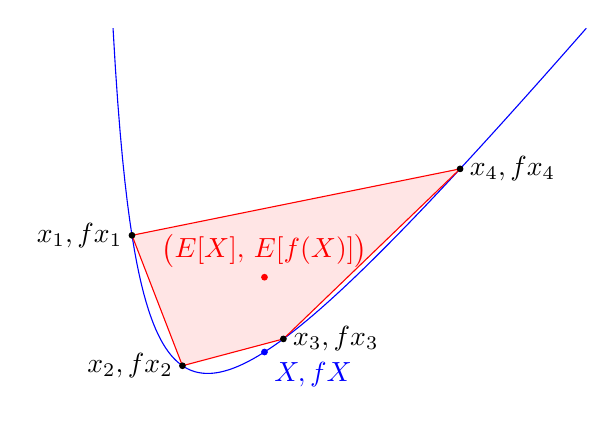
\begin{tikzpicture}
        \begin{axis}[
            axis lines = none,
            xmin = -2, xmax = 4.5,
            ymin = 0, ymax = 4.5,
            samples = 200,
            domain = 0.25:4,
            width = 12cm
        ]

        \addplot[no marks, blue]{1 / x + x};

        \pgfmathsetmacro{\xa}{0.4}
        \pgfmathsetmacro{\xb}{0.8}
        \pgfmathsetmacro{\xc}{1.6}
        \pgfmathsetmacro{\xd}{3}
        \pgfmathsetmacro{\xe}{(\xa + \xb + \xc + \xd) / 4}

        \pgfmathsetmacro{\fa}{1 / \xa + \xa}
        \pgfmathsetmacro{\fb}{1 / \xb + \xb}
        \pgfmathsetmacro{\fc}{1 / \xc + \xc}
        \pgfmathsetmacro{\fd}{1 / \xd + \xd}
        \pgfmathsetmacro{\fe}{1 / \xe + \xe}

        \pgfmathsetmacro{\ef}{(\fa + \fb + \fc + \fd) / 4}

        \addplot[only marks, mark=*, mark size=1pt]
                coordinates {(\xa, \fa) (\xb, \fb) (\xc, \fc) (\xd, \fd)};

        \node[left] at (axis cs:\xa, \fa) {\(\para{x_1, f\para{x_1}}\)};
        \node[left] at (axis cs:\xb, \fb) {\(\para{x_2, f\para{x_2}}\)};
        \node[right] at (axis cs:\xc, \fc) {\(\para{x_3, f\para{x_3}}\)};
        \node[right] at (axis cs:\xd, \fd) {\(\para{x_4, f\para{x_4}}\)};

        \addplot[
            fill=red!10,
            draw=red
        ]
        coordinates {
            (\xa, \fa)
            (\xb, \fb)
            (\xc, \fc)
            (\xd, \fd)
            (\xa, \fa)
        };

        \addplot[only marks, mark=*, mark size=1pt, blue]
            coordinates {(\xe,\fe)};
        \node[blue, below right] at (axis cs:\xe, \fe) {\(\para{\Expt\brac{X}, f\para{\Expt\brac{X}}}\)};

        % (E[X], E[f(X)]) point
        \addplot[only marks, mark=*, mark size=1pt, red]
            coordinates {(\xe,\ef)};

        \node[red, above] at (axis cs:\xe,\ef)
            {$\bigl(\mathbb E[X],\,\mathbb E[f(X)]\bigr)$};
        \end{axis}
    \end{tikzpicture}

    \caption{Jensen's Inequality}
    \label{fig:jensen-inequality}
\end{figure}

A trick to remembering the direction of the inequality is that since
\[
    \Var\para{X} = \Expt\brac{\para{X - \Expt\brac{X}}^2} \geq 0
\]
and also
\[
    \Var\para{X} = \Expt\brac{X^2} - \Expt\brac{X}^2,
\]
and note \(f\para{x} = x^2\) is convex and
\[
    \Expt\brac{X^2} \geq \para{\Expt\brac{X}}^2.
\]

To visualise \autoref{thm:jensen} (Jensen's Inequality), \autoref{fig:jensen-inequality} considers a uniform distribution over \(\brce{x_1, x_2, x_3, x_4}\), and the centre of the quadrilateral is marked red, with \(y\)-coordinate \(\Expt\brac{f\para{X}}\), while \(f\para{\Expt\brac{X}}\) is marked as the blue dot on the curve.

We first produce useful lemmas for the proof.

\begin{lemma}[Convex Function lies above Tangents]
    \label{lem:convex-fn-tangents}%
    A convex function \(\functiondomain{f}{\RR}{\RR}\) is the supremum of all the lines lying below it. In other words,
    \[
        \forall m \in \RR, \exists a, b \in \RR: f\para{m} = am + b \land \forall x \in \RR: f\para{x} \geq ax + b.
    \]
\end{lemma}

\begin{figure}[ht!]
    \centering
    \begin{tikzpicture}
        \begin{axis}[
            axis lines = middle,
            xlabel = {\(x\)},
            ylabel = {\(f(x)\)},
            xmin = -1, xmax = 5,
            ymin = -2, ymax = 9,
            xtick = \empty,
            ytick = \empty,
            domain = 0:4,
            samples = 100,
            width = 10cm
        ]

            \addplot[no marks, thick, blue] {0.5*x^2};

            \addplot[only marks, mark=*, mark size = 1pt] coordinates {(1, 0.5) (2, 2) (3, 4.5)};

            \addplot[domain=0.25:4.5] {1 * (x - 1) + 0.5};
            \addplot[domain=0.4:4.2] {2 * (x - 2) + 2};
            \addplot[domain=0.5:4.1] {3 * (x - 3) + 4.5};
        \end{axis}
    \end{tikzpicture}

    \caption{Convex Function and its Tangents}
    \label{fig:convex-fn-tangents}
\end{figure}

\autoref{fig:convex-fn-tangents} visualises this.

\begin{proof}
    Let \(m \in \RR\) and \(x < m < y\). Then
    \[
        m = tx + \para{1 - t}y
    \]
    for some \(t \in \oointv{0}{1}\). This gives
    \[
        t\para{m - x} = \para{1 - t} \para{y - m}.
    \]

    By convexity,
    \[
        f\para{m} = f\para{tx + \para{1 - t} y} \leq t f\para{x} + \para{1 - t} f\para{y}
    \]
    and hence
    \[
        t\para{f\para{m} - f\para{x}} \leq \para{1 - t} \para{f\para{y} - f\para{m}}.
    \]

    Hence,
    \[
        \frac{f\para{m} - f\para{x}}{m - x} \leq \frac{f\para{y} - f\para{m}}{y - m}.
    \]

    Let
    \[
        a = \sup_{x < m} \frac{f\para{m} - f\para{x}}{m - x}.
    \]

    Then, from the previous inequality on the gradients,
    \[
        \frac{f\para{m} - f\para{x}}{m - x} \leq a \leq \frac{f\para{y} - f\para{m}}{y - m}.
    \]

    So this gives that
    \[
        f\para{z} \geq a\para{z - m} + f\para{m},
    \]
    for all \(z \in \RR\), with the equal sign taking place if \(z = m\).
\end{proof}

Now we use \autoref{lem:convex-fn-tangents} to prove \autoref{thm:jensen} (Jensen's Inequality).

\begin{proof}[of \autoref{thm:jensen} (Jensen's Inequality)]
    Let \(m = \Expt\brac{X}\). By the claim, there is some \(a, b \in \RR\), such that
    \[
        f\para{m} = am + b
    \]
    and
    \[
        f\para{x} \geq ax + b
    \]
    for all \(x\). Then, we have
    \[
        f\para{X} \geq aX + b.
    \]

    Taking expectations on both sides, we get
    \[
        \Expt\brac{f\para{X}} \geq a \Expt\brac{X} + b = am + b = f\para{m} = f\para{\Expt\brac{X}}.
    \]
\end{proof}

Combining both \autoref{lem:convex-fn-tangents}, we can produce a proof as follows.

\begin{proof}[of \autoref{thm:jensen} (Jensen's Inequality), combining \autoref{lem:convex-fn-tangents}]
    Let \(m = \Expt\brac{X}\). For any \(x < m < y\), let \(t \in \ccintv{0}{1}\) be such that
    \[
        m = tx + \para{1 - t} y.
    \]

    Then,
    \[
        t \para{m - x} = \para{1 - t} \para{y - m}. \eqno{(\dagger)}
    \]

    By convexity condition,
    \[
        f \para{m} \leq t x + \para{1 - t} f\para{y},
    \]
    so
    \[
        t \para{f\para{m} - f\para{x}} \leq \para{1 - t} \para{f\para{y} - f\para{m}}. \eqno{(\ddagger)}
    \]

    Dividing \((\ddagger)\) by \((\dagger)\) (since it is positive), we have for all \(x < m < y\), that
    \[
        \frac{f\para{m} - f\para{x}}{m - x} \leq \frac{f\para{y} - f\para{m}}{y - m}.
    \]

    Define
    \[
        a = \sup_{x < m} \frac{f\para{m} - f\para{x}}{m - x},
    \]
    then we have for all \(x < m < y\), that
    \[
        \frac{f\para{m} - f\para{x}}{m - x} \leq a \leq \frac{f\para{y} - f\para{m}}{y - m},
    \]
    so for all \(z \in \RR\) (by dealing with cases \(z < x\) and \(z > y\) using the inequality above)
    \[
        f\para{z} \geq f\para{m} + a \para{x - m}.
    \]

    Therefore,
    \[
        f\para{X} \geq f\para{\Expt\brac{X}} + a \para{x - \Expt\brac{X}},
    \]  
    and taking expectations on both sides, we have
    \[
        \Expt\brac{f\para{X}} \geq f\para{\Expt\brac{X}} + a \para{\Expt\brac{X} - \Expt\brac{X}} = f\para{\Expt\brac{X}}
    \]
    as desired.
\end{proof}

Similar to when we study Cauchy--Schwartz back then, we study the cases of equality.

Let \(\functiondomain{f}{\RR}{\RR}\) be convex, and with the extra property that for \(m = \Expt\brac{X}\), there is some \(a, b \in \RR\), such that
\[
    f\para{m} = am + b \land \forall x \in \RR \setminus \brce{m}: f\para{x} > ax + b,
\]
i.e. let \(f\) be strictly convex at \(m\). Note that 
\[
    f\para{X} - \para{aX + b} \geq 0.
\]

Taking expectation on both sides, we have
\[
    \Expt\brac{f\para{X}} \geq a \Expt\brac{X} + b = am + b = f\para{m} = f\para{\Expt\brac{X}}.
\]

We want that \(\Expt\brac{f\para{X}} = f\para{\Expt\brac{X}}\), so this forces
\[
    \Expt\brac{f\para{X} - \para{aX + b}} = 0
\]
which implies that
\[
    \Prob\para{f\para{X} = aX + b} = 1.
\]

But this now forces \(X = m\), so \(\Prob\para{X = m} = 1\).

There is a nice result due to Jensen's Inequality.

\begin{theorem}[AM--GM Inequality]
    \label{thm:am-gm}
    Let \(f\) be a convex function. Then we have for all \(x_1, \ldots, x_n \in \RR\), we have
    \[
        \frac{1}{n} \sum_{k = 1}^{n} f\para{x_k} \geq f\para{\frac{\sum_{k = 1}^{n} x_k}{n}}.
    \]
\end{theorem}

\begin{proof}
    We take \(X\) to be a random variable, with \(X \sim \Uniform \brce{x_1, x_2, \ldots, x_n}\), with \(\Prob\para{X = x_i} = \frac{1}{n}\) for \(i = 1, 2, \ldots, n\).

    Hence,
    \[
        \frac{1}{n} \sum_{k = 1}^{n} f\para{x_k} = \Expt\brac{f\para{X}} = \sum_{x \in \RR} f\para{x} \Prob\para{X = x}.
    \]

    By \autoref{thm:jensen} (Jensen's Inequality), we have
    \[
        \Expt\brac{f\para{X}} \geq f\para{\Expt\brac{X}} = f\para{\frac{\sum_{k = 1}^{n} x_k}{n}}.
    \]
\end{proof}

\begin{remark}
    The more commonly seen AM--GM inequality is a corollary of this. Let \(f\para{x} = - \log x\), for \(x > 0\). Take \(x_1, \ldots, x_n > 0\), we have
    \[
        - \frac{1}{n} \sum_{k = 1}^{n} \log x_k \geq - \log \para{\frac{\sum_{k = 1}^{n} x_k}{n}}.
    \]

    Exponentiating both sides, we get
    \[
        \para{\prod_{k = 1}^{n} x_k}^{\frac{1}{n}} \leq \frac{1}{n} \sum_{k = 1}^{n} x_k.
    \]
\end{remark}
\section{Joint Distribution}

Recall that, if \(X\) is a discrete random variable then the distribution of \(X\) is \(\para{\Prob\para{X = x}}_x\).

\subsection{Joint Distribution}

\begin{definition}[Joint Distribution for Discrete Variables]
    \label{def:joint-distribution-discrete}%
    Let \(X_1, \ldots, X_n\) be discrete random variables. Their \emph{joint distribution} is defined to be
    \[
        \Prob\para{X_1 = x_1, \ldots, X_n = x_n}
    \]
    for all possible values of \(x_1, x_2, \ldots, x_n\).
\end{definition}

Note that we could recover the individual distribution of a single random variable from this as well. Indeed, we have
\[
    \Prob\para{X_1 = x_1} = \sum_{x_2, \ldots, x_n \in \RR} \Prob\para{X_1 = x_1, \ldots, X_n = x_n}
\]
where we note that this sum is countable since \(x_i\)s only take countably many values. We call this the \emph{marginal distribution} of \(X_1\).

\begin{definition}[Conditional Distribution for Discrete Variables]
    \label{def:conditional-distribution-discrete}%
    Let \(X\) and \(Y\) be two discrete random variables. The \emph{conditional distribution} of \(X\), given \(Y = y\) (where \(y\) is fixed) is defined to be
    \[
        \Prob\para{\Conditional{X = x}{Y = y}} = \frac{\Prob\para{X = x, Y = y}}{\Prob\para{Y = y}}
    \]
    for all possible values of \(x\).
\end{definition}

By \autoref{thm:law-total-probability} (Law of Total Probability), we have
\[
    \Prob\para{X = x} = \sum_{y \in \RR} \Prob\para{\Conditional{X = x}{Y = y}} \cdot \Prob\para{Y = y}
\]
noting that this sum is similarly countable.

\subsection{Sum of Random Variables}

\begin{example}[Distribution of Sum of Random Variables]
    \label{ex:distribution-sum-discrete}%
    Let \(X\) and \(Y\) be two independent random variables. We = want to understand the distribution of \(X + Y\). We have
    \begin{align*}
        \Prob\para{X + Y = z} &= \sum_{y \in \RR} \Prob\para{X + Y = z, Y = y} \\
        &= \sum_{y \in \RR} \Prob\para{X = z - y, Y = y} \\
        &= \sum_{y \in \RR} \Prob\para{X = z - y} \cdot \Prob\para{Y = y}.
    \end{align*}
\end{example}

\begin{definition}[Convolution of Distribution for Discrete Variables]
    \label{def:convolution-distribution-discrete}%
    Let \(X, Y\) be two discrete random variables. Then the distribution of \(X + Y\), given by
    \[
        \sum_{y \in \RR} \Prob\para{X = z - y} \cdot \Prob\para{Y = y}
    \]
    is known as the \emph{convolution} of the two random variables.
\end{definition}

\begin{example}[Sum of Poisson Random Variables]
    Let \(X \sim \Poisson\para{\lambda}\), \(Y \sim \Poisson\para{\mu}\), \(\lambda, \mu > 0\) and \(X \indp Y\). We may show that the sum of two independent Poisson random variables is another Poisson random variable.

    \begin{align*}
        \Prob\para{X + Y = n} &= \sum_{k = 0}^{n} \Prob\para{X = n - k} \cdot \Prob\para{Y = k} \\
        &= \sum_{k = 0}^{m} e^{-\lambda} \cdot \frac{\lambda^{n - k}}{\para{n - k}!} \cdot e^{-\mu} \cdot \frac{\mu^k}{k!} \\
        &= e^{-\para{\lambda + \mu}}{n!} \cdot \sum_{k = 0}^{n} \binom{n}{k} \cdot \lambda^{n - k} \cdot \mu^k \\
        &= e^{-\para{\lambda + \mu}} \cdot \frac{\para{\lambda + \mu}^n}{n!}.
    \end{align*}

    Therefore, we have
    \[
        \Prob\para{X + Y = n} = e^{-\para{\lambda + \mu}} \cdot \frac{\para{\lambda + \mu}^n}{n!}
    \]
    and hence
    \[
        X + Y \sim \Poisson \para{\lambda + \mu}.
    \]

    Indeed, if \(\lambda = \mu\), let \(X_n, Y_n \sim \Binomial\para{n, \frac{\lambda}{n}}\) and \(X_n \indp Y_n\). We know a Poisson distribution is a limit of binomial random variables, and indeed
    \[
        X_n + Y_n \sim \Binomial\para{2n, \frac{\lambda}{n}}.
    \]
\end{example}

\subsection{Conditional Expectation}

\begin{definition}[Conditonal Expectation upon an Event]
    \label{def:conditional-expectation-upon-event}%
    The \emph{conditional expectation} of a random variable \(X\) with respect to an event \(B\), where \(\Prob\para{B} > 0\), is given by
    \[
        \Expt\brac{\Conditional{X}{B}} = \frac{\Expt\brac{X \cdot \indicator\para{B}}}{\Prob\para{B}}.
    \]
\end{definition}

Note that with \(X = \indicator\para{A}\), we do recover consistent definitions with conditional probability of events.

\[
    \Expt\brac{\Conditional{\indicator\para{A}}{B}} = \frac{\Expt\brac{\indicator\para{A} \cdot \indicator\para{B}}}{\Prob\para{B}} = \frac{\Expt\brac{\indicator\para{A \cap B}}}{\Prob\para{B}} = \frac{\Prob\para{A \cap B}}{\Prob\para{B}} = \Prob\para{\Conditional{A}{B}}.
\]

\begin{theorem}[Law of Total Expectation]
    \label{thm:law-of-total-expectation}%
    Let \(X\) be a random variable, \(\para{\Omega_i}\) be a partition of \(\Omega\) into disjoint sets, with \(\Prob\para{\Omega_i} > 0\) for all \(i = 1, 2, \ldots ,n\). Then we have
    \[
        \Expt\brac{X} = \sum_{i = 1}^{n} \Expt\brac{\Conditional{X}{\Omega_n}} \cdot \Prob\para{\Omega_n}.
    \]
\end{theorem}

\begin{proof}
    We have
    \begin{align*}
        \Expt\brac{X} &= \Expt\brac{X \cdot \indicator\para{\Omega}} \\
        &= \Expt\brac{X \cdot \sum_{i = 1}^{n} \indicator \para{\Omega_i}} \\
        &= \sum_{i = 1}^{n} \Expt\brac{X \cdot \indicator \para{\Omega_i}} \\
        &= \sum_{i = 1}^{N} \Expt\brac{\Conditional{X}{\Omega_n}} \cdot \Prob\para{\Omega_n}
    \end{align*}
\end{proof}

The conditional expectation of \(X\) given \(Y = y\) is defined similarly, since \(Y = y\) is an event:
\[
    \Expt\brac{\Conditional{X}{Y = y}} = \frac{\Expt\brac{X \cdot \indicator\para{Y = y}}}{\Prob\para{Y = y}}.
\]

\begin{proposition}[Conditional Expectation upon Random Variable Event]
    \label{prop:conditional-expectation-random-variable}%
    We have
    \[
        \Expt\brac{\Conditional{X}{Y = y}} = \sum_{x \in \RR} x \cdot \Prob\para{\Conditional{X = x}{Y = y}}.
    \]
\end{proposition}

\begin{proof}
    We have
    \begin{align*}
        \Expt\brac{\Conditional{X}{Y = y}} &= \frac{\Expt\brac{X \cdot \indicator\para{Y = y}}}{\Prob\para{Y = y}} \\
        &= \sum_{x \in \RR} x \cdot \frac{\Prob\para{X = x, Y = y}}{\Prob\para{Y = y}} \\
        &= \sum_{x \in \RR} x \cdot \Prob\para{\Conditional{X = x}{Y = y}}.
    \end{align*}
\end{proof}

This shows that the conditional expectation is consistent with the expectation of the conditional random variable.

\begin{definition}[Conditional Expectation Distribution]
    \label{def:conditional-expectation-distribution}%
    We define \(\Expt\brac{\Conditional{X}{Y}}\) as a random variable as
    \[
        \Expt\brac{\Conditional{X}{Y}} = g\para{Y} = \sum_{y \in \RR} g\para{y} \cdot \indicator\para{Y = y},
    \]
    where
    \[
        g\para{y} = \Expt\brac{\Conditional{X}{Y = y}}.
    \]
\end{definition}

This notation may seem confusing at the start. For example, if \(g\para{y} = y^2\), we have
\[
    \Expt\brac{\Conditional{X}{Y}} = g\para{Y} = Y^2.
\]

Intuitively, this is the \textbf{best approximation} of \(X\) using the random variable \(Y\). In the two extreme cases, if \(X = f\para{Y}\), then we have
\[
    \Expt\brac{\Conditional{X}{Y}} = f\para{Y},
\]
and if \(X \indp Y\), we have
\[
    \Expt\brac{\Conditional{X}{Y}} = \Expt\brac{X}.
\]

As a function, we may define it for \(\omega \in \Omega\),
\[
    \Expt\brac{\Conditional{X}{Y}}\para{\omega} = \Expt\brac{\Conditional{X}{Y = Y\para{\omega}}}.
\]

\begin{example}[Conditional Expectation for Tossing \(p\)-Coin]
    \label{ex:conditional-expectatio-tossing-p-coin}%
    Toss a \(p\)-coin independently for \(n\) times. Let \(X_i\) be the indicator that the \(i\)th toss is a head, for \(i = 1, 2, \ldots, n\), and let \(Y_n = X_1 + X_2 + \cdots + X_n\).

    We set \(g\para{y} = \Expt\brac{\Conditional{X_1}{Y_n = y}}\). Note that
    \begin{align*}
        g\para{y} &= \Expt\brac{\Conditional{X_1}{Y_n = y}} \\
        &= \frac{\Expt\brac{X_1 \cdot \indicator\para{Y_n = y}}}{\Prob\para{Y_n = y}} \\
        &= \frac{\Prob\para{X_1 = 1, Y_n = y}}{\Prob\para{Y_n = y}} \\
        &= \frac{p \cdot \binom{n - 1}{y - 1} \cdot p^{y - 1} \cdot \para{1 - p}^{n - y}}{\binom{n}{y} \cdot p^y \cdot \para{1 - p}^{n - y}} \\
        &= \frac{y}{n}.
    \end{align*}

    Hence,
    \[
        \Expt\brac{\Conditional{X_1}{Y_n}} = \frac{Y_n}{n}.
    \]

    Indeed, this makes sense, since one would probably expect each \(X_i\) to be \(\frac{Y}{n}\) `on average'.
\end{example}

\begin{proposition}[Properties of Conditional Expectation Distribution]
    \label{prop:conditional-expectation-distribution-property}%
    For any \(c \in \RR\), we have
    \begin{itemize}
        \item \(\Expt\brac{\Conditional{cX}{Y}} = c \Expt\brac{\Conditional{X}{Y}}\).
        \item \(\Expt\brac{\Conditional{c + X}{Y}} = c + \Expt\brac{\Conditional{X}{Y}}\) and \(\Expt\brac{\Conditional{c}{Y}} = c\).
        \item If \(X_1, X_2, \ldots, X_n\) and \(Y\) are random variables, then we have
        \[
            \Expt\brac{\Conditional{\sum_{i = 1}^{n} X_i}{Y}} = \sum_{i = 1}^{n} \Expt\brac{\Conditional{X_i}{Y}}.
        \]
    \end{itemize}
\end{proposition}

\begin{proposition}[Expectation of Conditional Expectation Distribution]
    \label{prop:expectation-conditional-expectation-distribution}%
    We have
    \[
        \Expt\brac{\Expt\brac{\Conditional{X}{Y}}} = \Expt\brac{X}.
    \]
\end{proposition}

\begin{proof}
    Recall that
    \[
        \Expt\brac{\Conditional{X}{Y}} = \sum_{y \in \RR} \indicator\para{Y = y} \Expt\brac{\Conditional{X}{Y = y}}.
    \]

    Taking the expectations on both sides, we have
    \[
        \Expt\brac{\Expt\brac{\Conditional{X}{Y}}} = \sum_{y \in \RR} \Prob\para{Y = y} \cdot \Expt\brac{\Conditional{X}{Y = y}} = \Expt\brac{X}.
    \]
\end{proof}

\begin{proposition}[Conditional Expectation Distribution of Independent Variables]
    \label{prop:conditional-expectation-distribution-independent}%
    Let \(X\) and \(Y\) be independent. Then
    \[
        \Expt\brac{\Conditional{X}{Y}} = \Expt\brac{X}.
    \]
\end{proposition}

\begin{proof}
    Recall that by definition,
    \begin{align*}
        \Expt\brac{\Conditional{X}{Y = y}} &= \sum_{x \in \RR} x \cdot \Prob\para{\Conditional{X = x}{Y = y}} \\
        &= \sum_{x \in \RR} x \cdot \Prob\para{X = x} \\
        &= \Expt\brac{X}.
    \end{align*}

    Hence,
    \[
        \Expt\brac{\Conditional{X}{Y}} = \Expt\brac{X} \sum_{y \in \RR} \indicator\para{Y = y} = \Expt\brac{X}
    \]
    as desired.
\end{proof}

\begin{proposition}[Conditional Expectation upon Independent Conditions]
    \label{prop:conditional-expectation-independent-conditions}%
    Let \(Y\) and \(Z\) be two independent random variables. Then
    \[
        \Expt\brac{\Conditional{\Expt\brac{\Conditional{X}{Y}}}{Z}} = \Expt\brac{X}.
    \]
\end{proposition}

\begin{proof}
    Set \(g\para{Y} = \Expt\brac{\Conditional{X}{Y}}\), while \(g\para{y} = \Expt\brac{\Conditional{X}{Y = y}}\).

    First, we claim that \(g\para{Y}\) is independent of \(Z\). We want to show that for all \(w, z\), we have
    \[
        \Prob\para{g\para{Y} = w, Z = z} = \Prob\para{g\para{Y} = w} \cdot \Prob\para{Z = z}.
    \]

    We have
    \begin{align*}
        \Prob\para{g\para{Y} = w, Z = z} &= \sum_{y \in g\inverse\para{\brce{w}}} \Prob\para{Y = y, Z = z} \\
        &= \sum_{y \in g\inverse\para{\brce{w}}} \Prob\para{Y = y} \cdot \Prob\para{Z = z} \\
        &= \Prob\para{Z = z} \cdot \sum_{y \in g\inverse\para{\brce{w}}} \Prob\para{Y = y} \\
        &= \Prob\para{Z = z} \cdot \Prob\para{g\para{Y} = w}.
    \end{align*}

    Therefore, \(g\para{Y} \indp Z\).

    Therefore, by \autoref{prop:conditional-expectation-distribution-independent} we have
    \[
        \Expt\brac{\Conditional{\Expt\brac{\Conditional{X}{Y}}}{Z}} = \Expt\brac{\Conditional{g\para{Y}}{Z}} = \Expt\brac{g\para{Y}},
    \]
    and we have from \autoref{prop:expectation-conditional-expectation-distribution},
    \[
        \Expt\brac{g\para{Y}} = \Expt\brac{\Expt\brac{\Conditional{X}{Y}}} = \Expt\brac{X}.
    \]
\end{proof}

\begin{proposition}[Extraction of Function of Condition]
    \label{prop:extraction-function-condition}%
    For any function \(\functiondomain{h}{\RR}{\RR}\), we have
    \[
        \Expt\brac{\Conditional{h\para{Y} \cdot X}{Y}} = h\para{Y} \cdot \Expt\brac{\Conditional{X}{Y}}.
    \]
\end{proposition}

\begin{proof}
    We have
    \begin{align*}
        \Expt\brac{\Conditional{h\para{Y} \cdot X}{Y}} &= \sum_{y \in \RR} \indicator\para{Y = y} \cdot \Expt\brac{\Conditional{h\para{Y} \cdot X}{Y = y}} \\
        &= \sum_{y \in \RR} \indicator\para{Y = y} \cdot h\para{Y} \cdot \Expt\brac{\Conditional{X}{Y = y}} \\
        &= h\para{Y} \cdot \sum_{y \in \RR} \indicator\para{Y = y} \cdot \Expt\brac{\Conditional{X}{Y = y}} \\
        &= h\para{Y} \cdot \Expt\brac{\Conditional{X}{Y}}.
    \end{align*}
\end{proof}

We have two corollaries due to the properties above.

\begin{corollary}[Conditional Expectation upon Same Condition]
    \label{cor:conditional-expecation-upon-same-condition}%
    We have
    \[
        \Expt\brac{\Conditional{\Expt\brac{\Conditional{X}{Y}}}{Y}} = \Expt\brac{\Conditional{X}{Y}}.
    \]
\end{corollary}

\begin{corollary}[Conditional Expectation upon Itself]
    \label{cor:conditional-expectation-upon-itself}%
    We have
    \[
        \Expt\brac{\Conditional{X}{X}} = X.
    \]    
\end{corollary}

\begin{example}[Conditional Expectation for Tossing \(p\)-Coin, Revisited]
    \label{ex:conditional-expectatio-tossing-p-coin-revisited}%
    We revisit \autoref{ex:conditional-expectatio-tossing-p-coin}. We toss a \(p\)-coin \(n\) times independently. Let \(X_i = \indicator\para{i\text{-th toss is H}}\) for \(i = 1, 2, \ldots, n\), and let
    \[
        Y_n = X_1 + \cdots + X_n.
    \]

    By symmetry, for all \(i = 1, 2, \ldots, n\), we have
    \[
        \Expt\brac{\Conditional{X_i}{Y_n}} = \Expt\brac{\Conditional{X_1}{Y_n}}
    \]

    Note that
    \[
        \Expt\brac{\Conditional{\sum_{i = 1}^{n} X_i}{Y_n}} = \Expt\brac{\Conditional{Y_n}{Y_n}} = Y_n,
    \]
    while using linearity gives
    \[
        \Expt\brac{\Conditional{\sum_{i = 1}^{n} X_i}{Y_n}} = \sum_{i = 1}^{n} \Expt\brac{\Conditional{X_i}{Y_n}} = n \cdot \Expt\brac{\Conditional{X_1}{Y_n}}.
    \]

    Hence,
    \[
        \Expt\brac{\Conditional{X_1}{Y_n}} = \frac{Y_n}{n}.
    \]
\end{example}
\section{Random Walk}

\begin{definition}[Random/Stochastic Process]
    \label{def:random-stochastic-process}%
    A \emph{random/stochastic process} is a sequence of random variables \(\para{X_n}_{n \in \NN}\).
\end{definition}

\begin{definition}[Random Walk]
    \label{def:random-walk}%
    A \emph{random walk} is a random process that can be expressed in the following way:
    \[
        X_n = x + \sum_{i = 1}^{n} Y_i,
    \]
    where \(x\) is a deterministic number, and \(\para{Y_i}_{n \in \NN}\)s are independent and identically distributed (i.i.d.). The random variables \(Y_i\)s the \emph{steps} of the random walk.
\end{definition}

\begin{definition}[Simple Random Walk]
    \label{def:simple-random-walk}%
    A random walk is \emph{simple} if the steps can only take values \(\pm 1\).
\end{definition}

In this case, we may set \(\Prob\para{Y_i = 1} = p\) and \(\Prob\para{Y_i = -1} = q\), with \(p + q = 1\) and \(p, q \geq 0\).

\begin{notation}
    We denote \(\Prob_x\para{A} = \Prob\para{\Conditional{A}{X_0 = x}}\) and \(\Expt_x\brac{A} = \Expt\brac{\Conditional{A}{X_0 = x}}\).
\end{notation}

\begin{example}[Gambler's Ruin Estimates]
    \label{ex:gambler-ruin-estimates}%
    We may think of \(\para{X_n}\) as the fortune of a gambler, who starts with \(x\) in their pocket at time \(0\), and every time step they bet \(1\), which he loses with probability \(\para{1 - p}\), and gets it back doubled with probability \(p\). The game ends if they reach \(0\) (which means they go bankrupt) or they reach \(a\), whichever happens first.

    We want to know the probability they reach \(a\) before going bankrupt. We let
    \[
        h\para{x} = \Prob_x \para{\para{X_n} \text{ reaches }a\text{ before reaching }0}.
    \]

    Note that \(h\para{0} = 0\) and \(h\para{a} = 1\). We have
    \begin{align*}
        h\para{x} &= \Prob_x \para{X \text{ reaches }a\text{ before }0} \\
        &= \Prob_x \para{\Conditional{X \text{ reaches }a\text{ before }0}{Y_1 = 1}} \cdot p + \Prob_x \para{\Conditional{X \text{ reaches }a\text{ before }0}{Y_1 = -1}} \cdot \para{1 - p} \\
        &= p \cdot h \para{x + 1} + \para{1 - p} \cdot h \para{x - 1}.
    \end{align*}

    We now consider particular cases of \(p\) and \(q\).

    \begin{itemize}
        \item If \(p = q = \frac{1}{2}\), this is called \emph{simple symmetric random walk}, and the system reduces to \(h\para{x} = \frac{1}{2} h \para{x + 1} + \frac{1}{2} h \para{x - 1}\).
        
        Notice that simplifying this gives
        \[
            h\para{x + 1} - h\para{x} = h\para{x} - h\para{x - 1} = \cdots = c.
        \]

        Therefore, we have \(h\para{x} = \sum_{i = 1}^{x} \para{h\para{i} - h\para{i - 1}} = cx\). Since \(h\para{a} = 1\), we have \(c = \frac{1}{a}\), so \(h\para{x} = \frac{x}{a}\).

        \item If \(p \neq q\), we first try a solution of the form \(\lambda^x\) for some \(\lambda\). We have
        \[
            \lambda^x = p \cdot \lambda^{x + 1} + q \cdot \lambda^{x - 1}
        \]
        and hence \(\lambda = 1\) or \(\lambda = \frac{q}{p}\). Therefore, the general solution gives
        \[
            h\para{x} = A + B \cdot \para{\frac{q}{p}}^x.
        \]

        Putting in the boundary conditions, we have
        \[
            h\para{x} = \frac{\para{\frac{q}{p}}^x - 1}{\para{\frac{q}{p}}^a - 1}.
        \]
    \end{itemize}
\end{example}

\begin{example}[Time to Absorption]
    \label{ex:time-to-absorption}%
    We use a similar setup as \autoref{ex:gambler-ruin-estimates}. Let the \emph{time to absorption} be
    \[
        T = \min \set{n \geq 0}{X_n \in \brce{0, a}}.
    \]

    \(T\) is the first \(n\) such that \(X_n\) is either \(0\) or \(a\). In other words, \(T\) is the duration of the game.

    We aim to find \(\Expt\brac{\Conditional{T}{X_0 = x}} = \Expt_x\brac{T}\). Let this be \(k\para{x}\).

    Using the law of total expectation, we have
    \begin{align*}
        k\para{x} &= \Expt_x\brac{\Conditional{T}{Y_1 = 1}} \cdot \Prob\para{Y_1 = 1} + \Expt_x\brac{\Conditional{T}{Y_1 = -1}} \cdot \Prob\para{Y_1 = -1} \\
        &= p \cdot \para{1 + k\para{x + 1}} + \para{1 - p} \cdot \para{1 + k\para{x - 1}} \\
        &= 1 + p \cdot k\para{x + 1} + q \cdot k\para{x - 1}.
    \end{align*}

    The initial conditions are \(k \para{0} = k \para{a} = 0\).
    \begin{itemize}
        \item If \(p = q = \frac{1}{2}\), we experiment with a solution of the form \(A x^2\). We have
        \[
            A x^2 = 1 + p A\para{x + 1}^2 + q A\para{x - 1}^2.
        \]

        Hence, \(A = -1\), and the general solution is
        \[
            k\para{x}= -x^2 + Bx + C.
        \]

        With the initial conditions, we have
        \[
            k\para{x} = x \para{a - x}.
        \]

        \item If \(p \neq q\), we experiment with a solution of the form \(Cx\). We have
        \[
            C = \frac{1}{q - p}
        \]
        giving general solution
        \[
            k\para{x} = A + \frac{1}{q - p} \cdot x + B \cdot \para{\frac{q}{p}}^x,
        \]

        Hence, putting in the initial conditions, we have
        \[
            k\para{x} = \frac{1}{q - p} \cdot x - \frac{a}{q - p} \cdot \frac{\para{\frac{q}{p}}^x - 1}{\para{\frac{q}{p}}^a - 1}.
        \]
    \end{itemize}
\end{example}
\section{Probability Generating Functions}

Note that all natural numbers \(\NN\) in this section includes \(0\).

Let \(X\) be a random variable with values in \(\NN\). We denote the probability mass function of \(X\) as
\[
    p_r = \Prob\pqty{X = r}, \quad r \in \NN.
\]

\subsection{Definitions and Properties}

\begin{definition}[Probability Generating Function]
    \label{def:probability-generating-function}%
    The \emph{probability generating function} of \(X\) is defined to be
    \[
        p \pqty{z} = \Expt\bqty{z^X} = \sum_{r = 0}^{\infty} p_r \cdot z^r = p_0 + p_1 \cdot z + p_2 \cdot z^2 + \cdots
    \]
    where \(\abs{z} < 1\).
\end{definition}

Note that this infinite series is indeed well-defined. Taking the absolute value, we have
\begin{align*}
    \abs{p\pqty{z}} &= \abs{\sum_{r = 0}^{\infty} p_r \cdot z^r} \\
    &\leq \sum_{r = 0}^{\infty} p_r \cdot \abs{z^r} \\
    &\leq \sum_{r = 0}^{\infty} p_r \\
    &= 1,
\end{align*}
so the series converges absolutely for \(\abs{z} \leq 1\), and hence in particular, the radius of the convergence is at least \(1\).

\begin{theorem}[Uniqueness of Probability Generating Function]
    \label{thm:pgf-uniqueness}%
    The probability generating function uniquely determines the distribution of the random variable \(X\).
\end{theorem}

\begin{proof}
    Let \(\pqty{p_r}\) and \(\pqty{q_r}\) be two probability distributions with the same probability generating functions, i.e., for all \(\abs{z} \leq 1\), we have
    \[
        \sum_{r = 0}^{\infty} p_r z^r = \sum_{r = 0}^{\infty} q_r z^r.
    \]

    We want to show \(p_r = q_r\) for all \(r\). If we put in \(z = 0\), then we have \(p_0 = q_0\).

    We continue by strong induction. Suppose that \(p_r = q_r\) for all \(r \leq n\). We want to show that \(p_{n + 1} = q_{n + 1}\). By the induction hypothesis, we have
    \[
        \sum_{r = n + 1}^{\infty} p_r z^r = \sum_{r = n + 1}^{\infty} q_r z^r.
    \]

    Dividing by \(z^{n + 1}\), and set \(z = 0\), we have
    \[
        p_{n + 1} = q_{n + 1}.
    \]
\end{proof}

\begin{proposition}[Probability Generating Function of Sum]
    \label{prop:pgf-sum}%
    Let \(X_1, \ldots, X_n\) be independent random variables, with probability generating functions
    \[
        q_i\pqty{z} = \Expt\bqty{z^{X_i}}.
    \]

    Then, we have
    \[
        p\pqty{z} = q_1\pqty{z} \cdots q_n\pqty{z}.
    \]
\end{proposition}

\begin{proof}
    We have
    \begin{align*}
        p\pqty{z} &= \Expt\bqty{z^{X_1 + \cdots + X_n}} \\
        &= \Expt\bqty{z^{X_1}} \cdots \Expt\bqty{z^{x_n}}
    \end{align*}
    by independence, as desired.
\end{proof}

\subsection{Probability Generating Functions of Standard Distributions}

\begin{example}[Probability Generating Function of Binomial Distribution]
    \label{ex:pgf-binomial}%
    Suppose \(X \sim \Binomial\pqty{n, p}\). We have
    \begin{align*}
        p\pqty{z} = \Expt\bqty{z^X} &= \sum_{k = 0}^{n} z^k \cdot \binom{n}{k} \cdot p^k \cdot \pqty{1 - p}^{n - k} \\
        &= \pqty{pz + 1 - p}^n.
    \end{align*}
\end{example}

\begin{example}[Sum of Independent Binomial Distributions]
    \label{ex:sum-binomial}%
    Suppose \(X \sim \Binomial\pqty{n, p}\) and \(Y \sim \Binomial\pqty{m, p}\), with \(X \indp Y\). We want to find the distribution of \(\pqty{X + Y}\). We have
    \begin{align*}
        \Expt\bqty{z^{X + Y}} &= \Expt\bqty{z^X} \cdot \Expt\bqty{z^Y} \\
        &= \pqty{pz + 1 - p}^{n} \cdot \pqty{pz + 1 - p}^{m} \\
        &= \pqty{pz + 1 - p}^{n + m}.
    \end{align*}

    Therefore, \(X + Y \sim \Binomial\pqty{n + m, p}\).
\end{example}

\begin{example}[Probability Generating Function of Geometric Distribution]
    \label{ex:pgf-geometric}%
    Suppose \(X \sim \Geometric\pqty{p}\), where we use the convention of failures, starting from zero. Then
    \[
        \Expt\bqty{z^X} = \sum_{r = 0}^{\infty} z^r \pqty{1 - p}^r p = \frac{p}{1 - z\pqty{1 - p}}.
    \]
\end{example}

\begin{example}[Probability Generating Function of Poisson Distribution]
    \label{ex:pgf-poisson}%
    Suppose \(X \sim \Poisson\pqty{\lambda}\). Then
    \[
        \Expt\bqty{z^X} = \sum_{r = 0}^{\infty} z^r \cdot e^{-\lambda} \cdot \frac{\lambda^r}{r!} = e^{-\lambda} \cdot e^{\lambda z} = e^{\lambda \pqty{z - 1}}.
    \]
\end{example}

\begin{example}[Sum of Independent Poisson Distributions]
    Suppose \(X \sim \Poisson\pqty{\lambda}\), \(Y \sim \Poisson\pqty{\mu}\), and \(X \indp Y\). Then we have
    \[
        \Expt\bqty{z^{X + Y}} = e^{\lambda \pqty{z - 1}} \cdot e^{\mu\pqty{z - 1}} = e^{\pqty{\lambda + \mu} \pqty{z - 1}},
    \]
    so \(X + Y \sim \Poisson\pqty{\lambda + \mu}\).
\end{example}

\subsection{Expectation and Moments}

We now investigate how to find the expectation (and moments) using the probability generating function.

\begin{theorem}[Expectation from Probability Generating Function]
    \label{thm:expt-pgf}%
    We have
    \[
        \lim_{z \to 1^{-}} p'\pqty{z} = p'\pqty{1^{-}} = \Expt\bqty{X}.
    \]
\end{theorem}

\begin{proof}
    Suppose \(\Expt\bqty{X} < \infty\). Take \(0 < z < 1\), so
    \[
        p'\pqty{z} = \sum_{r = 1}^{\infty} r p_r z^{r - 1} \leq \sum_{r = 1}^{\infty} r p_r = \Expt\bqty{X}.
    \]

    Therefore, \(p'\pqty{z}\) is an increasing function of \(z\), and hence,
    \[
        \lim_{z \to 1^{-}} p'\pqty{z} \leq \Expt\bqty{X}.
    \]

    Let \(\epsilon > 0\). There exists \(N\) large, such that
    \[
        \sum_{r = 1}^{N} r p_r \geq \Expt\bqty{X} - \epsilon.
    \]

    Therefore,
    \[
        \lim_{z \to 1^{-}} p'\pqty{z} \geq \lim_{z \to 1^{-}} \sum_{r = 1}^{N} r p_r z^{r - 1} = \sum_{r = 1}^{N} r p_r \geq \Expt\bqty{X} - \epsilon.
    \]

    This finishes the proof.

    Now, suppose \(\Expt\bqty{X} = \infty\). Then for any \(M > 0\), there is some \(N \in \NN\), such that
    \[
        \sum_{r = 1}^{N} r p_r \geq M.
    \]

    Therefore, from before, we have
    \[
        \lim_{z \to 1^{-}} p'\pqty{z} \geq \lim_{z \to 1^{-}} \sum_{r = 1}^{N} r p_r z^{r - 1} = \sum_{r = 1}^{N} r p_r \geq M.
    \]

    Therefore, \(\lim_{z \to 1^{-}} p'\pqty{z} = \infty\).
\end{proof}

Similarly, we may find the factorial moments by taking the derivatives.

\begin{theorem}[Factorial Moments from Probability Generating Function]
    \label{thm:factorial-moments-pgf}%
    For the second factorial moment, we have
    \[
        p''\pqty{1^-} = \lim_{z \to 1^-} p''\pqty{z} = \Expt\bqty{X \pqty{X - 1}}.
    \]

    In general, for any \(k \geq 0\), we have
    \[
        p^{\pqty{k}} \pqty{1^-} = \lim_{z \to 1^-} p^{\pqty{k}}\pqty{z} = \Expt\bqty{X \pqty{X - 1} \cdots \pqty{X - k + 1}}.
    \]
\end{theorem}

\begin{corollary}[Variance from Probability Generating Function]
    \label{cor:var-pgf}%
    We have
    \[
        \Var\pqty{X} = p''\pqty{1^-} + p'\pqty{1^-} - \pqty{p'\pqty{1^-}}^2.
    \]
\end{corollary}

\begin{proposition}[Probability from Probability Generating Function]
    \label{prop:prob-pgf}%
    We have
    \[
        \Prob\pqty{X = n} = p^{\pqty{n}} \pqty{0} \cdot \frac{1}{n!}.
    \]
\end{proposition}

\subsection{Sum of a Random Number of Random Variables}

Let \(X_1, X_2, \ldots\) be independent and identically distributed, and let \(N\) be a random variable (independent) and take values in \(\NN\).

We set the sum
\[
    S_n = X_1 + \cdots + X_n = \sum_{i = 1}^{n} X_i,
\]
and as a function,
\[
    S_n\pqty{\omega} = \sum_{i = 1}^{n} X_i\pqty{\omega}.
\]

\begin{definition}[Sum of a Random Number of Random Variables]
    \label{def:sum-random-number-rvs}%
    We define
    \[
        S_N \pqty{\omega} = S_{N\pqty{\omega}} \pqty{\omega} = \sum_{i = 1}^{N\pqty{\omega}} X_i\pqty{\omega}.
    \]
\end{definition}

\begin{lemma}[Probability Generating Function of a Sum]
    \label{lem:pgf-sum}%
    Let \(q\pqty{z} = \Expt\bqty{z^N}\) be the probability generating function of \(N\), and \(p\pqty{z} = \Expt\bqty{z^{X_i}}\) be the probability generating function of \(X_i\)s. Then we have
    \[
        r\pqty{z} = \Expt\bqty{z^{S_N}} = q\pqty{p\pqty{z}}.
    \]
\end{lemma}

\begin{proof}[\proofname\ by Indicator Function]
    We let \(r\pqty{z} = \Expt\bqty{z^{S_N}}\). We have
    \begin{align*}
        r\pqty{z} &= \Expt\bqty{z^{S_N}} \\
        &= \Expt\bqty{z^{S_N} \cdot \sum_{n = 0}^{\infty}  \indicator\pqty{N = n}} \\
        &= \sum_{n = 0}^{\infty} \Expt\bqty{z^{S_n} \cdot \indicator \pqty{N = n}} \\
        &= \sum_{n = 0}^{\infty} \Expt\bqty{z^{X_1 + \cdots + X_n} \cdot \indicator\pqty{N = n}} \\
        &= \sum_{n = 0}^{\infty} \Expt\bqty{z^{X_1 + \cdots + X_n}} \cdot \Prob\pqty{N = n} \\
        &= \sum_{n = 0}^{\infty} \pqty{p\pqty{z}}^{n} \cdot \Prob\pqty{N = n} \\
        &= q\pqty{p\pqty{z}}.
    \end{align*}
\end{proof}

\begin{proof}[\proofname\ by Conditional Expectation]
    We have
    \[
        r\pqty{z} = \Expt\bqty{z^{S_N}} = \Expt\bqty{\Expt\bqty{\Conditional{z^{S_N}}{N}}} = \Expt\bqty{g\pqty{N}},
    \]
    where
    \begin{align*}
        g\pqty{n} &= \Expt\bqty{\Conditional{z^{S_N}}{N=n}} \\
        &= \Expt\bqty{\Conditional{z^{S_n}}{N = n}} \\
        &= \Expt\bqty{z^{S_n}} \\
        &= \pqty{p\pqty{z}}^{n}.
    \end{align*}

    Hence, we have
    \[
        r\pqty{z} = \Expt\bqty{p\pqty{z}^{N}} = q\pqty{p\pqty{z}}.
    \]
\end{proof}

\begin{corollary}[Expectation of a Random Sum]
    \label{cor:expt-random-sum}%
    We have
    \[
        \Expt\bqty{S_N} = \Expt\bqty{N} \cdot \Expt\bqty{X_i}.
    \]
\end{corollary}

\begin{proof}
    We have
    \[
        \Expt\bqty{S_N} = r' \pqty{1^-} = q' \pqty{p\pqty{1^-}} \cdot p'\pqty{1^-} = \Expt\bqty{N} \cdot \Expt\bqty{X_i}.
    \]
\end{proof}

\begin{corollary}[Variance of a Random Sum]
    \label{cor:var-random-sum}%
    We have
    \[
        \Var\pqty{S_N} = \Expt\bqty{N} \cdot \Var\pqty{X_i} + \Var\pqty{N} \cdot \pqty{\Expt\bqty{X_i}}^2.
    \]
\end{corollary}

\begin{proof}
    By differentiating the probability generating function twice.
\end{proof}
\section{Branching Processes}

Branching Processes are also known as Galton--Watson processes (1874) or Bienaym\'{e} processes (1845).

\begin{definition}[Branching Processes]
    \label{def:branching-process}%
    A \emph{branching process} is defined as follows. Let the population initially have \(X_0 = 1\), in generation \(0\). Let the number of offspring produced by each individual be \(X_1\), where
    \[
        \Prob\pqty{X_1 = k} = g_k, \quad k = 0, 1, 2, \ldots.
    \]

    Each individual produces an independent number of offspring, with the same distributions as \(X_1\). Let \(\pqty{Y_{k, n} : k \geq 1, n \geq 0}\) be independent and identically distributed random variables with the same distribution of \(X_1\), and we define \(Y_{k, n}\) be the number of offspring the \(k\)th individual of generating \(n\) produces. We define
    \[
        X_{n + 1} = Y_{1, n} + Y_{2, n} + \cdots + Y_{X_n, n}
    \]
    is the population at generation \(\pqty{n + 1}\).
\end{definition}

Our questions are: what is the probability that this population goes extinct, and what is the concrete distribution behind \(X_i\)?

\subsection{Distribution behind the Generations}

\begin{theorem}[Expected Number of Individuals in each Generation]
    \label{thm:branching-process-expt-generation}%
    The expectation of the number of individuals in each generation is given by
    \[
        \Expt\bqty{X_n} = \pqty{\Expt\bqty{X_1}}^{n}.
    \]
\end{theorem}

\begin{proof}
    We proceed by induction. Note this is trivial for \(n = 0\).

    Then, we have
    \[
        \Expt\bqty{X_{n + 1}} = \Expt\bqty{\Expt\bqty{\Conditional{X_{n + 1}}{X_n}}}.
    \]

    Conditioning upon the event \(X_n = m\), we have
    \begin{align*}
        \Expt\bqty{\Conditional{X_{n + 1}}{X_{n} = m}} &= \Expt\bqty{Y_{1, n} + \cdots + Y_{m, n}} \\
        &= m \cdot \Expt\bqty{X_1}.
    \end{align*}

    Therefore,
    \[
        \Expt\bqty{\Conditional{X_{n + 1}}{X_n}} = X_n \cdot \Expt\bqty{X_1}.
    \]

    Hence,
    \[
        \Expt\bqty{X_{n + 1}} = \Expt\bqty{X_n \cdot \Expt\bqty{X_1}} = \Expt\bqty{X_1} \cdot \Expt\bqty{X_n},
    \]
    finishing the inductive step, as desired.
\end{proof}

\begin{theorem}[Probability Generating Function of each Generation]
    \label{thm:branching-processes-pgf}%
    Let \(G\pqty{z} = \Expt\bqty{z^{X_1}}\) and \(G_n\pqty{z} = \Expt\bqty{z^{X_n}}\). Then
    \[
        G_{n + 1} \pqty{z} = G\pqty{G_{n} \pqty{z}} = G_n\pqty{G\pqty{z}} = G\pqty{G\pqty{\cdots G\pqty{z} \cdots}}.
    \]  
\end{theorem}

\begin{proof}
    We show from definition. We have
    \begin{align*}
        G_{n + 1} \pqty{z} &= \Expt\bqty{z^{X_{n + 1}}} \\
        &= \Expt\bqty{\Expt\bqty{\Conditional{z^{X_{n + 1}}}{X_n}}} \\
        &= \Expt\bqty{\Expt\bqty{\Conditional{z^{Y_{1, n} + Y_{2, n} + \cdots + Y_{X_n, n}}}{X_n}}}.
    \end{align*}

    Conditioning on a particular value of \(X_n = m\), we have
    \begin{align*}
        \Expt\bqty{\Conditional{z^{Y_{1, n} + Y_{2, n} + \cdots + Y_{X_n, n}}}{X_n = m}} &= \Expt\bqty{z^{Y_{1, n} + Y_{2, n} + \cdots + Y_{m, n}}} \\
        &= \pqty{G\pqty{z}}^{m}.
    \end{align*}

    Therefore,
    \[
        G_{n + 1} \pqty{z} = \Expt\bqty{\pqty{G\pqty{z}}^{X_n}} = G_n \pqty{G\pqty{z}}.
    \]
\end{proof}

\subsection{Extinction Probability}

We set
\[
    q = \Prob\pqty{X_n = 0 \text{ for some } n \geq 0},
\]
and
\[
    q_n = \Prob\pqty{X_n = 0}.
\]

\begin{definition}[Extinction Probability]
    \label{def:exctinction-probability}%
    The value \(q\) above is defined as the \emph{extinction probability}.
\end{definition}

Since we have \(\Bqty{X_n = 0} \subseteq \Bqty{X_{n + 1} = 0}\), we have \(q_n\) is increasing and converging to \(q\), by the continuity of probability measure (see \autoref{prop:continuity-of-probability-measure}).

\begin{proposition}[Extinction Probability is a Fixed Point]
    We have
    \[
        q_{n + 1} = G\pqty{q_n}, \qand q = G\pqty{q},
    \]
    where \(G\) is the probability generating function for \(X_1\).
\end{proposition}

\begin{proof}[of \(q = G\pqty{q}\) using \(q_{n + 1} = G\pqty{q_n}\)]
    Since \(G\) is continuous and \(q_n\) converges to \(q\), we have \(q = G\pqty{q}\).
\end{proof}

\begin{proof}[of \(q_{n + 1} = G\pqty{q_n}\), using Probability Generating Function]
    We have
    \begin{align*}
        q_{n + 1} &= \Prob\pqty{X_{n + 1} = 0} \\
        &= G_{n + 1}\pqty{0} \\
        &= G\pqty{G_{n} \pqty{0}} \\
        &= G\pqty{\Prob\pqty{X_n} = 0} \\
        &= G\pqty{q_n}.
    \end{align*}
\end{proof}

\begin{proof}[of \(q_{n + 1} = G\pqty{q_n}\), conditioning upon \(X_1\)]
    Conditioning upon \(X_1 = m\), let \(X_n^{\pqty{1}}, \ldots, X_n^{\pqty{m}}\) be independent and identically distributed branching processes with the same offspring as the original one, i.e., \(X_1\).

    Then we have
    \[
        X_{n + 1} = X_{n}^{\pqty{1}} + \cdots + X_n^{\pqty{m}}.
    \]

    Therefore,
    \begin{align*}
        q_{n + 1} &= \Prob\pqty{X_{n + 1} = 0} \\
        &= \sum_{m} \Prob\pqty{\Conditional{X_{n + 1} = 0}{X_1 = m}} \cdot \Prob\pqty{X_1 = m} \\
        &= \sum_{m} \Prob\pqty{\Conditional{X_n^{\pqty{1}} + \cdots + X_n^{\pqty{m}} = 0}{X_1 = m}} \cdot \Prob\pqty{X_1 = m} \\
        &= \sum_{m} \frac{\pqty{\Prob\pqty{X_n^{\pqty{1}} = 0}^{m}}}{q_n} \cdot \Prob\pqty{X_1 = m} \\
        &= G\pqty{q_n},
    \end{align*}
    as desired.
\end{proof}

The expectation and the extinction probability are linked in the following way.

\begin{itemize}
    \item If \(\Expt\bqty{X_1} < 1\), then we have \(\Expt\bqty{X_n} \to 0\), so we would expect the extinction probability to be \(q = 1\).

    \item If \(\Expt\bqty{X_1} > 1\), then we have \(\Expt\bqty{X_n} \to \infty\), so we would expect \(q < 1\).
    
    \item If \(\Expt\bqty{X_1} = 1\), then we have \(\Expt\bqty{X_n} = 1\) for all \(n\), but the value of \(q\) could be \(0\) (the trivial case) or \(1\) (everything else).
\end{itemize}

We want to find the extinction probability, so we solve the equation \(x = G\pqty{x}\). Note that \(x = 1\) is trivially a solution of this -- but we do not want that \(q = 1\), always.

\begin{figure}[ht!]
    \centering

    \begin{tikzpicture}[
        declare function={ f(\x) = 0.1 + 0.6 * \x + 0.3 * \x * \x; }
    ]
        \begin{axis}[
            axis lines = middle,
            xlabel = {\(x\)},
            ylabel = {\(y\)},
            xmin = -0.25, xmax = 1.25,
            ymin = -0.25, ymax = 1.25,
            xtick = {1},
            ytick = {1},
            domain = 0:1.05,
            samples = 100,
            clip = false
        ]
            \pgfmathsetmacro{\qa}{0}
            \pgfmathsetmacro{\qb}{f(\qa)}
            \pgfmathsetmacro{\qc}{f(\qb)}
            \pgfmathsetmacro{\qd}{f(\qc)}
            \pgfmathsetmacro{\qe}{f(\qd)}

            \pgfmathsetmacro{\q}{1/3}
            \pgfmathsetmacro{\fq}{f(\q)}

            \pgfmathsetmacro{\gf}{1.2}

            \addplot[only marks, mark=*, mark size = 1pt] coordinates {(0, 0) (1, 1) (\q, \fq) };

            \addplot[loosely dashed] coordinates {(1, 0) (1, 1) (0, 1)};

            \addplot[densely dotted] coordinates {(\qa, \qb) (\qb, \qb) (\qb, \qc) (\qc, \qc) (\qc, \qd) (\qd, \qd) (\qd, \qe)};

            \addplot[no marks] {x};
            \addplot[no marks] {f(x)};

            \addplot[dashed, domain = 1/6 : 1.1] {\gf * (x - 1) + 1};

        \end{axis}
    \end{tikzpicture}
    \begin{tikzpicture}[
        declare function={ f(\x) = 0.8 + 0 * \x + 0.2 * \x * \x; }
    ]
        \begin{axis}[
            axis lines = middle,
            xlabel = {\(x\)},
            ylabel = {\(y\)},
            xmin = -0.25, xmax = 1.25,
            ymin = -0.25, ymax = 1.25,
            xtick = {1},
            ytick = {1},
            domain = 0:1.05,
            samples = 100,
            clip = false
        ]
            \pgfmathsetmacro{\qa}{0}
            \pgfmathsetmacro{\qb}{f(\qa)}
            \pgfmathsetmacro{\qc}{f(\qb)}
            \pgfmathsetmacro{\qd}{f(\qc)}
            \pgfmathsetmacro{\qe}{f(\qd)}

            \pgfmathsetmacro{\gf}{0.4}

            \addplot[only marks, mark=*, mark size = 1pt] coordinates {(0, 0) (1, 1) };

            \addplot[loosely dashed] coordinates {(1, 0) (1, 1) (0, 1)};

            \addplot[densely dotted] coordinates {(\qa, \qb) (\qb, \qb) (\qb, \qc) (\qc, \qc) (\qc, \qd) (\qd, \qd) (\qd, \qe)};

            \addplot[no marks] {x};
            \addplot[no marks] {f(x)};

            \addplot[dashed, domain = -0.1 : 1.1] {\gf * (x - 1) + 1};

        \end{axis}
    \end{tikzpicture}

    \caption{Graph of \(G\pqty{x}\) and \(x\)}
    \label{fig:extinction-probability}
\end{figure}

We refer to \autoref{fig:extinction-probability} Note that \(q_0 = \Prob\pqty{X_0 = 0} = 0\), \(q_1 = G\pqty{q_0}\), and that \(q_n = G\pqty{q_{n - 1}}\). As this iteration continues, we see that \(q\) approaches the first non-negative intersection of the two graphs.

In the other case, if \(G\) does not intersect \(x\) at any point before \(1\), then the extinction probability will converge to \(1\).

The gradient of the tangent of \(G\) at \(1\) is given by \(G'\pqty{1^-} = \Expt\bqty{X_1}\). Note that in the first case, the slope is steeper than \(y = x\), so \(\Expt\bqty{X_1} > 1\); and in the second case, the slope is shallower than \(y = x\), so \(\Expt\bqty{X_1} < 1\).

These can be summarised into \autoref{thm:extinction-probability}.

\begin{theorem}[Extinction Probability]
    \label{thm:extinction-probability}%
    Suppose \(\Prob\pqty{X_1 = 1} < 1\). The extinction probability \(q\) is the minimal non-negative solution to the equation \(x = G\pqty{x}\).

    Moreover, \(q < 1\) if and only if \(\Expt\bqty{X_1} > 1\).
\end{theorem}

\begin{proof}[of the Value of \(q\)]
    We know that \(q = G\pqty{q}\). Let \(t\) be the smallest solution of \(x = G\pqty{x}\), and we will show that \(t = q\).

    We will prove by induction that \(q_n \leq t\), and hence by taking \(n \to \infty\) we have \(q \leq t\). But since \(t\) is the minimal solution, we must have \(q = t\).

    First, \(q_0 \leq t\) is trivially true, since \(q_0 = 0\). Suppose now \(q_n \leq t\), and we need to show \(q_{n + 1} \leq t\).

    We have
    \[
        q_{n + 1} = G\pqty{q_n} \leq G\pqty{t} = t,
    \]
    since \(G\) is an increasing function. This finishes the proof.
\end{proof}

\begin{proof}[of the Relation with Expectation]
    Now, we show that \(q < 1\) if and only if \(\Expt\bqty{X_1} > 1\).

    If \(g_0 + g_1 = \Prob\pqty{X_1 \leq 1} = 1\), we have \(\Expt\bqty{X_1} = g_1 < 1\), so \(G\pqty{z} = g_0 + g_1 z = 1 - \Expt\bqty{X_1} + \Expt\bqty{X_1} \cdot z\).

    Since \(G\pqty{z} = z\), we have \(\pqty{1 - \Expt\bqty{X_1}} \cdot z = 1 - \Expt\bqty{X_1}\). Since \(\Expt\bqty{X_1} = g_1 < 1\), it follows that the only solution is \(z = 1\), so the extinction probability \(q = 1\).

    Suppose from now on, assume that \(g_1 < 1\) and \(g_0 + g_1 < 1\). We want to show \(q < 1\) if and only if \(\Expt\bqty{X_1} > 1\).

    Define \(H\pqty{z} = G\pqty{z} - z = \sum_{r = 0}^{\infty} g_r z^r - z\), then we have \(H\pqty{1} = 0\). First we want to show that \(H\pqty{x}\) has at most one root in \(\ccintv{0}{1}\). We have
    \[
        H''\pqty{z} = \sum_{r = 0}^{\infty} r \pqty{r - 1} g_r z^{r - 2} > 0
    \]
    in \(\oointv{0}{1}\), since \(g_0 + g_1 < 1\). So \(H'\pqty{z}\) is strictly increasing in \(\oointv{0}{1}\), and hence \(H\) can have at most one more root other than \(1\). (If not, say there are roots \(0 < z_1 < z_2 < 1\), then \(H' = 0\) somewhere between \(z_1\) and \(z_2\) by Rolle's Theorem.)

    There are now two cases.
    
    \begin{itemize}
        \item If \(H\) has no other root than \(1\), then we have \(q = 1\). We note
        \[
            H'\pqty{1^-} = G'\pqty{1^-} - 1 = \Expt\bqty{X_1} - 1.
        \]

        We have \(H\pqty{0} = G\pqty{0} = g_0 \geq 0\), and \(H\pqty{1} = 0\), so \(H\pqty{z} \geq 0\) with \(z \in \ccintv{0}{1}\). Hence,
        \[
            H'\pqty{1^-} = \lim_{z \to 1^-}  \frac{H\pqty{z} - H\pqty{1}}{z - 1} \leq 0
        \]
        so \(\Expt\bqty{X_1} < 1\).

        \item If \(H\) has one more root, \(r < 1\), then \(r\) has to be the extinction probability.
        
        We have \(H\pqty{r} = 0\) and \(H\pqty{1} = 0\), with \(r < 1\), so by Rolle's Theorem, we have some \(z \in \oointv{r}{1}\) with \(H'\pqty{z} = 0\). We have \(H'\pqty{1^-} = \Expt\bqty{X_1} - 1\). \(H'\) is strictly increasing, and hence
        \[
            H'\pqty{z} < H'\pqty{1^-}
        \]
        which gives \(0 < H'\pqty{1^-}\), so \(\Expt\bqty{X_1} > 1\).
    \end{itemize}
\end{proof}
\section{Continuous Random Variables}

We return to the axiomatic approach. Recall that in \autoref{def:random-variable}, we required that
\[
    \brce{X \leq x} = \set{\omega}{X\para{\omega} \leq x} \in \eventSpace.
\]

Recall we defined in \autoref{def:probability-distribution-function} the Probability/Cumulative Distribution Function. These look like \autoref{fig:cdf-discrete} for discrete random variables.

\begin{figure}[ht!]
    \centering
    \begin{tikzpicture}
        \begin{axis}[
            axis lines = middle,
            xlabel = {\(x\)},
            ylabel = {\(F\para{x}\)},
            xmin = -0.25, xmax = 4.25,
            ymin = -0.25, ymax = 1.25,
            xtick = \empty,
            ytick = \empty,
            domain = 0:1.05,
            samples = 100,
            clip = false
        ]
            \addplot[no marks, thick] coordinates {(-0.2, 0) (1.2, 0)};
            \addplot[no marks, thick] coordinates {(1.2, 0.2) (1.7, 0.2)};
            \addplot[no marks, thick] coordinates {(1.7, 0.4) (2.3, 0.4)};
            \addplot[no marks, thick] coordinates {(2.3, 0.5) (2.8, 0.5)};
            \addplot[no marks, thick] coordinates {(2.8, 0.8) (3.9, 0.8)};
            \addplot[no marks, thick] coordinates {(3.9, 1) (4.2, 1)};

            \addplot[dotted] coordinates {(1.2, 0) (1.2, 0.2)};
            \addplot[dotted] coordinates {(1.7, 0.2) (1.7, 0.4)};
            \addplot[dotted] coordinates {(2.3, 0.4) (2.3, 0.5)};
            \addplot[dotted] coordinates {(2.8, 0.5) (2.8, 0.8)};
            \addplot[dotted] coordinates {(3.9, 0.8) (3.9, 1)};

            \addplot[only marks, mark=*, mark size=1.5pt] coordinates {(1.2, 0.2) (1.7, 0.4) (2.3, 0.5) (2.8, 0.8) (3.9, 1)};

            \addplot[only marks, mark=o, mark size=1.5pt] coordinates {(1.2, 0) (1.7, 0.2) (2.3, 0.4) (2.8, 0.5) (3.9, 0.8)};
        \end{axis}
    \end{tikzpicture}

    \caption{Probability Distribution Function for discrete Random Variables}
    \label{fig:cdf-discrete}
\end{figure}

Although this function is discontinuous, we note that the left limit always exists (since the function is increasing), and the function is always right-continuous.

Such functions are \emph{RCLL} (Right-Continuous with Left Limit), also called \emph{c\`{a}d\`{a}lag}. All probability distribution functions satisfy this property -- this is guaranteed from the definition.

The probability distribution function satisfies the following properties.

\begin{proposition}[Properties of Probability Distribution Function]
    \label{prop:property-probability-distribution-fn}%
    \begin{enumerate}
        \item If \(x \leq y\), then \(F\para{x} \leq F\para{y}\).
        \item For all \(a, b \in \RR\) with \(a < b\), we have
        \[
            \Prob\para{a < X \leq b} = F\para{b} - F\para{a}.
        \]
    \end{enumerate}
\end{proposition}
\section{Multivariate Continuous Random Variables}

\subsection{Distribution, Density and Independence}

\begin{definition}[Distribution and Density of Joint Continuous Random Variable]
    \label{def:distribution-density-joint-crv}%
    The joint continuous random variable \(\vb{X} = \pqty{X_1, \ldots, X_n} \in \RR^n\) has \emph{probability density function} \(f\), if for all \(x_1, \ldots, x_n\), that
    \[
        \Prob\pqty{X_1 \leq x_1, \ldots, X_n \leq x_n} = \int_{\minusinfty}^{x_1} \dd{y_1} \cdots \int_{\minusinfty}^{x_n} \dd{y_n} f\pqty{y_1, \ldots, y_n}.
    \]

    The left-hand side
    \[
        F \pqty{x_1, \ldots, x_n} = \Prob\pqty{X_1 \leq x_1, \ldots, X_n \leq x_n}
    \]
    is the \emph{probability distribution function} of \(\vb{X}\).
\end{definition}

We have
\[
    f\pqty{x_1, \ldots, x_n} = \frac{\partial^n F}{\partial x_1 \cdots \partial x_n} \pqty{x_1, \ldots, x_n}.
\]

For all \(\mathcal{B} \subseteq \RR^n\), we have
\[
    \Prob\pqty{\pqty{X_1, \ldots, X_n} \in \mathcal{B}} = \int_{\mathcal{B}} f \pqty{y_1, \ldots, y_n} \dd[n]{\vb{y}}.
\]

\begin{definition}[Independence of Continuous Random Vaiables]
    \label{def:independence-continuous-random-variables}%
    We say the continuous random variables \(X_1, \ldots, X_n\) are \emph{independent}, if for all \(x_1, \ldots, x_n\), we have
    \[
        \Prob\pqty{X_1 \leq x_1, \ldots, X_n \leq x_n} = \Prob\pqty{X_1 \leq x_1} \cdots \Prob\pqty{X_n \leq x_n}.
    \]
\end{definition}

\begin{theorem}[Independence if and only if Density is Separable]
    \label{thm:rv-independent-density-separable}%
    Let \(\vb{X} = \pqty{X_1, \ldots, X_n}\) have density \(f\).
    \begin{enumerate}
        \item Suppose \(X_1, \ldots, X_n\) are independent, with densities \(f_1, \ldots, f_n\) respectively. Then
        \[
            f\pqty{x_1, \ldots, x_n} = f_1\pqty{x_1} \cdots f_n\pqty{x_n}
        \]
        for all \(x_1, \ldots, x_n\).
        \item Suppose \(f\) factorises into above, for some non-negative functions \(f_1, \ldots, f_n\). Then \(X_1, \ldots, X_n\) are independent, with densities proportional to \(f_1, \ldots, f_n\) respectively (i.e. up to normalisation).
    \end{enumerate}
\end{theorem}

\begin{proof}[of First Part]
    We investigate the distribution function. We have
    \begin{align*}
        \Prob\pqty{X_1 \leq x_1, \ldots, X_n \leq x_n} &= \Prob\pqty{X_1 \leq x_1} \cdots \Prob\pqty{X_n \leq x_n} \\
        &= \int_{\minusinfty}^{x_1} f_1 \pqty{y_1} \dd{y_1} \cdots \int_{\minusinfty}^{x_n} f_n \pqty{y_n} \dd{y_n} \\
        &= \int_{\minusinfty}^{x_1} \dd{y_1} \cdots \int_{\minusinfty}^{x_n} \dd{y_n} f_1\pqty{y_1} f_2\pqty{y_2} \cdots f_n\pqty{y_n},
    \end{align*}
    so
    \[
        f\pqty{x_1, \ldots, x_n} = f_1\pqty{x_1} \cdots f_n\pqty{x_n}.
    \]
\end{proof}

\begin{proof}[of Second Part]
    We have that
    \begin{align*}
        \Prob\pqty{X_1 \leq x_1, \ldots, X_n \leq x_n} &= \int_{\minusinfty}^{x_1} \dd{y_1} \cdots \int_{\minusinfty}^{x_n} \dd{y_n} f\pqty{y_1, \ldots, y_n} \\
        &= \int_{\minusinfty}^{x_1} \dd{y_1} \cdots \int_{\minusinfty}^{x_n} \dd{y_n} f_1\pqty{y_1} \cdots f_n\pqty{y_n} \\
        &= \int_{\minusinfty}^{x_1} f_1\pqty{y_1} \dd{y_1} \cdots \int_{\minusinfty}^{x_n} f_n\pqty{y_n} \dd{y_n}.
    \end{align*}

    But we have that
    \[
        \int_{\minusinfty}^{\plusinfty} \dd{x_1} \cdots \int_{\minusinfty}^{\plusinfty} \dd{x_n} f_1\pqty{x_1} \cdots f_n\pqty{x_2} = 1,
    \]
    and hence
    \[
        \Prob\pqty{X_1 \leq x_1, \ldots, X_n \leq x_n} = \frac{\int_{\minusinfty}^{x_1} f_1\pqty{y_1} \dd{y_1}}{\int_{\minusinfty}^{\plusinfty} f_1\pqty{y_1} \dd{y_1}} \cdots \frac{\int_{\minusinfty}^{x_1} f_n\pqty{y_n} \dd{y_n}}{\int_{\minusinfty}^{\plusinfty} f_n\pqty{y_n} \dd{y_n}}.
    \]

    So \(X_1, \ldots, X_n\) are independent, with densities
    \[
        \frac{f_i}{\int_{\minusinfty}^{\plusinfty} f_i\pqty{x} \dd{x}}
    \]
    respectively.
\end{proof}

\subsection{Marginal Distribution and Density}

\begin{definition}[Marginal Distribution and Density]
    \label{def:marginal-distribution-density}%
    For a joint continuous random variable \(\vb{X} = \pqty{X_1, X_2, \ldots, X_n}\), the \emph{marginal distribution} \(F_{X_i}\) and the \emph{marginal density} \(f_{X_i}\) of \(X_i\) are given by, respectively,
    \[
        F_{X_i} \pqty{x} = \Prob\pqty{X_i \leq x} = \Prob\pqty{X_1 \in \RR, \ldots, X_{i - 1} \in \RR, X_i \leq x, X_{i + 1} \in \RR, \ldots, X_n \in \RR}
    \]
    and
    \[
        f_{X_i} \pqty{x} = F_{X_i}'\pqty{x}.
    \]
\end{definition}

\begin{proposition}[Integration Formula for Marginal Density and Distribution]
    \label{prop:marginal-distribution-density-formula}%
    Suppose \(\vb{X} = \pqty{X_1, \ldots, X_n}\) has density \(f\). Then we have
    \[
        F_{X_1} \pqty{x} = \int_{\minusinfty}^{x} \dd{x_1} \cdot \int_{\minusinfty}^{\plusinfty} \dd{x_2} \cdots \int_{\minusinfty}^{\plusinfty} \dd{x_n} f\pqty{x_1, \ldots, x_n},
    \]
    and
    \[
        f_{X_1} \pqty{x} = \int_{\minusinfty}^{\plusinfty} \dd{x_2} \cdots \int_{\minusinfty}^{\plusinfty} \dd{x_n} f\pqty{x, \ldots, x_n}.
    \]
\end{proposition}

\subsection{Sum of Independent Random Variables}

Suppose \(X\) and \(Y\) are independent random variables with densities \(f_X\) and \(f_Y\) respectively. What is the density of \(X + Y\)?

In the discrete case, we recall this is given by the convolution
\[
    \Prob\pqty{X + Y = z} = \sum_{x = \minusinfty}^{\plusinfty} \Prob\pqty{X = x} \cdot \Prob\pqty{Y = z - x}.
\]

The continuous case is similar.

\begin{proposition}[Distribution of Sum of Independent Continuous Random Variables]
    \label{prop:dist-sum-indp-crv}%
    Let \(X, Y\) be independent, continuous random variables. For the sum, we have
    \[
        f_{X + Y}\pqty{z} = \int_{\minusinfty}^{\infty} f_X\pqty{x} f_Y\pqty{z - x} \dd{x}.
    \]
\end{proposition}

\begin{proof}
    Investigating the distribution function, we have
    \begin{align*}
        \Prob\pqty{X + Y \leq z} &= \Prob\pqty{\pqty{X, Y} \in \set{\pqty{x, y} \in \RR^2}{x + y \leq z}} \\
        &= \iint_{x + y \leq z} \dd[2]{\pqty{x, y}} f_{X, Y} \pqty{x, y} \\
        &= \iint_{x + y \leq z} \dd[2]{\pqty{x, y}} f_{X} \pqty{x} f_{Y} \pqty{y} \\
        &= \int_{\minusinfty}^{\plusinfty} \dd{x} \int_{\minusinfty}^{z - x} \dd{y} f_X\pqty{x} f_Y\pqty{y} \\
        &= \int_{\minusinfty}^{\plusinfty} \dd{x} \int_{\minusinfty}^{z} \dd{y} f_X\pqty{x} f_Y\pqty{y - z} \\
        &= \int_{\minusinfty}^{z} \dd{y} \pqty{\int_{\minusinfty}^{\plusinfty} f_X\pqty{x} f_Y\pqty{y - x} \dd{x}}.
    \end{align*}

    Differentiating this gives the result, as desired.
\end{proof}

\begin{definition}[Convolution of Continuous Random Variables]
    \label{def:convolution-crv}%
    Let \(X, Y\) be two continuous random variables. Then the distribution of \(X + Y\), given by
    \[
        \int_{\minusinfty}^{\infty} f_X\pqty{x} f_Y\pqty{z - x} \dd{x}
    \]
    is known as the \emph{convolution} of the two random variables.
\end{definition}

\subsection{Conditional Density}

\begin{definition}[Conditional Density]
    \label{def:conditional-density}%
    Let \(X, Y\) be two continuous random variables, with joint density \(f_{X, Y}\) and marginal densities \(f_{X}\) and \(f_{Y}\). The \emph{conditional density} of \(X\) given \(Y = y\) is
    \[
        f_{\bound{\Conditional{X}{Y}}} \pqty{\Conditional{x}{y}} = \frac{f_{X, Y}\pqty{x, y}}{f_Y\pqty{y}}
    \]
    for \(f_Y\pqty{y} > 0\).
\end{definition}

\begin{theorem}[Continuous Version of Law of Total Probability]
    \label{thm:cont-law-total-prob}%
    For continuous random variables \(X\) and \(Y\), we have
    \[
        f_X\pqty{x} = \int_{\minusinfty}^{\plusinfty} f_{X, Y} \pqty{x, y} \dd{y} = \int_{\minusinfty}^{\plusinfty} f_{\bound{\Conditional{X}{Y}}} \pqty{\Conditional{x}{y}} f_Y\pqty{y} \dd{y}.
    \]
\end{theorem}

\begin{definition}[Conditional Expectation for Continuous Random Variable]
    \label{def:conditional-expectation-crv}%
    For continuous random variables \(X\) and \(Y\), the \emph{conditional expectation} of \(X\) given \(Y\) is defined as
    \[
        \Expt\bqty{\Conditional{X}{Y}} = g\pqty{Y},
    \]
    where we have
    \[
        g\pqty{y} = \Expt\bqty{\Conditional{X}{Y = y}} = \int_{\minusinfty}^{\plusinfty} x f_{\bound{\Conditional{X}{Y}}} \pqty{\Conditional{x}{y}} \dd{x}.
    \]
\end{definition}

\subsection{Transformation of Continuous Random Variables}

\begin{theorem}[Transformation of Joint Continuous Random Variables]
    \label{thm:transformation-joint-continuous-random-variable}%
    Let \(\vb{X}\) be a random variable with values in \(\mathcal{D} \subseteq \RR^n\) and density \(f\). Let
    \[
        \functiondomain{g}{\mathcal{D}}{g\pqty{\mathcal{D}} \subseteq \RR^n}
    \]
    be a bijection, with a continuous derivative on \(\mathcal{D}\), with
    \[
        \det g'\pqty{\vb{x}} = \det \pqty{\pdv{g\pqty{\vb{x}}_i}{x_j}} \neq 0
    \]
    for any \(\vb{x} \in \mathcal{D}\). Then for any \(\vb{y} \in g\pqty{\mathcal{D}}\), the random variable \(\vb{Y} = g\pqty{\vb{X}}\) has density
    \[
        f_{\vb{Y}}\pqty{\vb{y}} = f_{\vb{X}} \pqty{g\inverse\pqty{\vb{y}}} \cdot \abs{\det \vb{J}},
    \]
    where \(\vb{J}\) is the \emph{Jacobian}, given by
    \[
        J_{i, j} = \pdv{x_i}{y_j}
    \]
    where \(\vb{y} = g\pqty{\vb{x}}\).
\end{theorem}

\begin{example}[Transformation of Cartesian and Polar Form]
    \label{ex:transformation-cartesian-polar}%
    Let \(X, Y \sim \Normal\pqty{0, 1}\) be independent, and represent Cartesian coordinates in the plane. Let \(R, \Theta\) be the random variables for the usual polar coordinates, i.e.,
    \[
        X = R \cos \Theta, \quad Y = R \sin \Theta,
    \]
    restricting us to \(\Theta \in \cointv{0}{2\pi}\).

    Applying \autoref{thm:transformation-joint-continuous-random-variable}, we have
    \[
        f_{\pqty{R, \Theta}} \pqty{r, \theta} = f_{\pqty{X, Y}} \pqty{r \cos \theta, r \sin \theta} \cdot \abs{\det \vb{J}},
    \]
    where the Jacobian is given by
    \[
        \vb{J} = \pmqty{
            \cos \theta & - r \sin \theta \\
            \sin \theta & r \cos \theta
        },
    \]
    and so \(\abs{\det \vb{J}} = r\). Hence, using independence,
    \begin{align*}
        f_{\pqty{R, \Theta}} \pqty{r, \theta} &= f_X \pqty{r \cos \theta} \cdot f_Y \pqty{r \sin \theta} \cdot r \\
        &= r \cdot \frac{1}{\sqrt{2\pi}} \cdot e^{- \frac{r^2 \cos^2 \theta}{2}} \cdot \frac{1}{\sqrt{2 \pi}} \cdot e^{- \frac{r^2 \sin^2 \theta}{2}} \\
        &= \frac{1}{2\pi} \cdot r \cdot e^{- \frac{r^2}{2}}.
    \end{align*}

    Therefore, \(\Theta \sim \Uniform\ccintv{0}{2\pi}\), and \(R \sim r e^{-\frac{r^2}{2}}\) for \(r > 0\). They are independent.
\end{example}

\subsection{Order Statistics of a Random Variable}

Let \(X_1, \ldots, X_n\) be independent and identically distributed random variables, with probability distribution function \(F\) and density function \(f\).

We order them from smallest to largest, which then gives
\[
    X_{\pqty{1}} \leq X_{\pqty{2}} \leq \cdots \leq X_{\pqty{n}},
\]
and we let \(Y_i = X_{\pqty{i}}\).

\begin{definition}[Order Statistics]
    \label{def:order-statistics}%
    The \(Y_i\)s found above are the \emph{order statistics} of the sample.
\end{definition}

\begin{example}[Density of \(Y_1\) and \(Y_n\)]
    \label{ex:density-y1-yn}%
    For \(Y_1\), we have
    \[
        \Prob\pqty{Y_1 \leq x} = 1 - \Prob\pqty{Y_1 > x} = 1 - \pqty{\Prob\pqty{X_1 > x}}^n = 1 - \pqty{1 - F\pqty{x}}^n,
    \]
    and hence
    \[
        f_{Y_1} \pqty{x} = \dv{x} \Prob\pqty{Y_1 \leq x} = n \pqty{1 - F\pqty{x}}^{n - 1} f\pqty{x}.
    \]

    From a similar argument, we have
    \[
        \Prob\pqty{Y_n \leq x} = \Prob\pqty{X_1 \leq x}^n = \pqty{F\pqty{x}}^n.
    \]

    Hence, differentiating gives
    \[
        f_{Y_n} \pqty{x} = n \pqty{F\pqty{x}}^{n - 1} f\pqty{x}.
\]
\end{example}

\begin{proposition}[Density of Order Statistics]
    \label{prop:density-order-stats}%
    We have
    \[
        f_{\pqty{Y_1, \ldots, Y_n}} \pqty{x_1, \ldots, x_n} = \begin{cases}
            n! f\pqty{x_1} \cdots f\pqty{x_n}, & x_1 < \cdots < x_n, \\
            0, & \text{otherwise}.
        \end{cases}
    \]
\end{proposition}

\begin{proof}
    For \(x_1 < x_2 < \cdots < x_n\), we have
    \begin{align*}
        F_{\pqty{Y_1, \ldots, Y_n}} \pqty{x_1, \ldots, x_n} &= \Prob\pqty{Y_1 \leq x_1, \ldots, Y_n \leq x_n} \\
        &= n! \cdot \Prob\pqty{X_1 \leq x_1, \ldots, X_n \leq x_n, X_1 \leq \cdots \leq X_n} \\
        &= n! \cdot \int_{\RR} \dd{u_1} \cdots \int_{\RR} \dd{u_n} \cdot f_{\pqty{X_1, \ldots, X_n}} \pqty{u_1, \ldots, u_n} \cdot \\
        &\phantom{=} \quad \indicator \pqty{u_1 \leq x_1, \ldots, u_n \leq x_n, u_1 \leq \cdots \leq u_n} \\
        &= n! \cdot \int_{\minusinfty}^{x_1} \dd{u_1} \int_{u_1}^{x_2} \dd{u_2} \cdots \int_{u_{n - 1}}^{x_n} \dd{u_n} \cdot f\pqty{u_1} \cdots f\pqty{u_n}.
    \end{align*}

    Differentiating gives us
    \[
        f_{\pqty{Y_1, \ldots, Y_n}} \pqty{x_1, \ldots, x_n} = \begin{cases}
            n! \cdot f\pqty{x_1} \cdots f\pqty{x_n}, & x_1 < \cdots < x_n, \\
            0, & \text{otherwise}.
        \end{cases}
    \]
\end{proof}

In particular, note from the above that the \(Y_i\)s are not independent -- although this density function seems to be separable, it is piecewise where the pieces depend on the relation between the variables.

\begin{example}[Order Statistics for Exponentials]
    \label{ex:order-statistics-exp}%
    Let \(X \sim \Exponential \pqty{\lambda}\) and \(Y \sim \Exponential \pqty{\mu}\), with \(X \indp Y\) and \(\lambda, \mu > 0\). Set \(Z = \min\Bqty{X, Y}\).

    We have for \(z > 0\), that
    \[
        \Prob\pqty{Z \leq z} = 1 - \Prob\pqty{Z \geq z} = 1 - \Prob\pqty{X \geq z} \cdot \Prob\pqty{Y \geq z} = 1 - e^{- \pqty{\lambda + \mu} z}.
    \]

    This gives \(Z \sim \Exponential\pqty{\lambda + \mu}\).

    Similarly, if \(X_i \sim \Exponential \pqty{\lambda_i}\) are independent, we have
    \[
        \min\Bqty{X_1, \ldots, X_n} \sim \Exponential\pqty{\sum_{i = 1}^{n} \lambda_i}.
    \]

    Now, suppose \(\lambda_1 = \cdots = \lambda_n = \lambda\), and let \(Y_1, Y_2, \ldots, Y_n\) be the order statistics.

    We \(Z_1 = Y_1, Z_2 = Y_2 - Y_1, \ldots, Z_i = Y_i - Y_{i - 1}\). We find the density of \(\pqty{Z_1, \ldots, Z_n}\).

    Let
    \[
        \vb{Z} = \pmqty{Z_1 \\ \vdots \\ Z_n},
        \vb{Y} = \pmqty{Y_1 \\ \vdots \\ Y_n},
        \vb{A} = \pmqty{
             1 &  0 & 0 & \cdots &  0 &  0 &  0 \\
            -1 &  1 & 0 & \cdots &  0 &  0 &  0 \\
             0 & -1 & 1 & \cdots &  0 &  0 &  0 \\
             \vdots & \vdots & \vdots & \ddots & \vdots & \vdots & \vdots \\
             0 &  0 & 0 & \cdots & -1 &  1 & 0 \\
             0 &  0 & 0 & \cdots &  0 & -1 & 1
        },
    \]
    so we have \(\vb{Z} = \vb{A} \vb{y}\), and \(\det \vb{A} = 1\). Hence, let \(\vb{z} = \vb{A} \vb{y}\), we have
    \begin{align*}
        f_{\pqty{Z_1, \ldots, Z_n}} \pqty{z_1, \ldots, z_n} &= f_{\pqty{Y_1, \ldots, Y_n}} \pqty{y_1, \ldots, y_n} \abs{\det \vb{A}} \\
        &= n! \cdot f\pqty{y_1} \cdots f\pqty{y_n} \\
        &= n! \lambda e^{-\lambda y_1} \cdots \lambda e^{-\lambda y_n} \\
        &= \prod_{i = 1}^{n} \pqty{\pqty{n - i + 1} \lambda e^{-\lambda \pqty{n - i + 1} z_i}}.
    \end{align*}

    So the \(Z_i\)s are independent, and
    \[
        Z_i \sim \Exponential\pqty{\lambda \pqty{n - i + 1}}.
    \]
\end{example}

\subsection{Expectation and Variance Algebra}

\begin{definition}[Expectation and Variance of Multivariate Random Variable]
    \label{def:expt-var-multivariate}%
    For a random variable \(\vb{X}\), we define the \emph{mean}
    \[
        \vb*{\mu} = \Expt\bqty{\vb{X}} = \pmqty{\Expt\bqty{X_1} \\ \vdots \\ \Expt\bqty{X_n}},
    \]
    and the \emph{variance}
    \[
        \Var\pqty{\vb{X}} = \Expt\bqty{\pqty{\vb{X} - \vb*{\mu}} \pqty{\vb{X} - \vb*{\mu}}\transpose}.
    \]

    Equivalently, the variance is defined as
    \[
        \Var\pqty{\vb{X}} = \pqty{\Cov\pqty{X_i, X_j}}_{i, j}.
    \]
\end{definition}

\begin{proposition}[Expectation and Variance of Multivariate Random Variable]
    \label{prop:expt-var-transform-multivariate-rv}%
    We have
    \[
        \Expt\bqty{\vb{u} \transpose \vb{X}} = \vb{u}\transpose \Expt\bqty{\vb{X}}
    \]
    and
    \[
        \Var\pqty{\vb{u} \transpose \vb{X}} = \vb{u}\transpose \Var\pqty{\vb{X}} \vb{u}.
    \]
\end{proposition}

\begin{proof}
    \[
        \Expt\bqty{\vb{u} \transpose \vb{X}} = \Expt\bqty{\sum_{i = 1}^{n} u_i X_i} = \sum_{i = 1}^{n} u_i \Expt\bqty{X_i} = \vb{u}\transpose \Expt\bqty{X},
    \]
    and
    \[
        \Var\pqty{\vb{u} \transpose \vb{X}} = \Var\pqty{\sum_{i = 1}^{n} u_i X_i} = \sum_{i, j = 1}^{n} u_i \Cov\pqty{X_i, X_j} u_j = \vb{u}\transpose \vb{\Var\pqty{\vb{X}}} \vb{u}. 
    \]
\end{proof}

\begin{definition}[Positive/Negative Definiteness]
    \label{def:positive-negative-definiteness}%
    Let \(\vb{M}\) be an \(n \times n\) real symmetric matrix. Then we say it is
    \begin{itemize}
        \item \emph{positive definite}, denoted as \(\vb{M} \posDef 0\), if for all \(\vb{u} \in \RR^n \setminus \Bqty{\vb{0}}\), we have \(\vb{u}\transpose \vb{M} \vb{u} > 0\);
        \item \emph{positive semi-definite}, or \emph{non-negative definite}, denoted as \(\vb{M} \posDefEq 0\), if for all \(\vb{u} \in \RR^n\), we have \(\vb{u} \transpose \vb{M} \vb{u} \geq 0\);
        \item \emph{negative definite}, denoted as \(\vb{M} \negDef 0\), if for all \(\vb{u} \in \RR^n \setminus \Bqty{\vb{0}}\), we have \(\vb{u}\transpose \vb{M} \vb{u} < 0\);
        \item \emph{negative semi-definite}, or \emph{non-positive definite}, denoted as \(\vb{M} \negDefEq 0\), if for all \(\vb{u} \in \RR^n\), we have \(\vb{u} \transpose \vb{M} \vb{u} \leq 0\).
    \end{itemize}

    Equivalently, in terms of eigenvalues, it is
    \begin{itemize}
        \item \emph{positive definite}, if all its eigenvalues are positive;
        \item \emph{positive semi-definite}, or \emph{non-negative definite}, if all its eigenvalues are non-negative;
        \item \emph{negative definite}, if all its eigenvalues are negative;
        \item \emph{negative semi-definite}, or \emph{non-positive definite}, if all its eigenvalues are non-positive.
    \end{itemize}
\end{definition}

\begin{claim}[Variance is Non-Negative Definite]
    \label{claim:variance-non-negative-definite}%
    The variance of a multivariate distribution is non-negative definite.
\end{claim}

\begin{proof}
    We have
    \[
        \Var\pqty{\vb{u}\transpose \vb{X}} = \vb{u}\transpose \Var\pqty{\vb{X}} \vb{u} \geq 0.
    \]
\end{proof}

\begin{definition}[Square Root of Non-Negative Definite Matrix]
    \label{def:sqrt-non-negative-definite-matrix}%
    Let \(\vb{V}\) be a non-negative definite matrix, and let its orthogonal decomposition be
    \[
        \vb{V} = \vb{U}\transpose \vb{D} \vb{U}
    \]
    for an orthogonal matrix \(\vb{U}\transpose = \vb{U}\inverse\), and \(\vb{D}\) diagonal with
    \[
        \vb{D} = \diag\pqty{\lambda_1, \ldots, \lambda_n} = \pmqty{\dmat{\lambda_1, \ddots, \lambda_n}}
    \]
    with \(\lambda_i \geq 0\) for \(i = 1, \ldots, n\).

    The \emph{square root} of \(\vb{V}\) is defined as
    \[
        \vb*{\sigma} = \vb{U}\transpose \sqrt{\vb{D}} \vb{U}
    \]
    where
    \[
        \sqrt{\vb{D}} = \diag\pqty{\sqrt{\lambda_1}, \ldots, \sqrt{\lambda_n}} = \pmqty{\dmat{\sqrt{\lambda_1}, \ddots, \sqrt{\lambda_n}}}
    \]
\end{definition}

\begin{claim}[Independence implies Variance is Diagonal]
    \label{claim:indep-diagonal-variance}%
    If \(X_1, \ldots, X_n\) are independent, then \(\vb{V}\) is a diagonal matrix.
\end{claim}

\begin{proof}
    The non-diagonal arguments are pairwise covariances between \(X_i\) and \(X_j\) where \(i \neq j\).
\end{proof}

\subsection{Correlation}

We restrict us to the two-dimensional case. Set \(\mu_1 = \Expt\bqty{X_1}, \mu_2 = \Expt\bqty{X_2}, \sigma_1^2 = \Var\pqty{X_1}, \sigma_2^2 = \Var\pqty{X_2}\).

\begin{definition}[Correlation]
   \label{def:corr}%
    For two random variables \(X_1\) and \(X_2\), their \emph{correlation} is defined as
    \[
        \rho = \Corr\pqty{X_1, X_2} = \frac{\Cov\pqty{X_1, X_2}}{\sqrt{\Var\pqty{X_1} \Var\pqty{X_2}}}.
    \]
\end{definition}

\begin{claim}[Correlation has Absolute Value no more than \(1\)]
    \label{claim:corr-abs-val-no-more-one}%
    The correlation satisfies \(\rho \in \ccintv{-1}{1}\).
\end{claim}

\begin{proof}
    This simply comes from Cauchy--Schwartz inequality.
\end{proof}

\begin{claim}[Variance Matrix in terms of Correlation]
    \label{claim:var-mat-corr}%
    Let \(\sigma_1, \sigma_2 > 0\) and \(\rho \in \ccintv{-1}{1}\). Then the matrix
    \[
        \vb{V} = \pmqty{
            \sigma_1^2 & \rho \sigma_1 \sigma_2 \\
            \rho \sigma_1 \sigma_2 & \sigma_2^2
        }
    \]
    is non-negative definite.
\end{claim}

\begin{proof}
    Let \(\vb{u} \in \RR^2\) be arbitrary, and let \(\vb{u} = \pmqty{u_1 \\ u_2}\).

    We have
    \begin{align*}
        \vb{u}\transpose \vb{V} \vb{u} &= \pqty{1 - \rho} \pqty{\sigma_1^2 u_1^2 + \sigma_2^2 u_2^2} + \rho \pqty{\sigma_1 u_1 + \sigma_2 u_2}^2 \\
        &= \pqty{1 + \rho} \pqty{\sigma_1^2 u_1^2 + \sigma_2^2 u_2^2} - \rho \pqty{\sigma_1 u_1 - \sigma_2 u_2}^2.
    \end{align*}

    If \(\rho \in \ccintv{-1}{0}\) we use the second equality, and if \(\rho \in \ccintv{0}{1}\) we use the first equality.
\end{proof}
\section{Moment Generating Functions}

\begin{definition}[Moment Generating Function]
    \label{def:moment-generating-fn}%
    Let \(X\) be a random variable with density \(f\). The \emph{moment generating function} of \(X\) is defined to be
    \[
        m\para{\theta} = \Expt\brac{e^{\theta X}} = \int_{\RR} e^{\theta x} f\para{x} \Diff x
    \]
    whenever this is well-defined, and by convention we let \(m\para{0} = 1\).
\end{definition}

\begin{theorem}[Uniqueness of Moment Generating Function]
    \label{thm:uniqueness-mgf}%
    The moment generating function uniquely determines the distribution of a random variable, provided it is defined for an open interval of values of \(\theta\).
\end{theorem}

\begin{theorem}[Derivative of Moment Generating Function gives the Moment]
    \label{thm:derivative-mgf-moment}%
    Suppose the moment generating function is defined for an open interval of values of \(\theta\). Then
    \[
        m^{\para{r}} \para{0} = \rightbar{\DiffNFrac{m\para{\theta}}{\theta}{r}}_{\theta = 0} = \Expt\brac{X^r}.
    \]
\end{theorem}

We may very easily find the moment generating function of the sum of independent random variables.

\begin{claim}[Moment Generating Function of Sum of Independent Random Variables]
    \label{claim:mgf-sum-independent}%
    If the random variables \(X_1, \ldots, X_n\) are independent, then
    \[
        m\para{\theta} = \Expt\brac{e^{\theta \para{X_1 + \cdots + X_n}}} = \prod_{i = 1}^{n} \Expt\brac{e^{\theta X_i}}.
    \]
\end{claim}

\subsection{Moment Generating Function of Standard Distributions}

\begin{definition}[Gamma Distribution]
    \label{def:gamma-distribution}%
    The \emph{Gamma Distribution} with parameters \(n \in \NN\) and \(\lambda > 0\), denoted by \(\Gamma\para{n, \lambda}\), is given by the density function
    \[
        f\para{x} = \frac{e^{-\lambda x} \cdot \lambda^n \cdot x^{n - 1}}{\para{n - 1}!}
    \]
    for \(x > 0\).
\end{definition}

\begin{proposition}[Gamma Distribution is a Distribution]
    \label{prop:gamma-distribution-integral}%
    The Gamma Distribution is a distribution. In particular, its density function integrates to \(1\).
\end{proposition}

\begin{proof}
    Let \(X \sim \Gamma\para{n, \lambda}\) have density \(f\). Then
    \[
        I_n = \int_{0}^{\plusinfty} f\para{x} \Diff x = \int_{0}^{\plusinfty}  \lambda e^{-\lambda x} \cdot \frac{\lambda^{n - 1} x^{n - 1}}{\para{n - 1}!} \Diff x.
    \]

    Hence,
    \begin{align*}
        I_n &= \int_{0}^{\plusinfty} e^{-\lambda x} \cdot \frac{\para{n - 1} \cdot \lambda^{n - 1} x^{n - 2}}{\para{n - 1}!} \Diff x \\
        &= \int_{0}^{\plusinfty} \frac{e^{-\lambda x} \cdot \lambda^{n - 1} \cdot x^{n - 2}}{\para{n - 2}!} \Diff x \\
        &= I_{n - 1},
    \end{align*}
    so all \(I_n\)s are equal to \(I_1\). We have
    \[
        I_1 = \int_{0}^{\plusinfty} \lambda e^{-\lambda x} \Diff x = 1,
    \]
    so \(f\) is a density.
\end{proof}

\begin{example}[Moment Generating Function of Gamma Distribution]
    \label{ex:gamma-distribution-mgf}%
    We have
    \begin{align*}
        m\para{\theta} = \Expt\brac{e^{\theta X}} &= \int_{0}^{\plusinfty} e^{\theta x} \cdot e^{- \lambda x} \cdot \frac{\lambda^n \cdot x^{n - 1}}{\para{n - 1}!} \Diff x \\
        &= \int_{0}^{\plusinfty} e^{- \para{\lambda - \theta} x} \cdot \frac{\para{\lambda - \theta}^n \cdot x^{n - 1}}{\para{n - 1}!} \Diff x \cdot \frac{\lambda^n}{\para{\lambda - \theta}^n}.
    \end{align*}

    Therefore, if \(\theta < \lambda\), then
    \[
        m \para{\theta} = \para{\frac{\lambda}{\lambda - \theta}}^n
    \]
    for \(\theta < \lambda\).
\end{example}

\begin{example}[Sum of Gamma Random Variables]
    \label{ex:sum-gamma}%
    Let \(X \sim \Gamma\para{n, \lambda}\) and \(Y \sim \Gamma\para{m, \lambda}\), with \(n, m \in \NN\) and \(\lambda > 0\), and \(X \indp Y\).

    We have
    \begin{align*}
        \Expt\brac{e^{\theta \para{X + Y}}} &= \Expt\brac{e^{\theta X}} \cdot \Expt\brac{e^{\theta Y}} \\
        &= \para{\frac{\lambda}{\lambda - \theta}}^n \cdot \para{\frac{\lambda}{\lambda - \theta}}^m \\
        &= \para{\frac{\lambda}{\lambda - \theta}}^{n + m},
    \end{align*}
    and hence \(X + Y \sim \Gamma\para{n + m, \lambda}\).
\end{example}

\begin{example}[Sum of Exponential Random Variables]
    \label{ex:sum-exponential}%
    Let \(X_1, \ldots, X_n\) be independent and identically distributed \(\Exponential\para{\lambda} \sim \Gamma\para{1, \lambda}\) random variables, with \(\lambda > 0\). Then we have
    \[
        X_1 + \cdots + X_n \sim \Gamma\para{n, \lambda}.
    \]
\end{example}

\begin{remark}
    We specified for \(\Gamma\para{n, \lambda}\), that \(n \in \NN\). In fact, we may define \(\Gamma\para{\alpha, \lambda}\) for \(\alpha > 0\), where \(n\) is replaced by \(\alpha\), with the density function
    \[
        f\para{x} = \frac{e^{-\lambda x} \cdot \lambda^{\alpha} \cdot x^{\alpha - 1}}{\Gamma\para{\alpha}}
    \]
    where \(\Gamma\) is the \emph{Gamma Function}
    \[
        \Gamma\para{\alpha} = \int_{0}^{\plusinfty} e^{-x} \cdot x^{\alpha - 1} \Diff x.
    \]
\end{remark}

\begin{definition}[Cauchy Distribution]
    The \emph{Cauchy Distribution} is the continuous random variable defined by the density function
    \[
        f\para{x} = \frac{1}{\pi \para{1 + x^2}}
    \]
    for \(x \in \RR\).
\end{definition}

\begin{remark}
    For any non-zero \(\theta\), we have
    \[
        m\para{\theta} = \int_{\minusinfty}^{\plusinfty} \frac{e^{\theta x}}{\pi \para{1 + x^2}} \Diff x = \plusinfty,
    \]
    while \(m\para{0} = 1\).
\end{remark}

Note that multiples of the Cauchy distribution therefore would have the same moment generating function -- so the condition on the moment generating functions to agree on an \emph{open set} of values is essential.

\begin{example}[Moment Generating Function of Normal Distribution]
    \label{ex:mgf-normal}%
    For a normal distribution \(X \sim \Normal\para{\mu, \sigma^2}\), we have
    \[
        f\para{x} = \frac{1}{\sqrt{2 \pi \sigma^2}} \exp\para{- \frac{\para{x - \mu}^2}{2 \sigma^2}}
    \]
    for \(x \in \RR\). Therefore, we have
    \begin{align*}
        m\para{\theta} &= \Expt\brac{e^{\theta X}} \\
        &= \int_{\minusinfty}^{\infty} e^{\theta x} \cdot \frac{1}{\sqrt{2 \pi \sigma^2}} \exp\para{- \frac{\para{x - \mu}^2}{2 \sigma^2}} \Diff x.
    \end{align*}

    We may simplify the exponent as
    \begin{align*}
        \theta x - \frac{\para{x - \mu}^2}{2 \sigma^2} &= \theta x - \frac{x^2}{2 \sigma^2} + \frac{2 x \mu}{2 \sigma^2} - \frac{\mu^2}{2 \sigma^2} \\
        &= - \frac{x^2}{2 \sigma^2} + 2 \cdot \frac{x}{2 \sigma^2} \para{\mu + \theta \sigma^2} - \frac{\mu^2}{2 \sigma^2} \\
        &= - \frac{x^2}{2 \sigma^2} + 2 \cdot \frac{x}{2 \sigma^2} \para{\mu + \theta \sigma^2} - \frac{\para{mu + \theta \sigma^2}^2}{2 \sigma^2} + \frac{\para{\mu + \theta \sigma^2}^2}{2 \sigma^2} - \frac{\mu^2}{2 \sigma^2} \\
        &= - \frac{1}{2 \sigma^2} \para{x - \para{\mu + \theta \sigma^2}}^2 + \frac{\mu^2}{2 \sigma^2} + \frac{2 \mu \theta \sigma^2}{2 \sigma^2} + \frac{\theta^2 \sigma^2}{2} - \frac{\mu^2}{2 \sigma^2} \\
        &= - \frac{1}{2 \sigma^2} \para{x - \para{\mu + \theta \sigma^2}}^2 + \mu \theta + \frac{\theta^2 \sigma^2}{2}.
    \end{align*}

    Therefore, we have
    \begin{align*}
        m\para{\theta} &= \int_{\minusinfty}^{\plusinfty} \frac{1}{\sqrt{2 \pi \sigma^2}} \exp\para{- \frac{\para{x - \para{\mu + \theta \sigma^2}}^2}{2 \sigma^2}} \Diff x  \cdot \exp \para{\mu \theta + \frac{\theta^2 \sigma^2}{2}} \\
        &= \exp\para{\mu \theta + \frac{\theta^2 \sigma^2}{2}}.
    \end{align*}

    Now, suppose \(X \sim \Normal\para{\mu, \sigma^2}\) and \(Y \sim \Normal\para{\nu, \tau^2}\), and \(X \indp Y\).

    Then, we have
    \begin{align*}
        m\para{\theta} &= \Expt\brac{e^{\theta \para{X + Y}}} \\
        &= \exp\para{\mu \theta + \frac{\theta^2 \sigma^2}{2}} \cdot \exp\para{\nu \theta + \frac{\theta^2 \tau^2}{2}} \\
        &= \exp\para{\para{\mu + \nu} \theta + \frac{\theta^2}{2} \para{\sigma^2 + \tau^2}}.
    \end{align*}

    Therefore, \(X + Y \sim \Normal\para{\mu + \nu, \sigma^2 + \tau^2}\).
\end{example}

\subsection{Multivariate Moment Generating Functions}

\begin{definition}[Multivariate Moment Generating Function]
    \label{def:multivariate-mgf}%
    Let \(\vm{X} = \para{X_1, \ldots, X_n} \in \RR^n\) be an \(n\)-dimensional random variable. Its \emph{moment generating function} is defined to be
    \[
        m\para{\vmb{\theta}} = \Expt\brac{e^{\vmb{\theta}\transpose \vm{X}}} = \Expt\brac{e^{\sum_{i = 1}^{n} \theta_i X_i}}
    \]
    where \(\vmb{\theta} = \para{\theta_1, \ldots, \theta_n} \transpose\).
\end{definition}

\begin{theorem}[Uniqueness of Multivariate Moment Generating Function]
    \label{thm:uniqueness-multivarite-mgf-moments}%
    If the moment generating function is finite for an open set of values of \(\vmb{\theta}\), then it uniquely determines the distribution, and we have
    \[
        \rightbar{\PartialNFrac{m}{\theta_i}{r}}_{\vmb{\theta} = \vm{0}} = \Expt\brac{X_i^r}
    \]
    and
    \[
        \rightbar{\frac{\partial^{r + s} m}{\partial \theta_i^r \partial \theta_j^s}}_{\vmb{\theta} = \vm{0}} = \Expt\brac{X_i^r \cdot X_j^s}.
    \]
\end{theorem}

\begin{claim}[Independent Random Variables give Separable Moment Generating Function]
    \label{claim:independent-rv-separable-mgf}%
    Let \(\vm{X} = \para{X_1, \ldots, X_n} \in \RR^n\) be a random variable. Then
    \[
        m\para{\vmb{\theta}} = \prod_{i = 1}^{n} \Expt\brac{e^{\theta_i X_i}}
    \]
    if and only if \(X_1, \ldots, X_n\) are independent.
\end{claim}

\begin{proof}
    If they are independent, this statement is straightforward.

    If \(m\para{\vmb{\theta}}\) factorises, then by \autoref{thm:uniqueness-multivarite-mgf-moments} (Uniqueness of Moment Generating Functions), we get that this \(\vm{X}\) agrees with the distribution when the \(X_i\)s are independent, so they must be independent.
\end{proof}

\subsection{Multivariate Gaussian Random Variable}

\begin{definition}[Multivariate Gaussian Random Variable]
    \label{def:multivariate-gaussian-rv}%
    A random variable \(X\) with values in \(\RR\) is \emph{Gaussian}, if it could be written as
    \[
        X = \mu + \sigma Z
    \]
    where \(Z \sim \Normal\para{0, 1}\) and \(\mu \in \RR, \sigma \geq 0\). (This includes all normal distributions defined before and the trivial distribution.)

    Let \(\vm{X} = \para{X_1, \ldots, X_n} \in \RR^n\) be a random variable. Then \(\vm{X}\) is \emph{Gaussian}, if for any \(\vm{u} = \para{u_1, \ldots, u_n}\transpose \in \RR^n\), the dot product
    \[
        \vm{u}\transpose \vm{X} = \sum_{i = 1}^{n} u_i X_i
    \]
    is a Gaussian random variable in \(\RR\).
\end{definition}

\begin{claim}[Affine Transformation of Gaussian is Gaussian]
    \label{claim:affine-transformation-preserves-gaussian}%
    Let \(\vm{X} = \para{X_1, \ldots, X_n} \in \RR^n\) be Gaussian. Let \(\vm{A}\) be an \(m \times n\) matrix, and \(\vm{b} \in \RR^m\). Then the result
    \[
        \vm{A} \vm{X} + \vm{b}
    \]
    is also Gaussian.
\end{claim}

\begin{proof}
    Let \(\vm{u} = \para{u_1, \ldots, u_m} \transpose \in \RR^m\) be arbitrary. We want to show \(\vm{u}\transpose \para{\vm{A} \vm{X} + \vm{b}}\) is Gaussian in \(\RR\). We have
    \[
        \vm{u}\transpose \para{\vm{A} \vm{X} + \vm{b}} = \vm{u}\transpose \vm{A} \vm{X} + \vm{u}\transpose \vm{b}.
    \]

    Let \(\vm{v} = \vm{A}\transpose \vm{u}\). Then we have
    \[
        \vm{u}\transpose \para{\vm{A} \vm{X} + \vm{b}} = \vm{v}\transpose \vm{X} + \vm{u}\transpose \vm{b}.
    \]

    \(\vm{v}\transpose \vm{X}\) is Gaussian in \(\RR\), since \(\vm{X}\) is Gaussian. Adding a constant to a Gaussian will still produce a Gaussian in \(\RR\). So
    \[
        \vm{u}\transpose \para{\vm{A} \vm{X} + \vm{b}}
    \]
    is Gaussian in \(\RR\), as desired.
\end{proof}

\begin{proposition}[Moment Generating Function for Multivariate Gaussian]
    \label{prop:mgf-multivariate-gaussian}%
    Let \(\vm{X} = \para{X_1, \ldots, X_n}\) be a multivariate Gaussian random variable. Then its moment generating function, \(m\para{\vmb{\lambda}}\), is given by
    \[
        m\para{\vmb{\lambda}} = \Expt\brac{e^{\vmb{\lambda} \transpose \vm{X}}} = \exp\para{\vmb{\lambda} \transpose \vmb{\mu} + \frac{\vmb{\lambda} \transpose \vm{V} \vmb{\lambda}}{2}},
    \]
    where
    \[
        \vmb{\mu} = \Expt\brac{\vm{X}}, \quad \vm{V} = \Var\para{\vm{X}}.
    \]
\end{proposition}

\begin{proof}
    Note that \(\vmb{\lambda \transpose \vm{X}}\) is a normal distribution with parameters
    \[
        \Normal\para{\vmb{\lambda}\transpose\vmb{\mu}, \vmb{\lambda}\transpose \vm{V} \vmb{\lambda}}
    \]
    by \autoref{prop:expt-var-transform-multivariate-rv}. The result follows.
\end{proof}

Since the moment generating function (on an open set) uniquely characterises the distribution, it is sufficient to know the mean and the variance to characterise the multivariate Gaussian distribution.

\begin{notation}
    We write the Multivariate Gaussian distribution \(\vm{X}\) with mean \(\vmb{\mu} \in \RR^n\), and non-negative definite matrix \(\vm{V}\), as
    \[
        \vm{X} \sim \Normal\para{\vmb{\mu}, \vm{V}}.
    \]
\end{notation}

The next question is, does the multivariate Gaussian always exist, for any specified mean and variance? We start with the simple case. 

\begin{lemma}[Standard Normals produce a Multivariate Gaussian]
    \label{lem:standard-normal-multivariate-gaussian}%
    Let \(Z_1, \ldots, Z_n\) be independent and identically distributed \(\Normal\para{0, 1}\) random variables. Then the multivariate random variable
    \[
        \vm{Z} = \para{Z_1, \ldots, Z_n}
    \]
    is Gaussian. In particular,
    \[
        \vm{Z} \sim \Normal\para{\vm{0}, \identityM_n}.
    \]
\end{lemma}

\begin{proof}
    We find the moment generating function of \(\vm{u} \transpose \vm{Z}\). We have
    \begin{align*}
        m\para{\lambda} &= \Expt\brac{e^{\lambda \vm{u}\transpose \vm{Z}}} \\
        &= \Expt\brac{e^{\lambda \sum_{i = 1}^{n} u_i Z_i}} \\
        &= \prod_{i = 1}^{n} \Expt\brac{e^{\lambda u_i Z_i}} \\
        &= \prod_{i = 1}^{n} \exp\para{\frac{\lambda^2 u_i^2}{2}} \\
        &= \exp\para{\frac{\lambda^2 \abs{\vm{u}}^2}{2}}.
    \end{align*}

    Hence,
    \[
        \vm{u}\transpose \vm{Z} \sim \Normal \para{0, \abs{\vm{u}}^2}
    \]
    is normal, with the desired parameters, as desired.
\end{proof}

\begin{lemma}[Construction of Multivariate Gaussian]
    \label{lem:construction-multivariate-gaussian}%
    Let \(\vmb{\mu} \in \RR^n\), and \(\vm{V}\) be a non-negative definite matrix. Let \(Z_1, \ldots, Z_n\) be identically and independently distributed with \(\Normal\para{0, 1}\). Let \(\vm{Z} = \para{Z_1, \ldots, Z_n}\).

    Then the random variable
    \[
        \vm{X} = \vmb{\mu} + \vmb{\sigma} \vm{Z}
    \]
    is Gaussian, with \(X \sim \Normal\para{\vmb{\mu}, \vm{V}}\), where \(\vmb{\sigma}\) is the square-root of \(\vm{V}\).
\end{lemma}

\begin{proof}
    First, \(\vm{X}\) is Gaussian since it is a linear transformation of a Gaussian vector. We have \(\Expt\brac{\vm{X}} = \vmb{\mu}\). For the variance, we have
    \begin{align*}
        \Var\para{\vm{X}} &= \Expt\brac{\para{\vm{X} - \vmb{\mu}} \cdot \para{\vm{X} - \vmb{\mu}}\transpose} \\
        &= \Expt\brac{\para{\vmb{\sigma} \cdot \vm{Z}} \cdot \para{\vm{Z}\transpose \cdot \vmb{\sigma}\transpose}} \\
        &= \vmb{\sigma} \cdot \Expt\brac{\vm{Z} \cdot \vm{Z}\transpose} \vmb{\sigma}\transpose \\
        &= \vmb{\sigma} \cdot \identityM_n \cdot \vmb{\sigma}\transpose \\
        &= \vmb{\sigma} \cdot \vmb{\sigma} \\
        &= \vm{V}.
    \end{align*}
\end{proof}

We aim to find the density of a multivariate Gaussian next.

\begin{proposition}[Density of Multivariate Gaussian with Positive Definite Variance]
    If \(\vm{V}\) is positive definite, then the density of \(\Normal\para{\vmb{\mu}, \vm{V}}\) is given by
    \[
        f_{\vm{X}}\para{\vm{x}} = \frac{1}{\sqrt{\para{2\pi}^n \det \vm{V}}} \exp\para{- \frac{\para{\vm{x} - \vmb{\mu}}\transpose \vm{V}\inverse \para{\vm{x} - \vmb{\mu}}}{2}}.
    \]
\end{proposition}

\begin{proof}
    We have \(\vm{X} = \vmb{\mu} + \vmb{\sigma} \vm{Z}\), where \(\vm{Z} \sim \Normal\para{\vm{0}, \identityM_n}\).

    Therefore, \(\vm{Z} = \vmb{\sigma}\inverse \para{\vm{X} - \vmb{\mu}}\).

    Hence,
    \[
        f_{\vm{X}} \para{\vm{x}} = f_{\vm{Z}} \para{\vmb{\sigma}\inverse \para{\vm{x} - \vmb{\mu}}} \cdot \abs{\det \vm{J}},
    \]
    where \(\vm{J} = \vmb{\sigma}\inverse\).

    Hence,
    \begin{align*}
        f_{\vm{X}} \para{\vm{x}} &= f_{\vm{Z}} \para{\vmb{\sigma}\inverse \para{\vm{x} - \vmb{\mu}}} \cdot \abs{\det \vm{J}} \\
        &= f_{\vm{Z}} \para{z_1, \cdots, z_n} \cdot \det\para{\vmb{\sigma} \inverse} \\
        &= \frac{1}{\para{2 \pi}^{n / 2}} \exp\para{- \frac{\abs{\vm{z}}^2}{2}} \cdot \det\para{\vmb{\sigma}\inverse} \\
        &= \frac{1}{\para{2 \pi}^{n / 2}} \exp\para{- \frac{\vm{z}\transpose \vm{z}}{2}} \frac{1}{\det \vmb{\sigma}}.
    \end{align*}

    Hence,
    \[
        f_{\vm{X}}\para{\vm{x}} = \frac{1}{\para{2 \pi}^{n / 2} \det \vmb{\sigma}} \exp\para{- \frac{\para{\vm{x} - \vmb{\mu}}\transpose \cdot \para{\vmb{\sigma}\inverse}\transpose \cdot \vmb{\sigma}\inverse \cdot \para{\vm{x} - \vmb{\mu}}}{2}}.
    \]

    We have \(\para{\vmb{\sigma}\inverse}\transpose = \vmb{\sigma}\inverse\), and \(\det\vmb{\sigma} = \sqrt{\det \vm{V}}\), and hence
    \[
        f_{\vm{X}}\para{\vm{x}} = \frac{1}{\sqrt{\para{2\pi}^n \det \vm{V}}} \exp\para{- \frac{\para{\vm{x} - \vmb{\mu}}\transpose \vm{V}\inverse \para{\vm{x} - \vmb{\mu}}}{2}}
    \]
    as desired.
\end{proof}

Now we look at the degenerate case, where one or more of the entries \(\lambda_i = 0\). By an orthogonal change of basis, we can assume that \(\vm{V}\) takes the form of
\[
    \vm{V} = \begin{pmatrix}
        \vm{U} & 0 \\ 0 & 0
    \end{pmatrix}
\]
where \(\vm{U}\) is a positive definite \(m \times m\) matrix, where \(m < n\).

Under this change of basis, we have
\[
    \vmb{\mu} = \begin{pmatrix}
        \vmb{\lambda} \\ \vmb{\nu}
    \end{pmatrix}
\]
for \(\vmb{\lambda} \in \RR^m, \vmb{\nu} \in \RR^{n - m}\). Hence, we can write the random variable in the form
\[
    \vm{X} = \begin{pmatrix}
        \vm{Y} \\ \vmb{\nu}
    \end{pmatrix}
\]
where \(\vm{Y} \sim \Normal\para{\vmb{\lambda}, \vm{U}}\) and \(\vm{Y} \in \RR^m\). Hence, it has density
\[
    f_{\vm{Y}} \para{\vm{y}} = \frac{1}{\sqrt{\para{2 \pi}^m \det \vm{U}}} \exp \para{- \frac{\para{\vm{y} - \vmb{\lambda}}\transpose \vm{U}\inverse \para{\vm{y} - \vmb{\lambda}}}{2}}
\]
for the first \(m\) components.

For a Gaussian random variable, we have the converse of \autoref{claim:indep-diagonal-variance} is in fact true!

\begin{lemma}[Diagonal Variance implies Independence for Gaussian]
    \label{lem:diagonal-variance-independence-gaussian}%
    Let \(\vm{X} \sim \Normal\para{\vmb{\mu}, \vm{V}}\) where \(\vm{V}\) is positive definite. If \(\vm{V}\) is diagonal, then the \(X_i\)s are independent.
\end{lemma}

\begin{proof}[using Probability Density Function]
    Let
    \[
        \vm{V} = \diag\para{\lambda_1, \ldots, \lambda_n},
    \]
    and
    \[
        \mu = \para{\mu_1, \ldots, \mu_n}\transpose.
    \]

    The probability density function of \(\vm{X}\) is given by
    \begin{align*}
        f_{\vm{X}} \para{\vm{x}} &= \frac{1}{\sqrt{\para{2 \pi}^n \det \vm{V}}} \exp \para{- \frac{\para{\vm{x} - \vmb{\mu}} \transpose \vm{V}\inverse \para{\vm{x} - \vmb{\mu}}}{2}} \\
        &= \frac{1}{\sqrt{\para{2\pi}^n \det \vm{V}}} \cdot \exp\para{- \sum_{i = 1}^{n} \frac{\para{x_i - \mu_i}^2}{2 \lambda_i}},
    \end{align*}
    and the density function factorises. Therefore, \(X_i \sim \Normal\para{\mu_i, \lambda_i}\) is independent.
\end{proof}

\begin{proof}[using Moment Generating Function]
    We inspect the moment generation function. Recall that
    \[
        \vmb{\theta}\transpose \vm{X} \sim \Normal\para{\vmb{\theta}\transpose \vmb{\mu}, \vmb{\theta}\transpose \vm{V} \vmb{\theta}}.
    \]
    
    We have
    \begin{align*}
        m\para{\vmb{\theta}} &= \exp\para{\vmb{\theta}\transpose \vmb{\mu} + \frac{\vmb{\theta}\transpose \vm{V} \vmb{\theta}}{2}} \\
        &= \exp\para{\sum_{i = 1}^{n} \theta_i \mu_i + \sum_{i = 1}^{n} \frac{\theta_i^2 \lambda_i}{2}} \\
        &= \prod_{i = 1}^{n} \exp\para{\theta_i \mu_i + \frac{\theta_i^2 \lambda_i}{2}}
    \end{align*}
    factorised into moment generating functions for \(\Normal\para{\mu_i, \lambda_i}\). Therefore, \(X_1, \ldots, X_n\) are independent.
\end{proof}

Therefore, combining \autoref{claim:indep-diagonal-variance} and \autoref{lem:diagonal-variance-independence-gaussian}, we have that the components of a Gaussian vector is independent, if and only if their pairwise covariances are zero.

\subsection{Bivariate Gaussian Vector}

\begin{definition}[Bivariate Gaussian Vector]
    \label{def:bivariate-gaussian-vector}%
    The 2-Dimensional case of a multivariate Gaussian random variable, defined in \autoref{def:multivariate-gaussian-rv}, is known as a \emph{Bivariate Gaussian Vector}.
\end{definition}

\begin{proposition}[Conditional Expectation for Bivariate Gaussian]
    Let \(\para{X_1, X_2}\) be a bivariate Gaussian. Then we have
    \[
        \Expt\brac{\Conditional{X_2}{X_1}} = \mu_2 - a \mu_1 + a X_1,
    \]
    where
    \[
        a = \frac{\Cov\para{X_1, X_2}}{\Var\para{X_1}}.
    \]
\end{proposition}


\begin{proof}
    Let \(Y = X_2 - a X_1\) for some \(a \in \RR\). Then the vector
    \[
        \begin{pmatrix}
            X_1 \\ Y
        \end{pmatrix}
        =
        \begin{pmatrix}
            1 & 0 \\
            -a & 1
        \end{pmatrix}
        \begin{pmatrix}
            X_1 \\ X_2
        \end{pmatrix}
    \]
    is Gaussian. The covariance satisfies
    \[
        \Cov\para{X_1, Y} = \Cov\para{X_1, X_2 - a X_1} = \Cov\para{X_1, x_2} - a \Var\para{X_1}.
    \]
    
    Taking
    \[
        a = \frac{\Cov\para{X_1, X_2}}{\Var\para{X_1}}
    \]
    gives \(\Cov\para{X_1, Y} = 0\), which in turn makes them independent. Hence,
    \begin{align*}
        \Expt\brac{\Conditional{X_2}{X_1}} &= \Expt\brac{\Conditional{X_2 - a X_1}{X_1}} + \Expt\brac{\Conditional{a X_1}{X_1}} \\
        &= \Expt\brac{X_2 - a X_1} + a X_1 \\
        &= \mu_2 - a \mu_1 + a X_1.
    \end{align*}
\end{proof}
\section{Convergence Results and Limit Theorems}

\subsection{Convergence of Random Variable}

\begin{definition}[Convergence in Probability]
    \label{def:convergence-in-probability}%
    A sequence of random variables \(\pqty{X_n}_{n \in \NN}\) \emph{converges} to a random variable \(X\) \emph{in probability}, denoted as
    \[
        X_n \toProb X,
    \]
    if
    \[
        \forall \epsilon > 0: \Prob\pqty{\abs{X_n - X} > \epsilon} \to 0
    \]
    as \(n \to \infty\).
\end{definition}

\begin{theorem}[Weak Law of Large Numbers]
    \label{thm:weak-law-of-large-numbers}%
    Let \(\pqty{X_n}\) be independent and identically distributed distributions with finite mean \(\mu\). Let
    \[
        S_n = X_1 + \cdots + X_n
    \]
    for all \(n \geq 1\). Then we have
    \[
        \frac{S_n}{n} \toProb \mu
    \]
    as \(n \to \infty\). In other words,
    \[
        \Prob\pqty{\abs{\frac{S_n}{n} - \mu} > \epsilon} \to 0
    \]
    as \(n \to \infty\).
\end{theorem}

\begin{proof}[for Finite Variance]
    We give the proof when there is a finite variance. This is not a necessary assumption, but we are using this fact in our proof.

    Let \(\sigma^2\) be the variance and is finite. Then we have
    \begin{align*}
        \Prob\pqty{\abs{\frac{S_n}{n} - \mu} > \epsilon} &= \Prob\pqty{\abs{S_n - n \mu} > n \epsilon} \\
        &\leq \frac{\Var\pqty{S_n}}{n^2 \epsilon^2} \\
        &= \frac{n \sigma^2}{n^2 \epsilon^2} \\
        &= \frac{\sigma^2}{n \epsilon^2} \\
        &\to 0,
    \end{align*}
    by Chebyshev's Inequality, as desired.
\end{proof}

\begin{definition}[Almost Sure Convergence]
    \label{def:almost-sure-convergence}%
    Let \(\pqty{X_n}_{n \in \NN}\) be a sequence of random variables, and let \(X\) be a random variable. We say that \(\pqty{X_n}\) converges to \(X\) \emph{almost surely} (a.s.) or \emph{with probability 1}, if
    \[
        \Prob\pqty{\lim_{n \to \infty} X_n = X} = 1.
    \]

    We write \(X_n \to X\) as \(n \to \infty\) a.s., or \(X_n \toAlmostSure X\).
\end{definition}

\begin{remark}
    The notation
    \[
        \lim_{n \to \infty} X_n = X
    \]
    means we have
    \[
        \forall \epsilon > 0, \exists n_0 \in \NN, \forall n \geq n_0: \abs{X_n - X} \leq \epsilon.
    \]

    When we say this has probability \(1\), this means that there is some set \(A \in \eventSpace\), with \(\Prob\pqty{A} = 1\), such that for all \(\omega \in A\), the above condition holds.
\end{remark}

This notion of convergence is strictly stronger than our previous notion.

\begin{claim}[Almost Sure Convergence to \(0\) implies Convergence in Probability]
    \label{claim:almost-sure-convergence-implies-convergence-in-probability}%
    If \(X_n \toAlmostSure 0\) as \(n \to \infty\), then \(X_n \toProb 0\) as \(n \to \infty\).
\end{claim}

\begin{proof}
    We need to show that
    \[
        \Prob\pqty{\abs{X_n} \leq \epsilon} \to 1.
    \]

    We have
    \[
        \Prob\pqty{\abs{X_n} \leq \epsilon} \geq \Prob\pqty{\bigcap_{m = n}^{\infty} \Bqty{\abs{X_m} \leq \epsilon}} = \Prob\pqty{A_n}.
    \]

    Note that this sequence of events is increasing, i.e., \(A_n \subseteq A_{n + 1}\).

    Therefore,
    \[
        \Prob\pqty{A_n} \to \Prob\pqty{\bigcup_{n \in \NN} A_n} = \Prob\pqty{\bigcup_{n \in \NN} \bigcap_{m = n}^{\infty} \Bqty{\abs{X_m} \leq \epsilon}}.
    \]  

    Therefore,
    \[
        \lim_{n \to \infty} \Prob\pqty{\abs{X_n} \geq \epsilon} \geq \Prob\pqty{\forall \epsilon > 0: \abs{X_m} \leq \epsilon \text{ for all sufficiently large }m} = 1
    \]
    which finishes the proof.
\end{proof}

\begin{theorem}[Strong Law of Large Numbers (SLLN)]
    \label{thm:strong-law-of-large-numbers}%
    Let \(\pqty{X_n}\) be independent and identically distributed distributions with finite mean \(\mu\). Let
    \[
        S_n = X_1 + \cdots + X_n
    \]
    for all \(n \geq 1\). Then we have
    \[
        \frac{S_n}{n} \toAlmostSure \mu
    \]
    as \(n \to \infty\).
\end{theorem}

\begin{proof}[(Non-Examinable)]
    Assume also that the fourth moment is finite, so \(\Expt\bqty{X_1^4} < \infty\). This is not necessary for the theorem, but our proof requires this.

    We set \(Y_i = X_i - \mu\), then \(\Expt\bqty{Y_i} = 0\). Its moment satisfies
    \[
        \Expt\bqty{Y_1^4} = \Expt\bqty{\pqty{X_1 - \mu}^4} \leq 2^4 \cdot \pqty{\Expt\bqty{X_1^4} + \mu^4} < \infty.
    \]

    Let \(S_n = \sum_{i = 1}^{n} Y_i\). We want to show that \(\frac{S_n}{n} \toAlmostSure 0\).

    Our goal to show that
    \[
        \sum_{n = 1}^{\infty} \pqty{\frac{S_n}{n}}^4 < \infty
    \]
    has probability 1. This then implies that \(\frac{S_n}{n} \to 0\) with probability 1.

    It suffices to show that
    \[
        \Expt\bqty{\sum_{n = 1}^{\infty} \pqty{\frac{S_n}{n}}^4} < \infty.
    \]

    We have
    \begin{align*}
        \Expt\bqty{S_n^4} &= \Expt\bqty{\pqty{Y_1 + \cdots + Y_n}^4} \\
        &= \Expt\bqty{\sum_{i = 1}^{n} Y_i^4 + \sum_{1 \leq i < j \leq n} Y_i^2 Y_j^2 + R}
    \end{align*}
    where \(R\) is a sum of terms of the form \(Y_i^3 Y_j, Y_i^2 Y_j Y_k, Y_i Y_j Y_k Y_l\) for distinct indices \(i, j, k, l\). But \(R\) has expectation zero due to independence and zero mean.

    We also have,
    \[
        \Expt\bqty{Y_i^2 Y_j^2} = \pqty{\Expt\bqty{Y_1^2}}^2 \leq \Expt\bqty{Y_i^4} < \infty
    \]
    by Jensen's Inequality. Hence,
    \[
        \Expt\bqty{S_n^4} \leq n \Expt\bqty{Y_i^4} + 6 \cdot \frac{n \pqty{n - 1}}{2} \Expt\bqty{Y_i}^4 \leq 3n^2 \Expt\bqty{Y_i^4}.
    \]

    Hence, we have
    \[
        \Expt\bqty{\sum_{n = 1}^{\infty} \pqty{\frac{S_n}{n}}^4} = \sum_{n = 1}^{\infty} \frac{1}{n^4} \Expt\bqty{S_n^4} \leq \sum_{n = 1}^{\infty} \frac{3 \Expt\bqty{Y_i}^4}{n^2} < \infty
    \]
    which finishes the proof.
\end{proof}

\begin{definition}[Converge in Distribution]
    \label{def:convergence-in-distribution}%    
    A sequence of random variables \(\pqty{X_n}_{n \in \NN}\) \emph{converges} to a random variable \(X\) \emph{in distribution}, denoted as
    \[
        X_n \toDist X,
    \]
    if
    \[
        \Prob\pqty{X_n \leq x} = F_{X_n} \pqty{x} \to F_X \pqty{x} = \Prob\pqty{X \leq x}
    \]
    for all \(x \in \RR\) where \(F_X\) is continuous.
    
    In other words, the cumulative distribution functions of \(X_n\) converges to the cumulative distribution function of \(X\), pointwise, wherever the cumulative distribution function of \(X\) is continuous.
\end{definition}

\begin{claim}[Convergence in Probability implies Convergence in Distribution]
    \label{claim:convergence-in-probability-implies-converges-in-distribution}%
    If \(X_n \toProb X\) as \(n \to \infty\), then \(X_n \toDist X\) as \(n \to \infty\).
\end{claim}

\begin{proof}
    Let \(x\) be a continuity point of \(F_X\). Let \(\epsilon > 0\) be arbitrary. We have
    \[
        \Bqty{X \leq x - \epsilon} \subseteq \Bqty{X_n \leq x} \cup \Bqty{\abs{X_n - X} > \epsilon},
    \]
    and
    \[
        \Bqty{X_n \leq x} \subseteq \Bqty{X \leq x + \epsilon} \cup \Bqty{\abs{X_n - X} > \epsilon}.
    \]

    Hence,
    \[
        \Prob\pqty{X \leq x - \epsilon} \leq \Prob\pqty{X_n \leq x} + \Prob\pqty{\abs{X_n - X} > \epsilon},
    \]
    and taking the limit inferior as \(n \to \infty\) gives
    \[
        F_X \pqty{x - \epsilon} \leq \liminf_{n \to \infty} F_{X_n} \pqty{x}.
    \]

    Similarly,
    \[
        \Prob\pqty{X_n \leq x} \leq \Prob\pqty{X \leq x + \epsilon} = \Prob\pqty{\abs{X_n - X} > \epsilon}
    \]
    and taking the limit superior gives
    \[
        \limsup_{n \to \infty} F_{X_n} \pqty{x} \leq F_X \pqty{x + \epsilon}.
    \]

    Hence,
    \[
        F_{X} \pqty{x - \epsilon} \leq \liminf_{n \to \infty} F_{X_n} \pqty{x} \leq \limsup_{n \to \infty} F_{X_n} \pqty{x} \leq F_X \pqty{x + \epsilon}.
    \]

    Letting \(\epsilon \to 0\), since \(x\) is a continuity point, we have
    \[
        \lim_{\epsilon \to 0} F_X\pqty{x - \epsilon} = \lim_{\epsilon \to 0} F_X\pqty{x + \epsilon} = F_X\pqty{x}
    \]
    and hence
    \[
        \liminf_{n \to \infty} F_{X_n} \pqty{x} = \limsup_{n \to \infty} F_{X_n} \pqty{x} = F_X \pqty{x}
    \]
    as desired.
\end{proof}

\subsection{Central Limit Theorem}

Let \(X_1, X_2, \ldots\) be independent and identically distributed with mean \(\mu\) and variance \(\sigma^2\), both of which are finite. Set \(S_n = X_1 + X_2 + \cdots + X_n\).

By \autoref{thm:strong-law-of-large-numbers} (Strong Law of Large Numbers), we expect that \(S_n \approx n \mu\) for large \(n\). We also have the variance and mean of \(S_n\) satisfies
\[
    \Var\pqty{S_n - n \mu} = n \sigma^2, \quad \Expt\bqty{S_n - n \mu} = 0,
\]
and hence we have
\[
    \frac{S_n - n \mu}{\sqrt{n \sigma^2}} = \frac{\frac{S_n}{n} - \mu}{\sqrt{\Var\pqty{\frac{S_n}{n} - \mu}}}
\]
has expectation \(0\) and variance \(1\).

If \(X_1, \ldots\) are in fact normal distributions \(\Normal\pqty{\mu, \sigma^2}\), then we have
\[
    S_n - n \mu \sim \Normal\pqty{0, n \sigma^2},
\]
and we have
\[
    \frac{S_n - n \mu}{\sqrt{n \sigma^2}} \sim \Normal\pqty{0, 1}
\]
is the standard normal.

In fact, the normal distribution is \emph{universal} as it appears as the limit of the distribution of \(\frac{S_n - n \mu}{\sigma \sqrt{n}}\), no matter what the distribution of the random variables \(X_i\) is.

\begin{theorem}[Central Limit Theorem]
    \label{thm:clt}%
    Let \(X_1, \ldots\) be independent and identically distributed with finite mean \(\mu\) and finite variance \(\sigma^2\). Let \(S_n = X_1 + \cdots + X_n\), then
    \[
        \frac{S_n - n \mu}{\sigma \sqrt{n}} \toDist Z
    \]
    where \(Z\) is the standard normal \(Z \sim \Normal\pqty{0, 1}\).

    In other words, for all \(x \in \RR\), we have
    \[
        \Prob\pqty{\frac{S_n - n \mu}{\sigma \sqrt{n}} \leq x} \to \int_{\minusinfty}^{x}  \frac{e^{- \flatfrac{y^2}{2}}}{\sqrt{2 \pi}} \dd{y} = \sNormCdf\pqty{x}.
    \]
\end{theorem}

We introduce this theorem on moment generating functions for the proof.

\begin{theorem}[Continuity Property for Moment Generating Functions]
    \label{thm:continuity-property-mgf}%
    Suppose \(\pqty{X_n}\) are random variables with
    \[
        m_n \pqty{\theta} = \Expt\bqty{e^{\theta X_n}},
    \]
    for \(\theta \in \RR\), and \(X\) be a random variable with
    \[
        m \pqty{\theta} = \Expt\bqty{e^{\theta X}}.
    \]

    Assume \(m\pqty{\theta}\) is finite for some \(\theta \neq 0\). If \(m_n \pqty{\theta} \to m\pqty{\theta}\) for all \(\theta \in \RR\), then \(X_n \toDist X\) as \(n \to \infty\).
\end{theorem}

\begin{proof}[of \autoref{thm:clt} (Central Limit Theorem)]
    Consider
    \[
        Y_i = \frac{X_i - \mu}{\sigma},
    \]
    then \(\Expt\bqty{Y_i} = 0\) and \(\Var\pqty{Y_i} = 1\). Hence, it suffices to prove the theorem for \(X_1, X_2, \ldots\) with mean \(0\) and variance \(1\). We need to show
    \[
        \frac{S_n}{\sqrt{n}} \toDist \Normal\pqty{0, 1}
    \]
    as \(n \to \infty\).

    Furthermore, we assume there is some \(\delta > 0\), such that
    \[
        \Expt\bqty{e^{\delta X_1}} + \Expt\bqty{e^{- \delta X_1}} < \infty.
    \]

    Let \(m\pqty{\theta} = \Expt\bqty{e^{\theta X_1}}\). By \autoref{thm:continuity-property-mgf} (Continuity Property of Moment Generating Function), it suffices to show
    \[
        \Expt\bqty{e^{\theta \frac{S_n}{\sqrt{n}}}} \to \Expt\bqty{e^{\theta Z}} = e^{\frac{\theta^2}{2}}.
    \]

    Since the \(X_i\)s are independent and identically distributed with moment generating functions \(m\), we have
    \[
        \Expt\bqty{e^{\theta \frac{S_n}{\sqrt{n}}}} = \pqty{m\pqty{\frac{\theta}{\sqrt{n}}}}^{n}.
    \]

    Hence,
    \[
        m\pqty{\frac{\theta}{\sqrt{n}}} = \Expt\bqty{e^{\theta \frac{S_n}{\sqrt{n}}}} = 1 + \frac{\theta^2}{2n} + \Expt\bqty{\sum_{k \geq 3} \frac{\theta^k}{\pqty{\sqrt{n}}^k} \cdot \frac{1}{k!} X_1^k}.
    \]

    We claim that the expectation of the remaining part has
    \[
        \abs{\Expt\bqty{\sum_{k \geq 3} \theta^k \cdot \frac{1}{k!} X_1^k}} = \littleO\pqty{\abs{\theta}^2}
    \]
    as \(\theta \to 0\). If this is indeed true, we have
    \[
        m\pqty{\frac{\theta}{\sqrt{n}}} = 1 + \frac{\theta^2}{2n} + \littleO\pqty{\frac{\theta^2}{n}},
    \]
    and hence
    \[
        \pqty{m \pqty{\frac{\theta}{\sqrt{n}}}}^n \to e^{\flatfrac{\theta^2}{2}}
    \]
    as \(n \to \infty\).

    Indeed, let \(\abs{\theta} \leq \frac{\delta}{2}\), then we have
    \begin{align*}
        \abs{\Expt\bqty{\sum_{k \geq 3} \frac{\theta^k X_1^k}{k!}}} &\leq \Expt\bqty{\sum_{k \geq 3} \frac{\abs{\theta X_1}^k}{k!}} \\
        &= \Expt\bqty{\abs{\theta X_1}^3 \sum_{k \geq 0} \frac{\abs{\theta X_1}^k}{\pqty{k + 3}!}} \\
        &\leq \Expt\bqty{\abs{\theta X_1}^3 \exp\pqty{\abs{\theta X_1}}} \\
        &\leq \Expt\bqty{\abs{\theta X_1}^3 \cdot \exp\pqty{\frac{\delta}{2} \cdot \abs{X_1}}}.
    \end{align*}

    Observe that
    \[
        \abs{\theta X_1}^3 = \abs{\theta}^3 \cdot \frac{\abs{\frac{\delta}{2} X_1}^3}{3!} \cdot \frac{3!}{\pqty{\frac{\delta}{2}}^3} \leq C \cdot \abs{\theta}^3 \cdot e^{\frac{\delta}{2} \abs{X_1}}
    \]
    where
    \[
        C = 3! \cdot \frac{2^3}{\delta^3}
    \]
    is a constant. Hence,
    \begin{align*}
        \Expt\bqty{\abs{\theta X_1}^3 \cdot \exp \pqty{\frac{\delta}{2} \cdot \abs{X_1}}} &\leq C \cdot \abs{\theta}^3 \cdot \Expt\bqty{e^{\delta \abs{X_1}}} \\
        &\leq C \cdot \abs{\theta}^3 \cdot \pqty{\Expt\bqty{e^{\delta X_1} + e^{- \delta X_1}}}
    \end{align*}
    and hence
    \[
        \abs{\Expt\bqty{\sum_{k \geq 3} \frac{\theta^k X_1^k}{k!}}} \leq C' \cdot \abs{\theta}^3
    \]
    for some constant \(C'\).
\end{proof}

A consequence of \autoref{thm:clt} (Central Limit Theorem) is
\[
    S_n \dot{\sim} \Normal\pqty{n \mu, n \sigma^2}
\]
for \(n\) large, and we have
\[
    s_N \approx n \mu + \sigma \sqrt{n} Z
\]
for a standard normal \(Z\), for large \(n\).

\begin{example}[Application of Central Limit Theorem]
    \label{ex:clt}%
    \begin{itemize}
        \item Let \(S_n \sim \Binomial\pqty{n. p}\), then \(S_n = X_1 + \cdots + X_n\) for \(X_i\) being independent and identically distributed \(\Bernoulli \pqty{p}\).

        Hence,
        \[
            \frac{S_n - np}{\sqrt{n p \pqty{1 - p}}} \toDist \Normal\pqty{0, 1}.
        \]

        So
        \[
            S_n \dot{\sim} \Normal\pqty{np, np\pqty{1 - p}}
        \]
        for large \(n\).

        \item Suppose instead that \(S_n \sim \Binomial\pqty{n, \frac{\lambda}{n}}\) for \(\lambda > 0\), and let \(S \sim \Poisson\pqty{\lambda}\). Then we have
        \[
            \Prob\pqty{S_n = x} \to \Prob\pqty{S = x}.
        \]

        \item Suppose now that \(S_n \sim \Poisson\pqty{n}\), then \(S_n = X_1 + \cdots + X_n\) for \(X_i\) being independent and identically distributed \(\Poisson \pqty{1}\). Hence,
        \[
            \frac{S_n - n}{\sqrt{n}} \toDist \Normal\pqty{0, 1},
        \]
        and hence
        \[
            S_n \dot{\sim} \Normal\pqty{n, n}.
        \]
    \end{itemize}
\end{example}

\begin{example}[Sampling Error Estimation using Central Limit Theorem]
    Suppose we hold a referendum, and a proportion \(p\) of individuals in inclined to vote `Yes'. In other words, every individual votes `Yes' with probability \(p\), and `No' with probability \(\pqty{1 - p}\), independently of each other.

    We want to estimate \(p\). Sample \(N\) individuals at random, where \(N\) is large, and we record their votes. Let \(X_i\) be \(1\) if the \(i\)th individual voted `Yes', and \(0\) otherwise.

    Set \(S_N = X_1 + \cdots + X_n\) be the number of `Yes' votes, and denote
    \[
        \hat{P}_N = \frac{S_N}{N} \toAlmostSure p
    \]
    by \autoref{thm:strong-law-of-large-numbers} (Strong Law of Large Numbers).
    
    We have \(S_N \sim \Binomial\pqty{N, p}\).
    
    Now, our goal is to estimate \(p\) with an accuracy of \(\pm 4\%\) with probability \(\geq 0.99\). How large should \(N\) to be to ensure this?

    By \autoref{thm:clt} (Central Limit Theorem),
    \[
        S_N \approx Np + \sqrt{N p \pqty{1 - p}} Z
    \]
    for \(Z \sim \Normal\pqty{0, 1}\), where \(N\) is large. Rephrasing the question, we want to find \(N\), such that
    \[
        \Prob\pqty{\abs{\hat{P}_N - p} \geq 0.04} \leq 0.01.
    \]

    Hence, we have
    \[
        \hat{P}_N = \frac{S_N}{N} \approx p + \frac{\sqrt{p \pqty{1 - p}}}{\sqrt{N}} \cdot Z
    \]  
    for large \(N\). So we have
    \[
        \abs{\hat{P}_N} - p \approx \frac{\sqrt{p \pqty{1 - p}}}{\sqrt{N}} \cdot \abs{Z}.
    \]

    Furthermore, we have
    \[
        \Prob\pqty{\abs{Z} \geq z} = 2 \pqty{1 - \sNormCdf\pqty{z}}.
    \]

    Looking at standard tables, we have for \(z = 2.58\), we have
    \[
        \Prob\pqty{\abs{Z} \geq z} = 0.01.
    \]

    Hence, we may choose a sufficiently large \(N\), such that
    \[
        \frac{\sqrt{N}}{\sqrt{p \pqty{1 - p}}} \cdot 0.04 \geq 2.58.
    \]

    But we want this to hold for any \(p\), and note that
    \[
        \sqrt{p \pqty{1 - p}} \leq \frac{1}{2},
    \]
    so taking \(N \approx 1040\) should be sufficient.
\end{example}
\section{Simulation of Random Variables}

\begin{example}[Simulating of Random Variable from Uniform Distribution]
    \label{ex:simulation-from-uniform}%
    Suppose \(X\) is a random variable with probability distribution function \(F\pqty{x} = \Prob\pqty{X \leq x}\), and suppose we know how to simulate \(U \sim \Uniform \ccintv{0}{1}\). How may we generate \(X\)?

    \begin{itemize}
        \item If \(F\) is one-to-one, i.e., \(F\) is strictly increasing. Set
        \[
            X = F\inverse\pqty{U},
        \]
        then
        \[
            \Prob\pqty{X \leq x} = \Prob\pqty{F\inverse\pqty{U} \leq x} = \Prob\pqty{U \leq F\pqty{x}} = F\pqty{x}
        \]
        gives the desired distribution.

        \item Suppose that \(F\) is not one-to-one. Then we may define its \emph{generalised inverse} as
        \[
            G\pqty{u} = \inf \set{x \in \RR}{u \leq F\pqty{x}}.
        \]

        We claim that \(G\pqty{u} \leq x\) if and only if \(u \leq F\pqty{x}\). Indeed, if \(u \leq F\pqty{x}\), then by definition, \(G\pqty{u} \leq x\). On the other hand, note that there must be some sequence \(x_n \geq G\pqty{u}\),such that \(x_n \to G\pqty{u}\), with \(u \leq F\pqty{x_n}\). By the right-continuity of \(F\), we have
        \[
            \lim_{n \to \infty} F\pqty{x_n} = F\pqty{G\pqty{u}}.
        \]

        So \(u \leq F\pqty{G\pqty{u}}\). Therefore, if \(G\pqty{u} \leq x\), then
        \[
            u \leq F\pqty{G\pqty{u}} \leq F\pqty{x}
        \]
        since \(F\) is increasing.

        Now, set \(X = G\pqty{U}\), then
        \[
            \Prob\pqty{X \leq x} = \Prob\pqty{G\pqty{U} \leq x} = \Prob\pqty{U \leq F\pqty{x}} = F\pqty{x}.
        \]
    \end{itemize} 
\end{example}

\begin{example}[Box--Muller Transform]
    \label{ex:box-muller}%
    We want to simulate \(X, Y \sim \Normal\pqty{0, 1}\) being independent, using two independent \(\Uniform\ccintv{0}{1}\) random variables. However, \autoref{ex:simulation-from-uniform} does not work very well, since the distribution function of the normal distribution does not have a closed form.

    For \(\pqty{X, Y}\), we consider the polar transformation \(X = R \cos \Theta\), \(Y = R \sin \Theta\). Recall that \(R\) has density \(r e^{- \flatfrac{r^2}{2}}\) on \(\oointv{0}{\plusinfty}\), and \(\Theta \sim \Uniform \ccintv{0}{2\pi}\), and they are independent, from \autoref{ex:transformation-cartesian-polar}.

    Let \(U, V\) be independent \(\Uniform\ccintv{0}{1}\)s. Then
    \[
        \Theta = 2 \pi U \sim \Uniform \ccintv{0}{2\pi},
    \]
    and
    \[
        R = \sqrt{- 2 \log V},
    \]
    and we have that
    \[
        \Prob\pqty{R \geq r} = \Prob\pqty{\sqrt{- 2 \log V} \geq r} = \Prob\pqty{V \leq e^{- \flatfrac{r^2}{2}}} = e^{- \flatfrac{r^2}{2}}
    \]
    so \(R\) has the correct density. Then this gives \(X\) and \(Y\) as desired.
\end{example}

\begin{example}[Rejection Sampling]
    \label{ex:rejection-sampling}%
    Suppose we have a random variable \(\vb{X}\), with density
    \[
        f\pqty{\vb{x}} = \frac{\indicator \pqty{\vb{x} \in A}}{\abs{A}}
    \]
    where \(\emptyset \neq A \subseteq \RR^d\), and \(\abs{A} < \infty\) is the volume of \(A\). In other words, \(\vb{X}\) is uniform on the set \(A\) in \(\RR^d\).

    Suppose that \(A\) is a subset of \(\ccintv{0}{1}^d\). Let \(\pqty{U_{k, n} : k = 1, \ldots, d, n \in \NN}\) be independent and identically distributed \(\Uniform \ccintv{0}{1}\). Then
    \[
        \vb{U}_n = \pqty{U_{1, n}, \ldots, U_{d, n}} \sim \Uniform\pqty{\ccintv{0}{1}^d}.
    \]

    Set the random variable
    \[
        N = \min \set{n \in \NN}{\vb{U}_n \in A}
    \]
    and set \(\vb{X} = \vb{U}_N\). To show \(\vb{X}\) is indeed our desired distribution, it suffices to check that
    \[
        \int_{B} f\pqty{\vb{x}} \dd[d]{\vb{x}} = \Prob\pqty{\vb{X} \in B} = \frac{\abs{B \cap A}}{\abs{A}}.
    \]

    We have
    \begin{align*}
        \Prob\pqty{\vb{X} \in B} &= \Prob\pqty{\vb{U}_N \in B} \\
        &= \sum_{n = 1}^{\infty} \Prob\pqty{\vb{U}_n \in N, N = n} \\
        &= \sum_{n = 1}^{\infty} \Prob\pqty{\vb{U}_n \in B, \vb{U}_n \in A, \vb{U}_{n - 1} \notin A, \ldots, \vb{U}_1 \notin A} \\
        &= \sum_{n = 1}^{\infty} \Prob\pqty{\vb{U}_n \in B \cap A} \cdot \pqty{\Prob\pqty{\vb{U}_1 \notin A}}^{n - 1} \\
        &= \sum_{n = 1}^{\infty} \abs{B \cap A} \pqty{1 - \abs{A}}^{n - 1} \\
        &= \frac{\abs{B \cap A}}{\abs{A}}
    \end{align*}
    which gives precisely the desired probability as desired.
\end{example}
\appendix
\begin{landscape}
\section{Summary of distributions}

\subsection{Discrete distributions}
\begin{table}[ht!]
    \centering
    \begin{tabular}{c|cc|cc|cc|c}
        \textbf{Name} & \(X \sim\) & \textbf{Parameters} & \(\Prob\para{X = x}\) & \textbf{Range of} \(x\) & \(\Expt\brac{X}\) & \(\Var\para{X}\) & \(\Expt\brac{z^X}\) \\
        \hline\hline
        Bernoulli & \(\Bernoulli\para{p}\) & \(p \in \ccintv{0}{1}\) & \(p^x(1 - p)^{1 - x}\) & \(\brce{0, 1}\) & \(p\) & \(p \para{1 - p}\) & \(1 - p + pz\) \\
        Binomial & \(\Binomial\para{n, p}\) & \(n \in \NN, p \in \ccintv{0}{1}\) & \(\displaystyle \binom{n}{k} p^x (1 - p)^{n - x}\) & \(\brce{0, \ldots, n}\) & \(np\) &\(np\para{1 - p}\) & \(\para{1 - p + pz}^n\)\\
        Geometric (Trials) & \(\Geometric\para{p}\) & \(p \in \ocintv{0}{1}\) & \(p \para{1 - p}^{x - 1}\) & \(\NN\) & \(\displaystyle \frac{1}{p}\) & \(\displaystyle \frac{1 - p}{p^2}\) & \(\displaystyle \frac{pz}{1 - z\para{1 - p}}\) \\
        Geometric (Failures) & \(\Geometric\para{p}\) & \(p \in \ocintv{0}{1}\) & \(p \para{1 - p}^{x}\) & \(\NN \cup \brce{0}\) & \(\displaystyle \frac{1 - p}{p}\) & \(\displaystyle \frac{1 - p}{p^2}\) & \(\displaystyle \frac{p}{1 - z\para{1 - p}}\) \\
        Poisson & \(\Poisson\para{\lambda}\) & \(\lambda > 0\) & \(\displaystyle \frac{\lambda^x}{x!} \cdot e^{-\lambda}\) & \(\NN \cup \brce{0}\) & \(\lambda\) & \(\lambda\) & \(e^{\lambda(z - 1)}\) \\
        \hline \hline
        \textbf{Name} & \(\vm{X} \sim\) & \textbf{Parameters} & \(\Prob\para{\vm{X} = \vm{x}}\) & \textbf{Range of} \(\vm{x}\) & \(\Expt\brac{\vm{X}}\) & \textbf{N/A} & \textbf{N/A} \\
        \hline \hline
        Multinomial & \(\Multinomial\para{n, p_1, \ldots, p_k}\) & \(\substack{\textstyle n \in \NN, p_i \in \ccintv{0}{1} \\ \displaystyle \sum_{i = 1}^{k} p_i = 1}\) & \(\displaystyle \binom{n}{x_1, \ldots, x_k} p_1^{x_1} \cdots p_k^{x_k}\) & \(x_i \in \NN \cup \brce{0}, \displaystyle \sum_{i = 1}^{k} x_i = n\) & \(\para{n p_1, \ldots, n p_k}\) & N/A & N/A
    \end{tabular}
    \caption{Summary of Discrete Distributions}
    \label{tab:summary-discrete-distribution}%
\end{table}

\clearpage
\subsection{Continuous distributions}
\begin{table}[ht!]
    \centering
    \begin{tabular}{c|cc|ccc|cc|c}
        \textbf{Name} & \(X \sim\) & \textbf{Parameters} & \(f_X\para{x}\) & \(F_X\para{x}\) & \textbf{Range of} \(x\) & \(\Expt\brac{X}\) & \(\Var\para{X}\) & \(\Expt\brac{e^{\theta X}}\) \\
        \hline\hline
        Uniform & \(\Uniform\para{a, b}\) & \(a < b\) & \(\displaystyle \frac{1}{b - a}\) & \(\displaystyle \frac{x - a}{b - a}\) & \(\ccintv{a}{b}\) &\(\displaystyle\frac{a + b}{2}\) & \(\displaystyle \frac{1}{12}\para{b - a}^2\) & \(\displaystyle\frac{e^{\theta b} - e^{\theta a}}{\theta (b - a)}\) \\
        Normal & \(\Normal\para{\lambda, \sigma^2}\) & \(\sigma > 0\) & \(\displaystyle \frac{1}{\sqrt{2\pi}\sigma}\exp\para{-\frac{(x - \mu)^2}{2\sigma^2}}\) & Non-Elementary & \(\RR\) & \(\mu\) & \(\sigma^2\) & \(e^{\theta\mu + \frac{1}{2}\theta^2\sigma^2}\)\\
        Exponential & \(\Exponential\para{\lambda}\) & \(\lambda > 0\) & \(\lambda e^{-\lambda x}\) & \(1 - e^{-\lambda x}\) & \(\cointv{0}{\plusinfty}\) & \(\displaystyle \frac{1}{\lambda}\) & \(\displaystyle \frac{1}{\lambda^2}\) & \(\displaystyle \frac{\lambda}{\lambda - \theta}\) \\
        Gamma (Integer) & \(\Gamma\para{n, \lambda}\) & \(n \in \NN, \lambda > 0\) & \(\displaystyle \frac{e^{-\lambda x} \cdot \lambda^n \cdot x^{n - 1}}{\para{n - 1}!}\) & Non-Elementary & \(\cointv{0}{\plusinfty}\) & \(\displaystyle\frac{n}{\lambda}\) & \(\displaystyle \frac{n}{\lambda^2}\) & \(\displaystyle\para{\frac{\lambda}{\lambda - \theta}}^n\) \\
        Gamma (General) & \(\Gamma\para{\alpha, \lambda}\) & \(\alpha > 0, \lambda > 0\) & \(\displaystyle \frac{e^{-\lambda x} \cdot \lambda^{\alpha} \cdot x^{\alpha - 1}}{\Gamma\para{\alpha}}\) & Non-Elementary & \(\cointv{0}{\plusinfty}\) & \(\displaystyle\frac{\alpha}{\lambda}\) & \(\displaystyle \frac{\alpha}{\lambda^2}\) & \(\displaystyle\para{\frac{\lambda}{\lambda - \theta}}^{\alpha}\) \\
        Cauchy & Cauchy & N/A & \(\displaystyle \frac{1}{\pi\para{1 + x^2}}\) & \(\displaystyle \frac{1}{\pi} \arctan x + \frac{1}{2}\) & \(\RR\) & Undefined & Undefined & Does Not Exist
    \end{tabular}
    \caption{Summary of Continuous Distributions}
    \label{tab:summary-continuous-distribution}%
\end{table}
\end{landscape}
\section{Credits}

Special thanks to Aurelia Walker, Peiyan Han and Finn Crozier for correcting several mistakes and typos in this document.
\end{document}